\documentclass[number,preprint,review,12pt]{elsarticle}

%% Use the option review to obtain double line spacing
%% \documentclass[authoryear,preprint,review,12pt]{elsarticle}

%% Use the options 1p,twocolumn; 3p; 3p,twocolumn; 5p; or 5p,twocolumn
%% for a journal layout:
%% \documentclass[final,1p,times]{elsarticle}
%% \documentclass[final,1p,times,twocolumn]{elsarticle}
%% \documentclass[final,3p,times]{elsarticle}
%\documentclass[final,3p,times,twocolumn]{elsarticle}
%% \documentclass[final,5p,times]{elsarticle}
%% \documentclass[final,5p,times,twocolumn]{elsarticle}

%% if you use PostScript figures in your article
%% use the graphics package for simple commands
%% \usepackage{graphics}
%% or use the graphicx package for more complicated commands
\usepackage{graphicx}
%% or use the epsfig package if you prefer to use the old commands
\usepackage{epsfig}

%% The amssymb package provides various useful mathematical symbols
\usepackage{amssymb}
%% The amsthm package provides extended theorem environments
%% \usepackage{amsthm}

% Packages

\usepackage{amsmath}

\usepackage{spacing}

%\smartqed  % flush right qed marks, e.g. at end of proof
\usepackage[vlined, ruled, boxed]{algorithm2e}
\usepackage{tabularx}
\usepackage{epstopdf}

\RequirePackage{fix-cm}

%% The lineno packages adds line numbers. Start line numbering with
%% \begin{linenumbers}, end it with \end{linenumbers}. Or switch it on
%% for the whole article with \linenumbers.
%% \usepackage{lineno}

\journal{}

\begin{document}

\begin{frontmatter}

%% Title, authors and addresses

%% use the tnoteref command within \title for footnotes;
%% use the tnotetext command for theassociated footnote;
%% use the fnref command within \author or \address for footnotes;
%% use the fntext command for theassociated footnote;
%% use the corref command within \author for corresponding author footnotes;
%% use the cortext command for theassociated footnote;
%% use the ead command for the email address,
%% and the form \ead[url] for the home page:
%% \title{Title\tnoteref{label1}}
%% \tnotetext[label1]{}
%% \author{Name\corref{cor1}\fnref{label2}}
%% \ead{email address}
%% \ead[url]{home page}
%% \fntext[label2]{}
%% \cortext[cor1]{}
%% \address{Address\fnref{label3}}
%% \fntext[label3]{}

\title{Real-time Virtual Fitting with \\Body Measurement and Motion Smoothing}

%% use optional labels to link authors explicitly to addresses:
%% \author[label1,label2]{}
%% \address[label1]{}
%% \address[label2]{}

\author{Umut G\"{u}ltepe}
\ead{gultepe@cs.bilkent.edu.tr}
\author{U\v{g}ur G\"{u}d\"{u}kbay\corref{cor1}}
\ead{gudukbay@cs.bilkent.edu.tr}
\cortext[cor1]{Corresponding Author. Tel: +90 (312) 290 1386. Fax: +90 (312) 266 4047.}

\address{Bilkent University, Department of Computer Engineering, Bilkent 06800 Ankara Turkey}

\begin{abstract}
We present a novel virtual fitting room framework using a depth sensor, which provides a realistic fitting experience with customized motion filters, size adjustments and physical simulation. The proposed scaling method adjusts the avatar and determines a specific apparel size, prepares the collision mesh and the physics simulation, with a total of one second preprocessing time. The real-time motion filters prevent unnatural artifacts due to the noise from depth sensor or self-occluded body parts. We apply bone splitting to realistically render the body parts near the joints.
\end{abstract}

\begin{keyword}
%% keywords here, in the form: keyword \sep keyword
virtual fitting room \sep depth sensor \sep character animation \sep motion capture \sep appearance capture.
%% PACS codes here, in the form: \PACS code \sep code

%% MSC codes here, in the form: \MSC code \sep code
%% or \MSC[2008] code \sep code (2000 is the default)
\end{keyword}

\end{frontmatter}

\singlespacing

\doublespacing

\pagebreak

\section{Introduction}
\label{sec:Introduction}
One of the most time-consuming stages of apparel shopping is trying the apparels on, which is not even possible in online stores. With the advances in augmented reality technologies, virtual fitting rooms are slowly taking their places in both real and virtual stores~\cite{Fitnect2012,Styku2013} to improve the quality of apparel trial experience while also making it faster.
Advanced virtual fitting rooms show the apparel items either on the video of the user or on a virtual avatar, both scaled to reflect the user's body characteristics~\cite{FaceCake2013}. Some of them also employ physics-based garment simulation for a better fitting experience~\cite{Styku2013}.

We present a novel virtual fitting room framework that provides all the basic features expected from such an application, along with enhancements in various aspects for higher realism. These enhancements include motion filtering, customized user scaling, and physics engine. Motion filtering process starts with temporal averaging of joint positions,
in order to overcome the high noise of the depth sensor. However, temporal
averaging does not prove to be sufficient because unnatural movements take
place due to limited recognition capabilities and self-occlusion.
Therefore we implemented customized joint angle filters, along with bone
splitting to let limbs twist in a more natural way.

The cloth pieces to be fitted on the user's avatar must first be scaled
accordingly. To this end, we implemented the body measurement process, 
which starts with depth map smoothing, in order to reduce the noise. 
Afterwards, we utilize the filtered depth map along with filtered
user joints to measure a set of parameters, which are used in conjunction
to estimate the body height and width. These parameters are averaged over 
time to minimize the error.

The physics engine utilizes collision spheres and capsules to perform
collision detection. We determine the correct sphere radii and positions 
during body measurements. The virtual avatar is aligned with a set of 
invisible spheres and capsules are aligned with joints and limbs, 
which are updated in real time and used in collision detection. 
Cloth particles are also affected by gravity and inertia.


The rest of the paper is organized as follows. First, we give related work on virtual fitting rooms and 
depth sensors. Next, we provide an overview of the proposed approach, as well as the details of the cloth
simulation engine, depth map filtering, body measurements, temporal averaging, and techniques used to cope with the inferior 
motion data problems. Then, we provide experimental results. Finally, we give conclusions and further research directions. 

\section{Previous Work}
\label{sec:Related}
Virtual fitting rooms have been a research subject for more than a decade. Protopsaltou~et~al.~\cite{Protopsaltou2002} developed an Inter\-net-based approach for virtual fitting rooms, although it was not real time and required marker-based motion capture systems for animation. Zhang~et~al.~\cite{Zhang2008} used a multi-camera system utilizing shell fitting space (SFS)~\cite{Cheung2005} techniques to build a real time intelligent fitting room.

Advances in time-of-flight technology made depth sensors available at consumer-level prices with better performance. This prompted a wave of research based on depth sensors in various fields, such as rehabilitation~\cite{Changa2011}, indoor modeling~\cite{Henry2012}, and medicine~\cite{Gallo2012}. Another topic that attracted significant attention from both researchers and companies is real-time virtual fitting rooms~\cite{Meng2010}. Giovanni~et~al.~\cite{Giovanni2012} developed a virtual try-on system utilizing a calibrated set of Kinect and high definition cameras, while comparing the two state-of-the-art depth sensing software development kits (SDKs)-OpenNI~\cite{OpenNI2013} and Kinect for Windows~SDK~\cite{Microsoft2013}. While most frameworks utilize garment meshes with physics simulation~\cite{Fitnect2012,Styku2013}, another intriguing approach is using a pre-recorded apparel image database, from which the images are superpositioned onto the RGB video of the user~\cite{Hauswiesner2013,Zhou2012}. 

One problem with depth sensors is the feeble quality and noisiness of the depth stream. This problem is analyzed in depth by Khoshelham~and~Elberink~\cite{Khoshelham2012} and concluded that the standard deviation reaches two centimeters in a measuring distance of three meters. Matyunin~et~al.~\cite{Matyunin2011} attempted to improve the quality by filtering with additional information from the attached RGB camera.  

A key purpose of both virtual and real fitting rooms is giving the customer the look and feel of a cloth with a specific size on the the user's body, so the user can choose the appropriate size for him. Embedding the feature of matching cloth sizes with users requires capturing the users' body dimensions. More advanced frameworks even construct virtual avatars with input from only one depth sensor~\cite{Cui2013,Cui2010}. On the other hand, despite these works provide higher detail avatars and keener measurements, which might be more suitable for made-to-measure type of framework, the process requires too much time to work with a real-time `fixed-size try-on' virtual fitting room application where simple body height and width measurements are sufficient. These applications require a faster approach along with a specialized garment design framework such as the works of Yasseen~et~al.~\cite{Yasseen2013} or Meng~et~al.~\cite{Meng2010}. There are also notable studies for made-to-measure technologies for online clothing stores~\cite{Cordier2003}, shape control techniques for automatic resizing of apparel products~\cite{Meng2012}, modeling a 3D garment on a 3D human model by 2D sketches~\cite{Wang2003}, and garment pattern design using 3D body scan data~\cite{Kim2003}. A recent study~\cite{Kim2013} shows that such applications are well-received by public and have potential commercial uses.     

\section{The Proposed Approach}
\label{sec:Overall}
The main objective of a virtual dressing room is giving the user the idea of how the apparel will look on him/her without actually trying it on. As in any simulation, the absolute reality is almost impossible to attain, although with garment simulation and depth sensing technologies, a substantial level of realism can be achieved. The flow diagram of our framework is given in Figure~\ref{fig:overall}. The core components of the framework are:

\begin{itemize}
  \item 3D scene rendering and render cycle management, 
  \item weighted skinning and skeletal animation, and
  \item depth sensor integration.
\end{itemize}

Because these topics are considered boiler plate for such an application, they are not explained in detail. We describe the embedded physics engine and explain its functions within the overall framework. We also explain in detail some of the features developed specifically for this particular application. 

\begin{figure}[htbp]
	\centerline{
	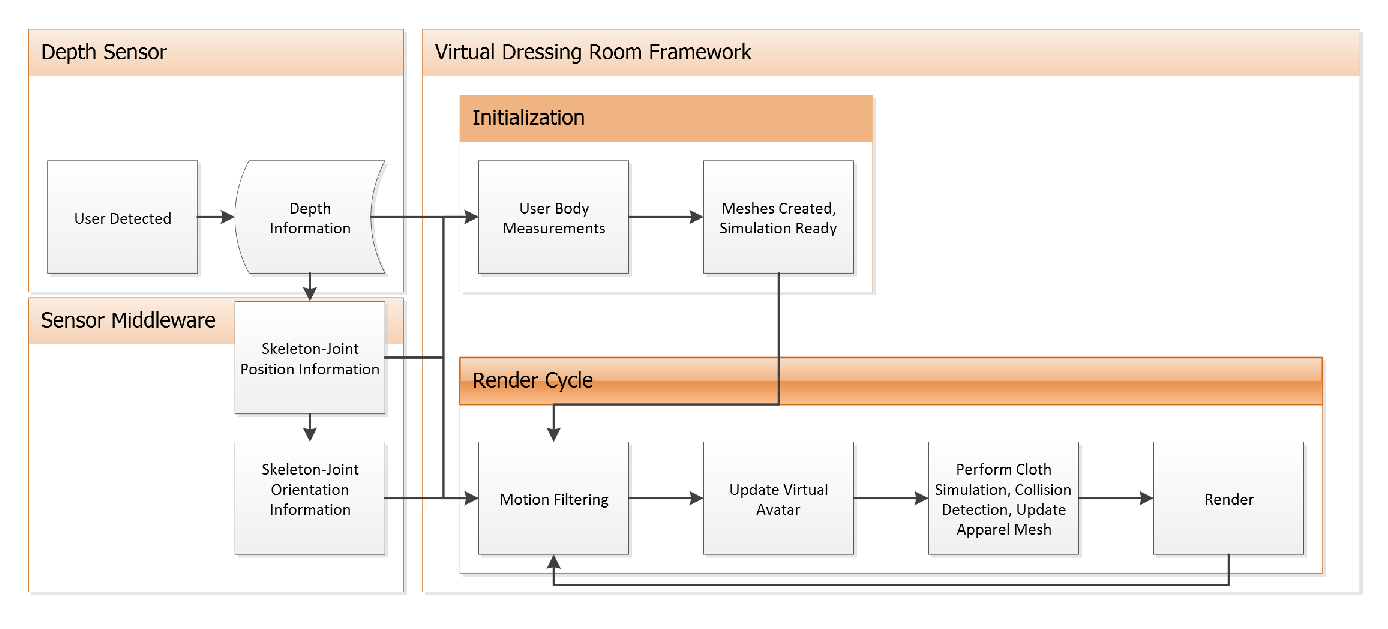
\includegraphics[width=1.0\textwidth]{./figures/overall.eps}
	}
	\caption{The overall virtual dressing framework}
	\label{fig:overall}
\end{figure}

\subsection{Physics Engine}
\label{subsec:Physics}
The cloth simulation framework utilizes the proprietary PhysX engine by Nvidia~\cite{Kim2011}, with two major components as the {\em cloth deformation} and {\em collision detection} modules. 

The deformation algorithm is based on the position-based dynamics approach~\cite{Mullera2007}, calculating the position of the particles from their previous positions and applying constraints on mutual distance and angle. The approach is stable and efficient for real time applications. 

Collision between the body and the cloth is detected using collision spheres and capsules (composed of two spheres) co-located with body joints and bones, respectively (cf.~Figure~\ref{fig:colliders}). The female body bone information is extracted from the input skeletal mesh and the colliding capsules are generated automatically after the measurement process, with the capsule pair indexes stored in an array.

\begin{figure}[htbp]
	\begin{center}
	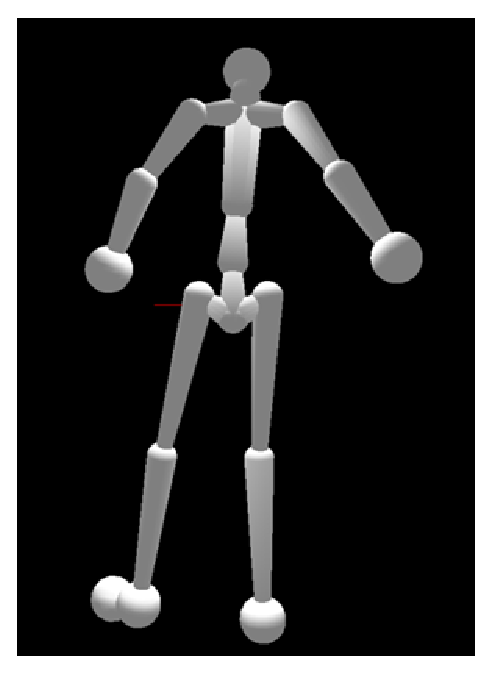
\includegraphics[width=0.70\textwidth]{./figures/colliders.eps}
	\end{center}
	\caption{The colliding human body with the default radii}
	\label{fig:colliders}
\end{figure}

The solution is performed for the trajectory of the capsule or sphere and the particle for each frame interval. This approach is especially robust in fast motion, which is important because the motion is created in real time. The resulting equation is a sixth degree polynomial, which is approximated with a quadratic equation. The solution is performed on the GPU, which increases the parallel performance greatly, allowing for frame rates higher than 600 frames per second (fps). The cloth is discretized as a triangle mesh and the collision is only detected on vertices, therefore density must be high enough in order to avoid penetration at locations further from the vertices~\cite{Kim2011,Tonge2010}. This issue can be resolved using virtual particles for apparel meshes with lower resolution, where additional vertices are introduced at runtime for collision simulation~\cite{Kim2011}.

The acquired body measurements are used to estimate the locations of joints and bones, for collision sphere placement, whereas the radii are used directly for determining the sphere sizes. With both parameters scaled according to the user, various body types can be simulated realistically.

\subsection{Body Measurements}
\label{subsec:Measurements}
For a realistic fitting experience, another requirement is acquiring a set of simulation parameters from a human test-subject for a pre-modeled apparel mesh, which is to be displayed on a virtual avatar reflecting the body characteristics of the aforementioned subject.  The set of parameters for the simulation includes the body height and width, also the radii for the collision spheres, which have their centers coinciding with the joints of the virtual avatar's skeleton.
The body width and height are then utilized to estimate the body size of the user, collision spheres are used in the dressing room simulation, to detect and resolve collision with the cloth particles.

As opposed to the studies focusing on acquiring high-detail avatars of subjects for made-to measure applications, we focus on the speed of the overall algorithm for real-time purposes and acquire enough measurements for a 'fixed-size try-on' system.   
  
\subsubsection{Depth Map Filtering}
\label{subsubsec:4.1} 
The state-of the art time-of-flight (TOF) cameras still provide low resolution and quality output compared to the state-of-the-art advanced RGB systems. The quality of the input depth map is a crucial factor on the overall performance of the system, therefore, we first wish to improve the quality of the depth map by applying canonical image enhancement methods.

In this approach, we utilize a TOF camera running with a middleware that provides a subject map. The subject map has the same size as the depth map. It has the same origin as the pixels of the depth map, either belonging to a subject or to the background.

Let us take the input depth map $D$ as a $M \times N$ matrix. Initially, the user pixels from $D$ are extracted by a pixel-by-pixel comparison with the input user map. We are only interested in the one subject and $D_1$ represents the depth pixels of him, whereas $U_1$ is the bit map of the subject. Also, the non-subject pixels are set to the mean value of the user pixels, to set the matrix properly for the subsequent filterings.

\begin{equation}
D_1=(D-(D \times U_1 )) \times \frac{1}{n} \times \sum\limits_{i=0}^n \left(\left(D \times U_1 \right)_i + d \times U_1 \right)
\label{eqn:patch_depth}
\end{equation}

The subject depth map is now prepared to be processed with Gaussian filtering to normalize and improve the quality. 

\begin{equation}
D_G\;=\;D_1\;*\;G, 
\label{eqn:gaussian_convolution}
\end{equation}

\noindent where `$*$' is the convolution operator. The Gaussian filtering completes the enhancement of the input depth map. 
The overall process is described in Algorithm \ref{algo:depth_patch}.

\singlespacing

\begin{algorithm}
\DontPrintSemicolon 
\KwIn{Raw depth and subject stream from the depth sensor}
\KwOut{Optimized subject map}
$depth_{\textit{sum}}=0$ \;
$n_{\textit{user}} =0$\;
\For{i \bf{from} 0 \bf{to} $d_{\textit{width}}$ }{
\For{j \bf{from} 0 \bf{to} $d_{\textit{height}}$ }{
\If{$U(i,j)$} {
  $depth_{\textit{sum}}=depth_{\textit{sum}}+D(i,j)$\;
  $n_{\textit{user}}+=1$\;
 }}}
$depth_{\textit{average}}=depth_{\textit{sum}}/n_{\textit{user}}$ \;
\For{i \bf{from} 0 \bf{to} $d_{\textit{width}}$ }{
\For{j \bf{from} 0 \bf{to} $d_{\textit{height}}$ }{
\If{\bf{not}  $U(i,j)$} {
  $D(i,j)=depth_{\textit{average}}$\;
 }}}
 
\For{i \bf{from} 0 \bf{to} $d_{\textit{width}}$ }{
\For{j \bf{from} 0 \bf{to} $d_{\textit{height}}$ }{
\If{$U(i,j)$} {
  \tcp{`*' denotes convolution operator}
  $D(i,j)=D(i-m:i+m, j-n:j+m) * Gaussian(m,n,e)$\; 
 }}}
 
\Return{D}
\caption{Depth Map Filtering}
\label{algo:depth_patch}
\end{algorithm}

\doublespacing

\subsubsection{Body Measurement}
\label{subsubsec:4.2} 

By now, we have an optimized depth map, which is ready for performing key body dimension measurements. The key dimensions are handled in two groups: the collision sphere radii, which are used for the collision detection in the simulation, and the height and width parameters, which are used to determine to size of the apparel. 

\paragraph{Collision Sphere Radii:}

The simulation framework utilizes collision spheres and capsules instead of arbitrary geometries. This constraint allows the simulation to run in real time with exceptionally high frame rates by simplifying the algorithms. There are a total of 15 joint locations provided by the middleware, as shown in Figure~\ref{fig:nite_joints}. These are the key points for collision sphere placement. For this reason, the framework also utilizes 15 collision spheres and the capsules formed by pairs.

\begin{figure}[htbp]
	\begin{center}
	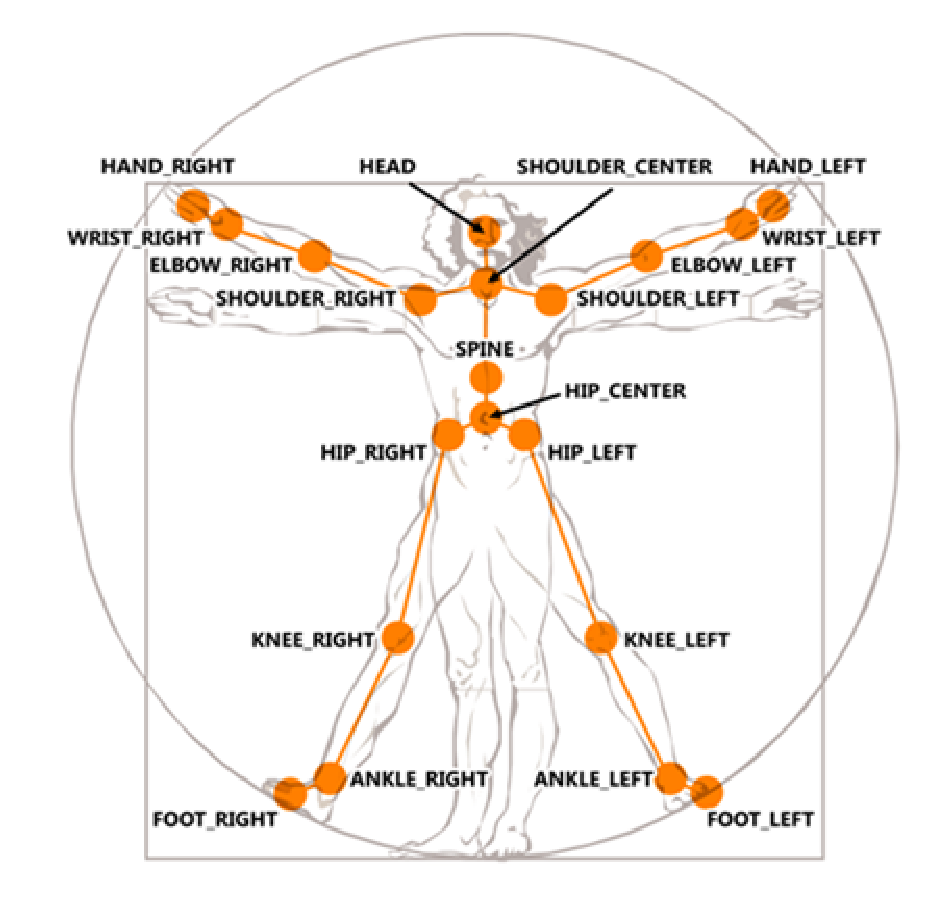
\includegraphics[width=0.85\textwidth]{./figures/nite_joints.eps}
	\end{center}
	\caption{Human joints provided by Kinect SDK~\cite{CodeProject2011}.}
	\label{fig:nite_joints}
\end{figure}

For a realistic simulation, collision spheres must be as large as possible without intersecting the skin mesh of the avatar. The optimal sphere fitting algorithm starts with an infinitely small circle and expands it discretely until it intersects with the body contour. The steps of this algorithm are as follows:  

\begin{enumerate}
\item Take vector $J_i$, which represents the coordinates of the $i^{th}$ joint.
Initialize the radius of the sphere by setting it to the z-distance with the overlapping point in the depth map.
\begin{equation}
r_i^z=J_i^z-D^z(J_i^x,J_i^y)
\label{eqn:z_sphere_radius}
\end{equation}
\item Start with an infinitely small line segment parallel to the x-axis. Expand it until it intersects with the body contour. Take the x-distance between the intersection point and the joint location. Repeat the same process with a line segment parallel to the y-axis and take the larger radius. While expanding the segment, stop expanding and discard the corresponding result if the border of the depth map is reached.
\begin{equation}
r_i^{x,y}=max(|J_i^{x,y} \; - \; D^{x,y}(J_i^{y,x},J_i^z)|)
\label{eqn:x_y_sphere_radius}
\end{equation}
\item Take the minimum of the radii of the three axes because there should be no intersection with the body contour and the shape must be a sphere.
\begin{equation}
r_i=min(r_i^{x, y, z})
\label{eqn:minimum_sphere-radius}
\end{equation}
\end{enumerate}

\noindent The pseudocode of the optimal sphere fitting is given in Algorithm~\ref{algo:sphere_fitting}.

\singlespacing

\begin{algorithm}
\DontPrintSemicolon 
\KwIn{Optimized depth stream from the depth sensor}
\KwOut{Collision sphere radii for each joint}
\ForEach{joint}{
$p=pos_{J_m}$\;
$r_z=\sqrt{P_z^2-D_z(P_x,P_y)^2}$\;
\For{i \bf{from} $P_x$ \bf{to} $0$ }{
\If{$D(i,P_y)$ \bf{equals}  $P_z$} {
  $r_{x^{-}} = i$\;
  break\;
 }
}
\For{i \bf{from} $P_x$ \bf{to} $\textit{depth}_{\textit{width}}$ }{
\If{$D(i,P_y)$ \bf{equals}  $P_z$} {
  $r_{x^{+}} = i$\;
  break\;
 }
}
\For{j \bf{from} $P_y$ \bf{to} $0$ }{
\If{$D(P_x,j)$ \bf{equals}  $P_z$} {
  $r_{y^{-}} = j$\;
  break\;
 }
}
\For{j \bf{from} $P_y$ \bf{to} $\textit{depth}_{\textit{height}}$ }{
\If{$D(P_x,j)$ \bf{equals}  $P_z$} {
  $r_{y^{+}} = j$\;
  break\;
 }
}
$r_m=min(r_z,\; r_{x^{-}}, \; r_{x^{+}},\; r_{y^{-}}, \; r_{y^{+}})$
}
\Return $(r_{0}, \; r_{1} \; \ldots \; r_{n})$ 
\caption{Sphere Fitting Algorithm}
\label{algo:sphere_fitting}
\end{algorithm}  

\doublespacing

\paragraph{Height and Width Parameters:}

The width and height of the subject is important for determining the proper actual size for the cloth. However, a straightforward 
estimation of the body height and shoulder width is prone to errors due to the noise and quality of the incoming depth map. In 
order to minimize this error, an upscaled version of the subject's body is measured, to be used in width-height estimation 
later. We use the human body proportions defined by~\cite{Willis2012}, which are shown in Table~\ref{tbl:human_body_proportions}. 
For the sake of relative representation, the width and height of the head are taken as unit width and height, respectively. The 
measurement source column in the table represents the source for the estimation of the respective parameter:
\begin{itemize} 
\item
The joint location represents that the measurement will take the input subject joint locations as the reference.
\item 
The depth map represents the measurement will instead perform measurements based on the pixel distribution in the filtered subject depth map. 
\end{itemize}
They are often used together for better performance. Please note that some of these parameters are not standard to be used as relative references, such as the hip width. These parameters do not effect others in the estimation process and vice versa.

\begin{figure}
	\begin{center}
			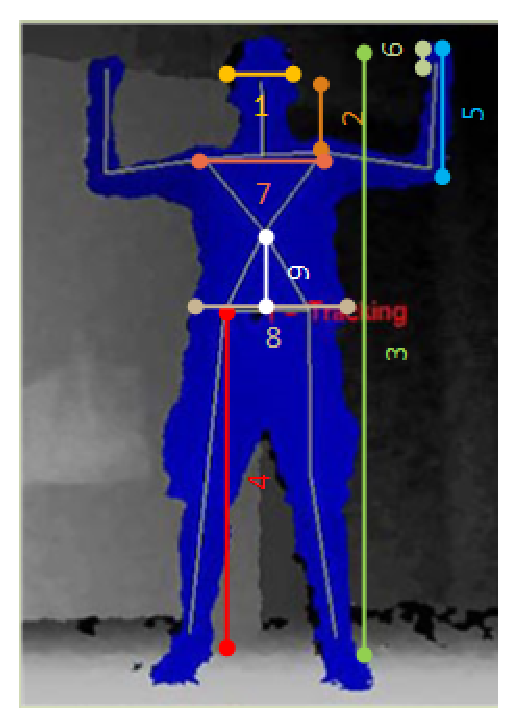
\includegraphics[width=0.70\columnwidth]{./figures/body_proportions.eps}
	\end{center}
	\caption{Human body proportions.}
	\label{fig:body_proportions}
\end{figure}

\singlespacing
\begin{table}
\begin{center}
\begin{tabular}{|l|c|c|l|}
\hline
\textbf{Distance} & \textbf{Width} & \textbf{Height} & \textbf{Measurement} \\ 
\textbf{        } & \textbf{     } & \textbf{      } & \textbf{Source} \\ \hline
Head & 1w (1) & 1h (2) & Depth Map + \\ 
     &        &        & Joint Location \\ \hline
Body Height & - & 7h (3) & Depth Map \\ \hline
Hip Height & - & 4h (4) & Joint Location \\ \hline
Elbow to & - & 2h (5) & Depth Map + \\ 
Fingertip &   &       & Joint Location \\ \hline
Wrist to  & - & 1h (6) & Depth Map + \\ 
Fingertip &   &       & Joint Location \\ \hline
Shoulder  & 3w (7) & - & Depth Map + \\ 
Width     &  &   & Joint Location \\ \hline
Hip Width & - (8) & - & Depth Map \\ \hline
Torso Height & - & - (9) & Joint Location \\ 
\hline
\end{tabular}
\end{center}
\caption{Human body proportions. The numbers in parentheses correspond 
to the lines in Figure~\ref{fig:body_proportions}.}
\label{tbl:human_body_proportions}
\end{table}

\doublespacing

The measurements are performed in the real-world space, rather than the projective space, because a real size estimation is crucial for determining the appropriate cloth size. The latter would be sufficient for simulation purposes, when there is no concern of real-life apparel fitting. After the acquisition of the required scaling parameters for the subject, the cloth and avatar should be scaled as a whole in three dimensions uniformly, in contrast to a segmented scaling. This decision is based on the scope of our work because it is a standard-sized apparel fitting application without extensive customization. Following the measurements, the body width and shoulder height are estimated as follows:

\clearpage

\begin{enumerate}
\item Take the primary dimension (either the body height or shoulder width) $P_i^0$. This process is repeated for width (W) and height (H).
\item Using the remaining measurements in the set, estimate the primary dimension $P_i$ as $P_i^j$ using proportion $R_i^j$ from \ref{tbl:human_body_proportions}.
\begin{equation}
W,H_i^j=W,H_j \times R_i^j
\label{eqn:proportion_estimation}
\end{equation}
\item Find the optimized primary dimension as the mean of all estimations:
\begin{equation}
W,H_i=\frac{1}{(n+1)} \times \sum\limits_{j=0}^n W,H_i^j
\label{eqn:optimized_parameter}
\end{equation}
\end{enumerate}

\singlespacing

\begin{algorithm}
\DontPrintSemicolon 
\KwIn{Human body proportions and the user and depth data}
\KwOut{The body width and shoulder height}
$t_{\textit{proportion}}=import(\mbox{Table}~\ref{tbl:human_body_proportions})$ \;
$t_{\textit{primary}}= (w_{\textit{shoulder}}, \; h_{\textit{body}})$ \;
$ct={\textit{cloth}}_{\textit{type}}$\;
${\textit{width}}_{\textit{main}}=t_{\textit{proportion}}.width(ct)$\;
${\textit{width}}_{\textit{sum}}=0$\;
${\textit{count}}_{\textit{effector}}=0$\;
\ForEach{{\textit{width}} \bf{in} $t_{\textit{proportion}}$ }{
$w_i=\textit{measure}(p_i)$\;
$w_i^j=w \times t_{\textit{proportion}}.\textit{ratio}(p_i,\textit{\textit{width}}_{\textit{main}})$\;
${\textit{width}}_{\textit{sum}}={\textit{width}}_{\textit{sum}}+w_i^j $\;
${\textit{count}}_{\textit{effector}}++ $\;
}
${\textit{width}}_{\textit{weighted}}=\frac{\textit{\textit{width}}_{\textit{sum}}}{\textit{count}_{\textit{effector}}}$\;
$x_s=\frac{\textit{\textit{width}}_{\textit{weighted}}}{\textit{\textit{width}}_{\textit{cloth}}}$\;

${\textit{height}}_{\textit{main}}=t_{\textit{proportion}}.{\textit{height}}(ct)$\;
${\textit{height}}_{\textit{sum}}=0$\;
$\textit{count}_{\textit{effector}}=0$\;
\ForEach{{\textit{height}} \bf{in} $t_{\textit{proportion}}$ }{
$h_i={\textit{measure}}(p_i)$\;
$h_i^j=h \times t_{\textit{proportion}}.\textit{ratio}(p_i,\textit{\textit{height}}_{\textit{main}})$\;
${\textit{height}}_{\textit{sum}}={\textit{height}}_{\textit{sum}}+h_i^j $\;
${\textit{count}}_{\textit{effector}}++ $\;
}
$\textit{\textit{height}}_{\textit{weighted}} = \frac{\textit{\textit{height}}_{\textit{sum}}}{\textit{count}_{\textit{effector}}}$\;
$y_{s}=\frac{\textit{\textit{height}}_{\textit{weighted}}}{\textit{\textit{height}}_{\textit{cloth}}}$\;
\Return{$(x_s, \; y_s)$}
\caption{Body Dimension Estimation}
\label{algo:cloth_resize}
\end{algorithm}

\doublespacing

\subsubsection{Temporal Optimization}
\label{subsec:4.3} 

By now, we have acquired the required body dimensions and collision sphere parameters for a realistic simulation. 
Yet, the measurements are performed on a filtered version of a depth sensor with high error rates. In order to overcome the noise and overall depth-sense faults, the prior measurements are repeated for the duration of one second, which corresponds to 30 frames of input depth map. 
A considerably different approach here would be to employ the temporal averaging on the depth map instead of the measured parameters. We observe that the results suffer due to the motions of the subject because most subjects fails to keep their exact form for one second. To overcome these problems, we use temporal averaging that takes the mean of the specified parameters for the frames in one second. This step finalizes the parameters and delivers the required parameters for simulation environment synthesis. 

\singlespacing

\begin{algorithm}
\DontPrintSemicolon % Some LaTeX compilers require you to use \dontprintsemicolon instead
\KwIn{Raw depth stream from the depth sensor}
\KwOut{Final collision sphere radii and body dimensions}
\tcp{s is a buffer for storing x and y scaling parameters for 30 frames}
\tcp{r is a buffer for storing for collision sphere radii of 16 joints for 30 frames}
float s[30, 2], r[30, 16] \;
\For{i \bf{from} 0 \bf{to} $30 frames$ }{
	r[i][1:16]=fitSpheres()\;
	s[i][1:2]=optimizeScaleParameters()\;
}
$r_{\textit{final}}$  = \textrm{avg}(r)\;
$s_{\textit{final}}$  = \textrm{avg}(s)\;
\caption{Temporal Averaging}
\label{algo:temporal_averaging}
\end{algorithm}

\doublespacing


\subsection{Motion Smoothing}
\label{subsec:Motion}
Our framework utilizes a virtual 3D avatar to display and simulate the apparel models. The avatar imitates the motions of the actual user, using the orientation data acquired from the depth sensor middleware. However, application of the raw data from the sensor causes unnatural movements due to the noise in the sensor input, self-occlusions of the body and inadequate IK solvers.  In order to present a more realistic avatar animation, a series of filters and constraints are applied to the sensor data. 

\subsubsection{Position Filtering}
The most severe disruption of the self-occlusion problem takes place in the joint position acquisition. There is no possible way of acquiring the correct position of a limb when the sensor has no vision of it. However, the way humans move their limbs under normal conditions follow certain principles and trends, which can be used to estimate the locations of occluded body parts. The nature of these motions, demonstrating traits similar to seasonal behavior, makes them suitable for applying a variety of filters~\cite{Azimi2012}. We decided to go with the Holt-Winters double exponential smoothing~\cite{Holt1957,Kalekar2004} as it comes with the middleware, easy to use and delivers good quality results with acceptable latency for the purposes of this application. 

\subsubsection{Rotation Filtering and Constraints}
The joint orientations are acquired from the sensor middleware directly, however the data is not smooth. Although the middleware enforces certain constraints (such as allowing only pitch rotations on ulna), there are often significant gaps in the estimated angles that produce unnatural tremor-like movements on the avatar. Furthermore, there is no filtering of unnatural rotations that take place when an occluded body part is estimated to be in a wrong location. 

The inferior quality of the orientation data is improved in two stages: applying another set of constraints on the joint data based on the natural limits of human bones, followed by an asymptotic smoothing of the joint angles to prevent the effect of gaps in the angles (see~Figure~\ref{fig:rotation-filter}). 

\begin{figure}[htbp]
	\centerline{
	\fbox{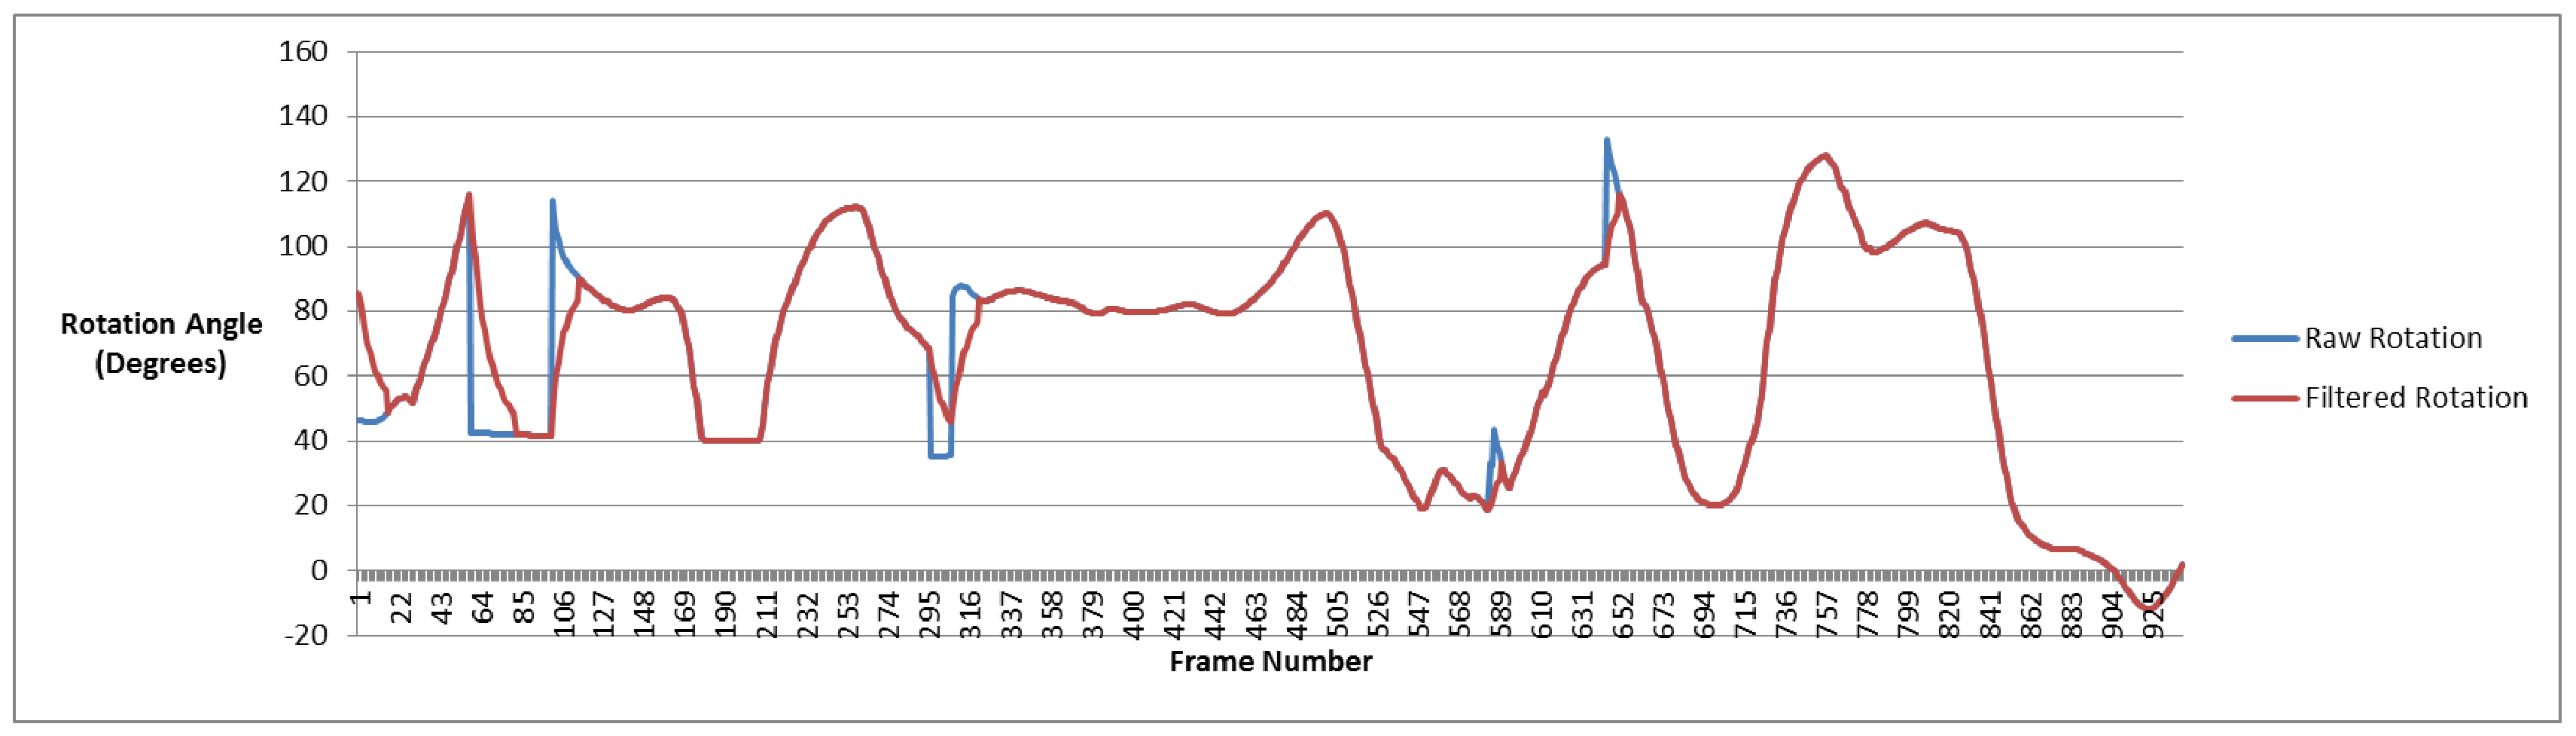
\includegraphics[width=0.98\textwidth]{./figures/rotation-filter.eps}}
	}
\centerline{\ }
\caption{The row and filtered samples for right the humerus roll angle}
	\label{fig:rotation-filter}
\end{figure}


\subsubsection{Bone Splitting}
The lower sections of human limbs contain two parallel bones allowing the twisting rotation on the hands and feet. The configurations of bones allow all portions of the lower limbs follow the bones in pitch and roll rotations, although the effect of yaw rotation decreases as it gets closer to the mid-section joint (elbow or knee). This effect is not possible to achieve with a single bone fore-arm representation, as specified in the highest level of detail in the H-ANIM standard~\cite{HANIM}, using unified weights (same for all types of rotations, transformations and scaling) and linear skinning. On the other hand, applying a different set of weights for each possible transformation, rotation or scaling requires additional space and time, which can be considered redundant because it is not going to be used in most parts of the skeleton and surface mesh; thus, it is not implemented in most of the popular rendering engines. This problem is addressed by Kavan et al.~\cite{Kavan2009}, proposing a method of introducing additional blending bones to simulate non-linear skinning. However, this approach is not suitable for a real-time application with previously unknown motions. 

Because our only problematic bones for this particular case is the upper limbs, we employed a novel approach to solve this problem by introducing an additional bone connected in series for the upper limbs. The humerus and ulna bones are split halfway and the lower sections are labeled as humerus-extension and ulna-extension, respectively. The vertex weights in the corresponding sections are divided linearly among two sections, as seen in Figure~\ref{fig:forearm-weights}. 


\begin{figure}[htbp]
	\centerline{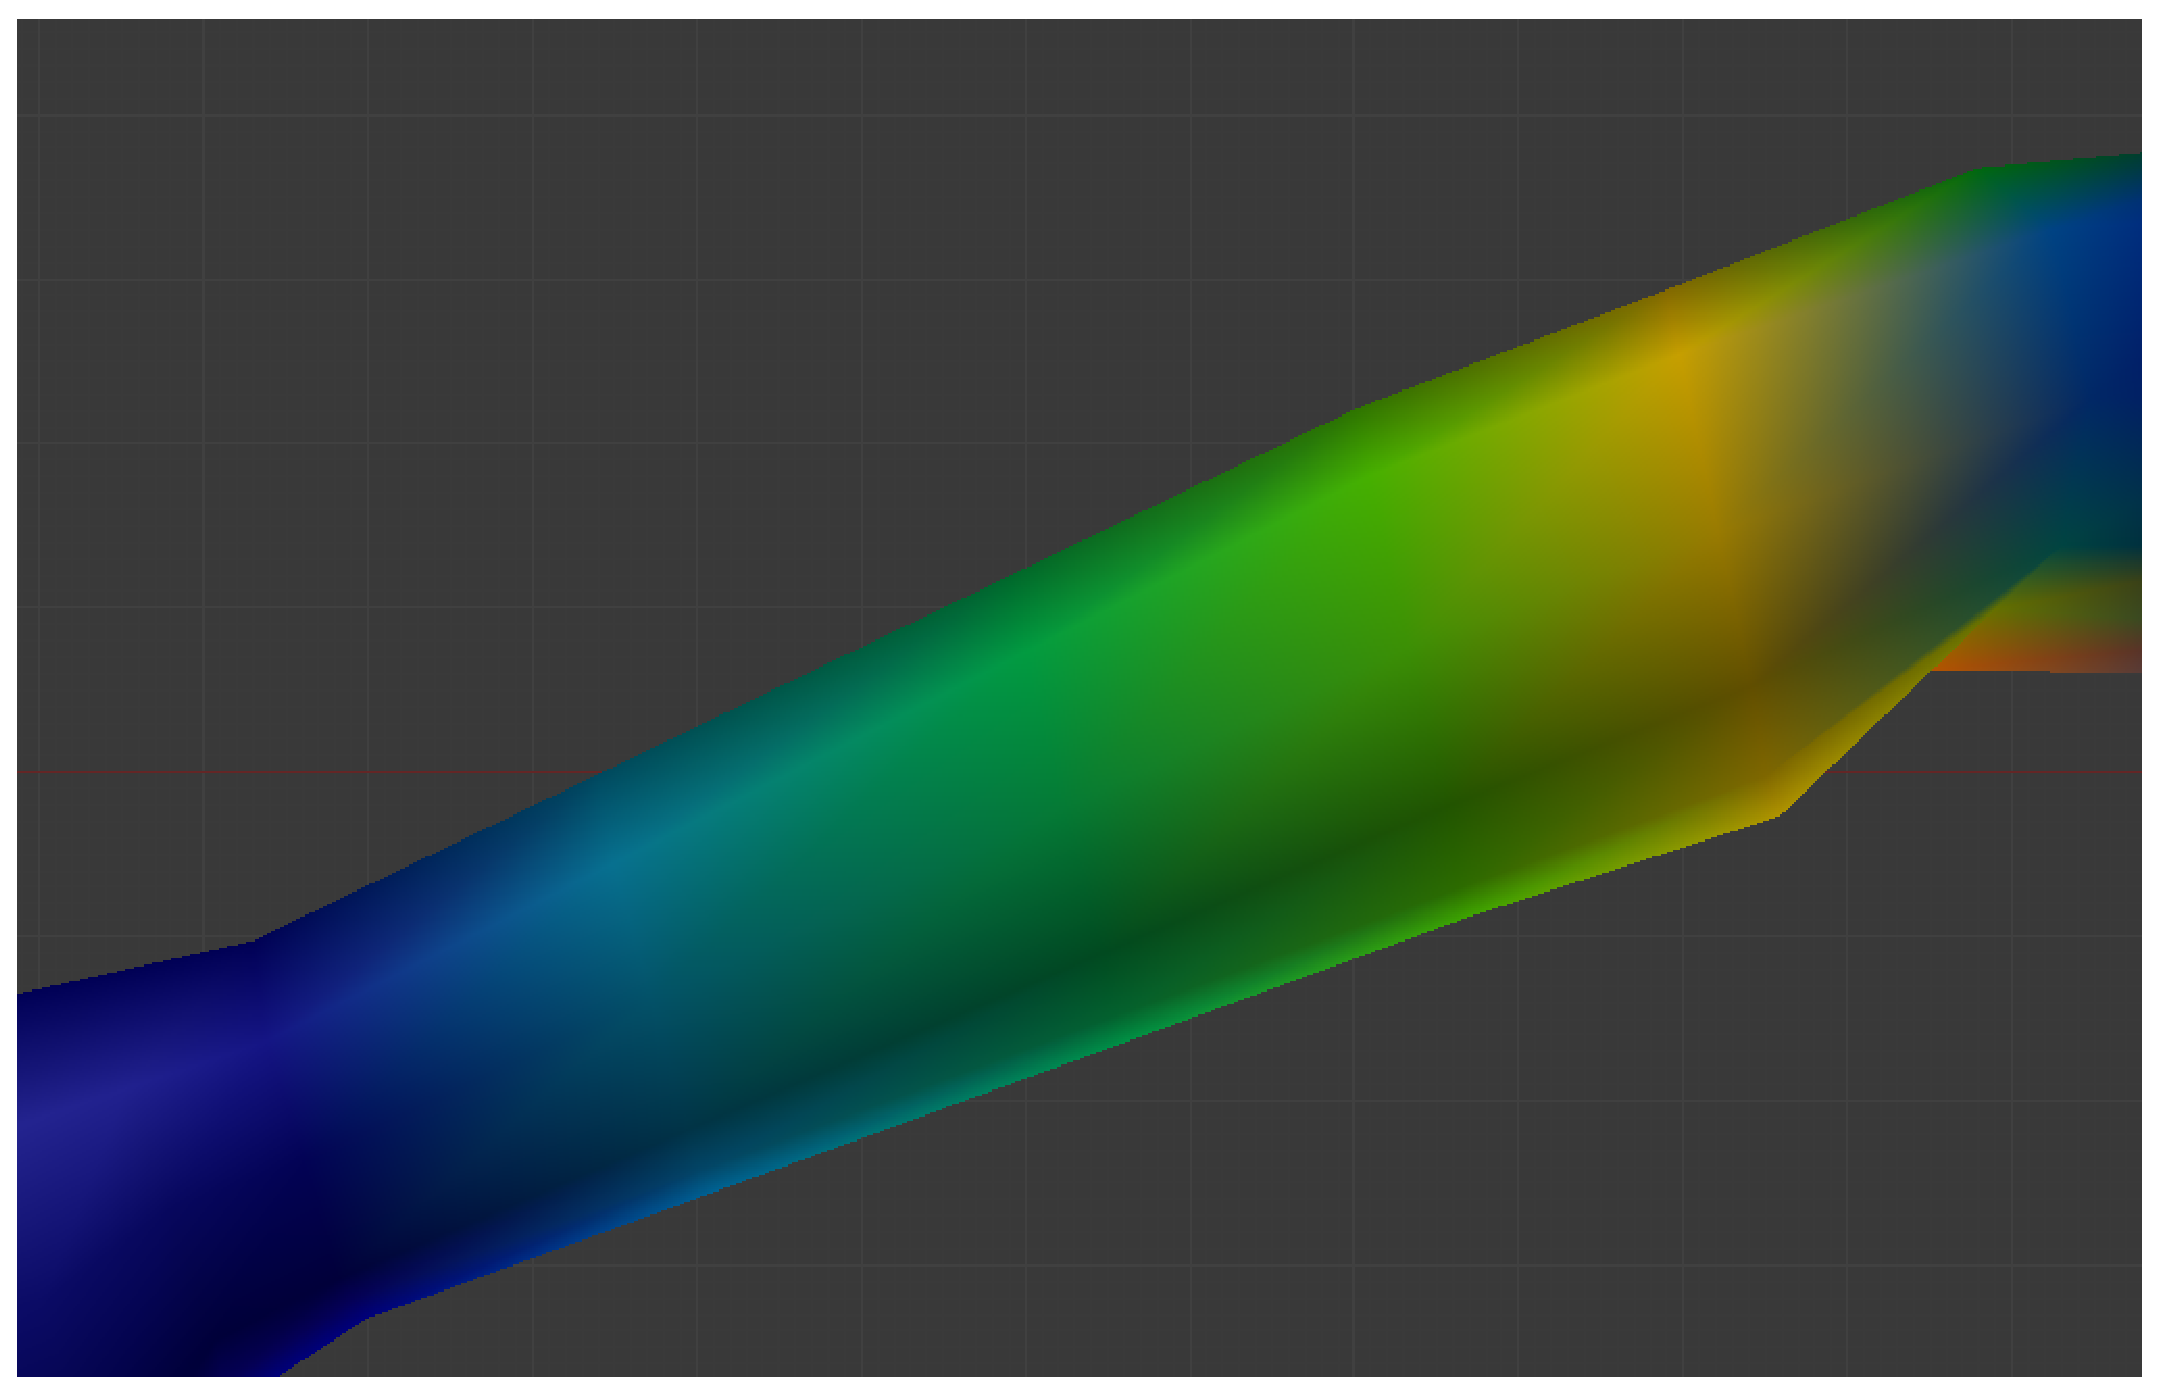
\includegraphics[width=0.75\textwidth]{./figures/ulna-weight.eps}}
	\centerline{(a)}
	\centerline{\ }
	\centerline{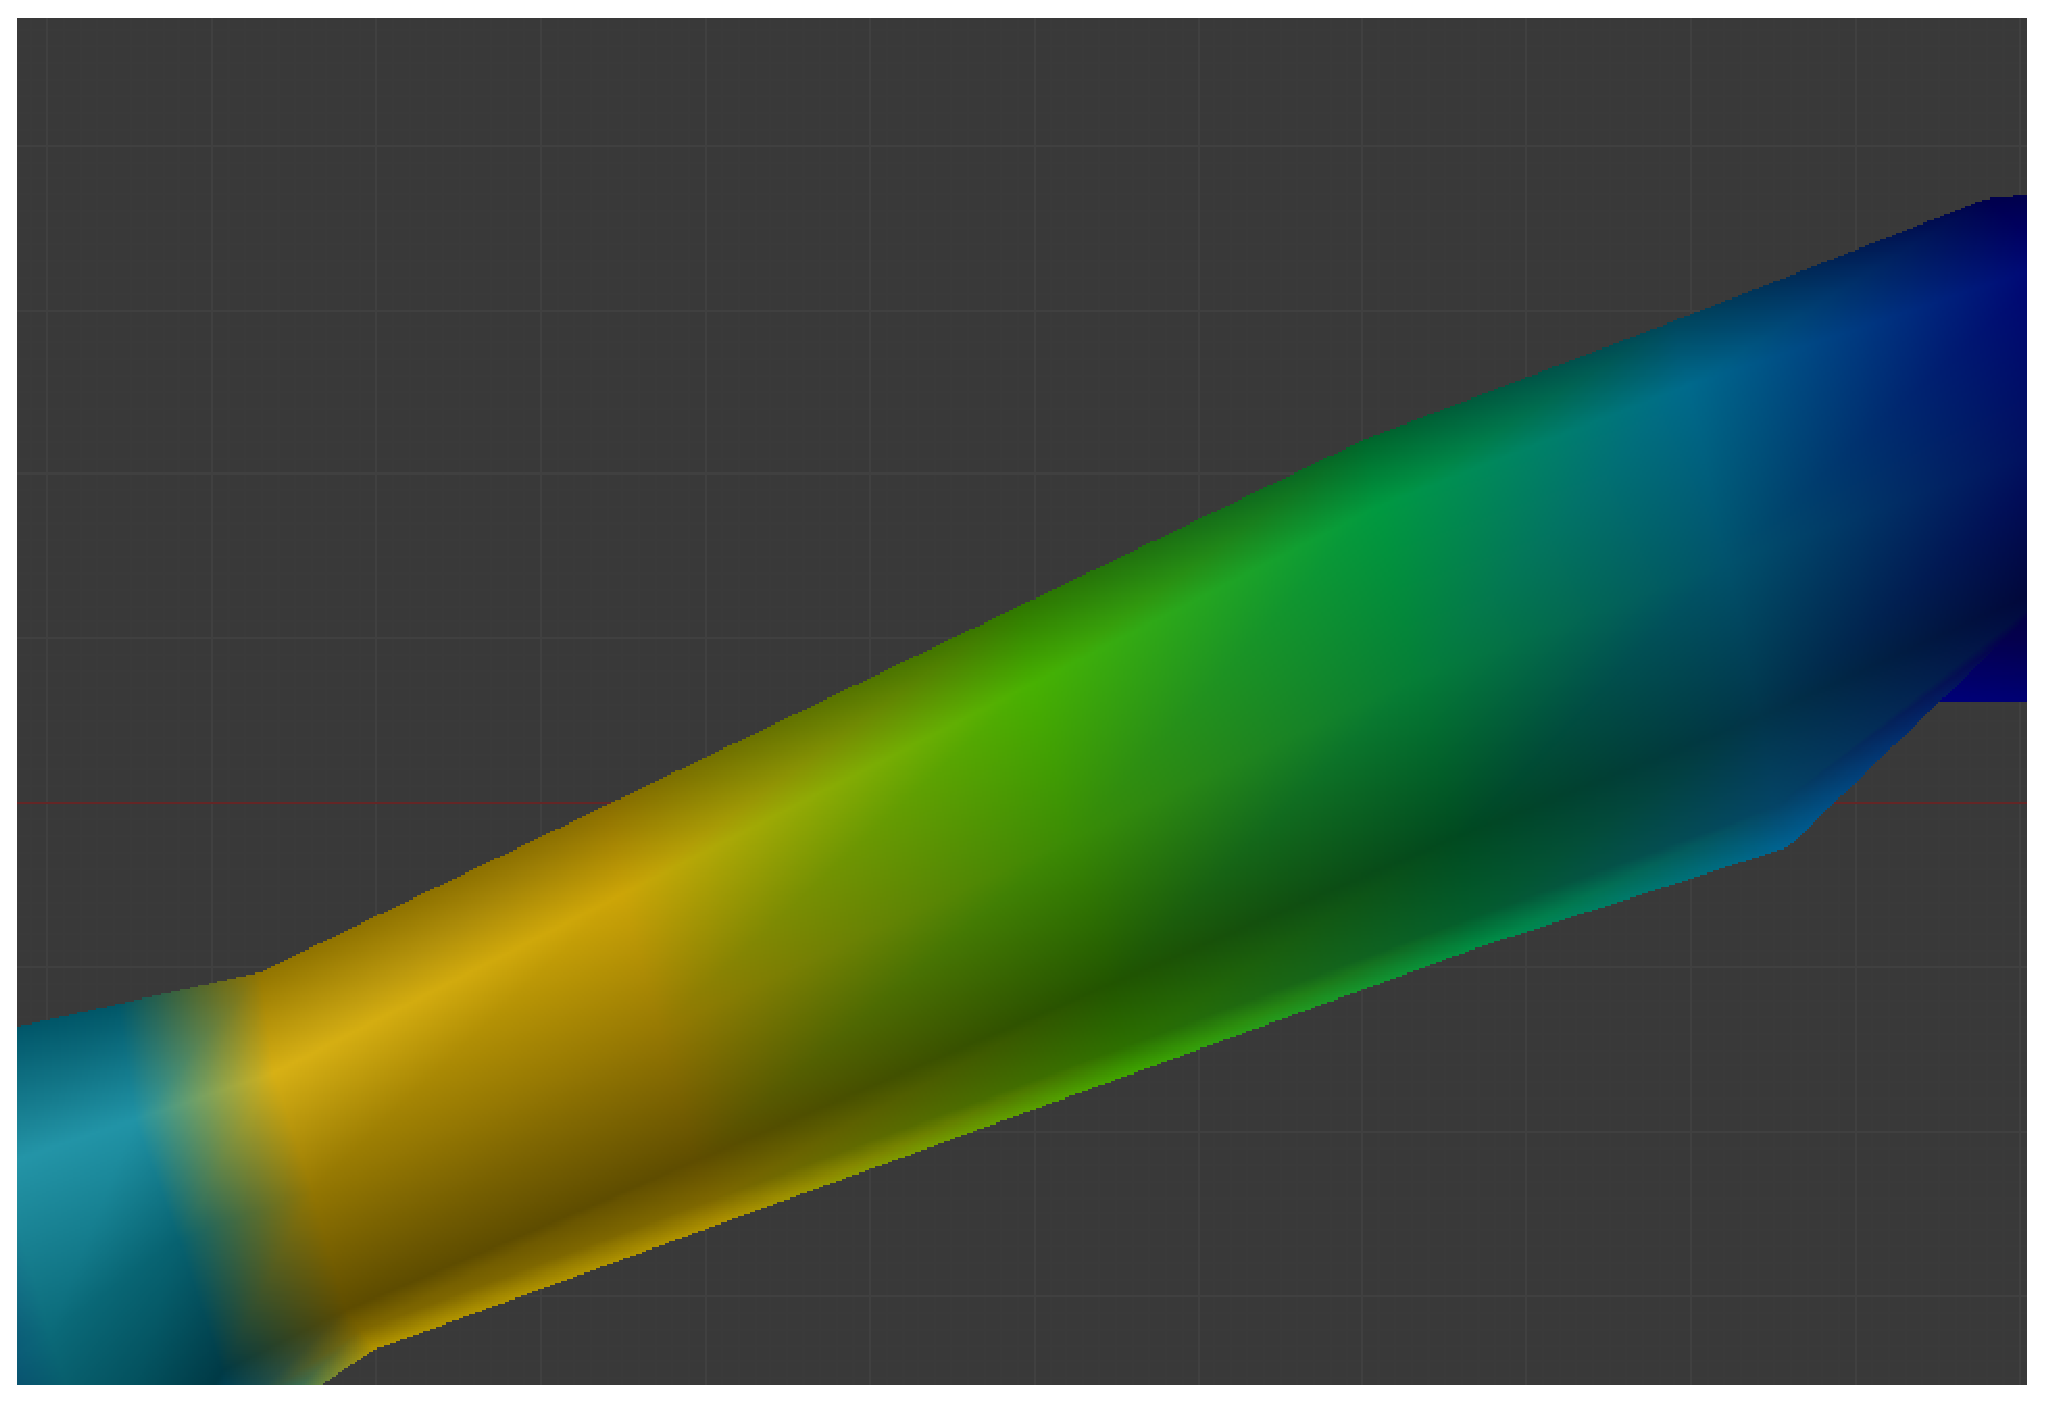
\includegraphics[width=0.75\textwidth]{./figures/ulna-extent-weight.eps}}
	\centerline{(b)} 
	\centerline{\ } 
	\caption{The vertex weights for (a) the upper ulna and (b) the lower ulna bone (weight increases from blue to yellow).}
	\label{fig:forearm-weights}
\end{figure}

During runtime, the filtered local rotation of the upper limb bones are separated into two distinct rotations, one containing the yaw and the other containing pitch and roll rotations, which are applied to the extension bone and the original bone, respectively. With proper weights, the rotation of the users arm is transferred to the virtual avatar naturally without introducing any artifacts. As seen in Figure~\ref{fig:forearm-comparison}, the vertices on the forearm twist in a more natural way resembling the real motion.

\begin{figure}[htbp]
	\centerline{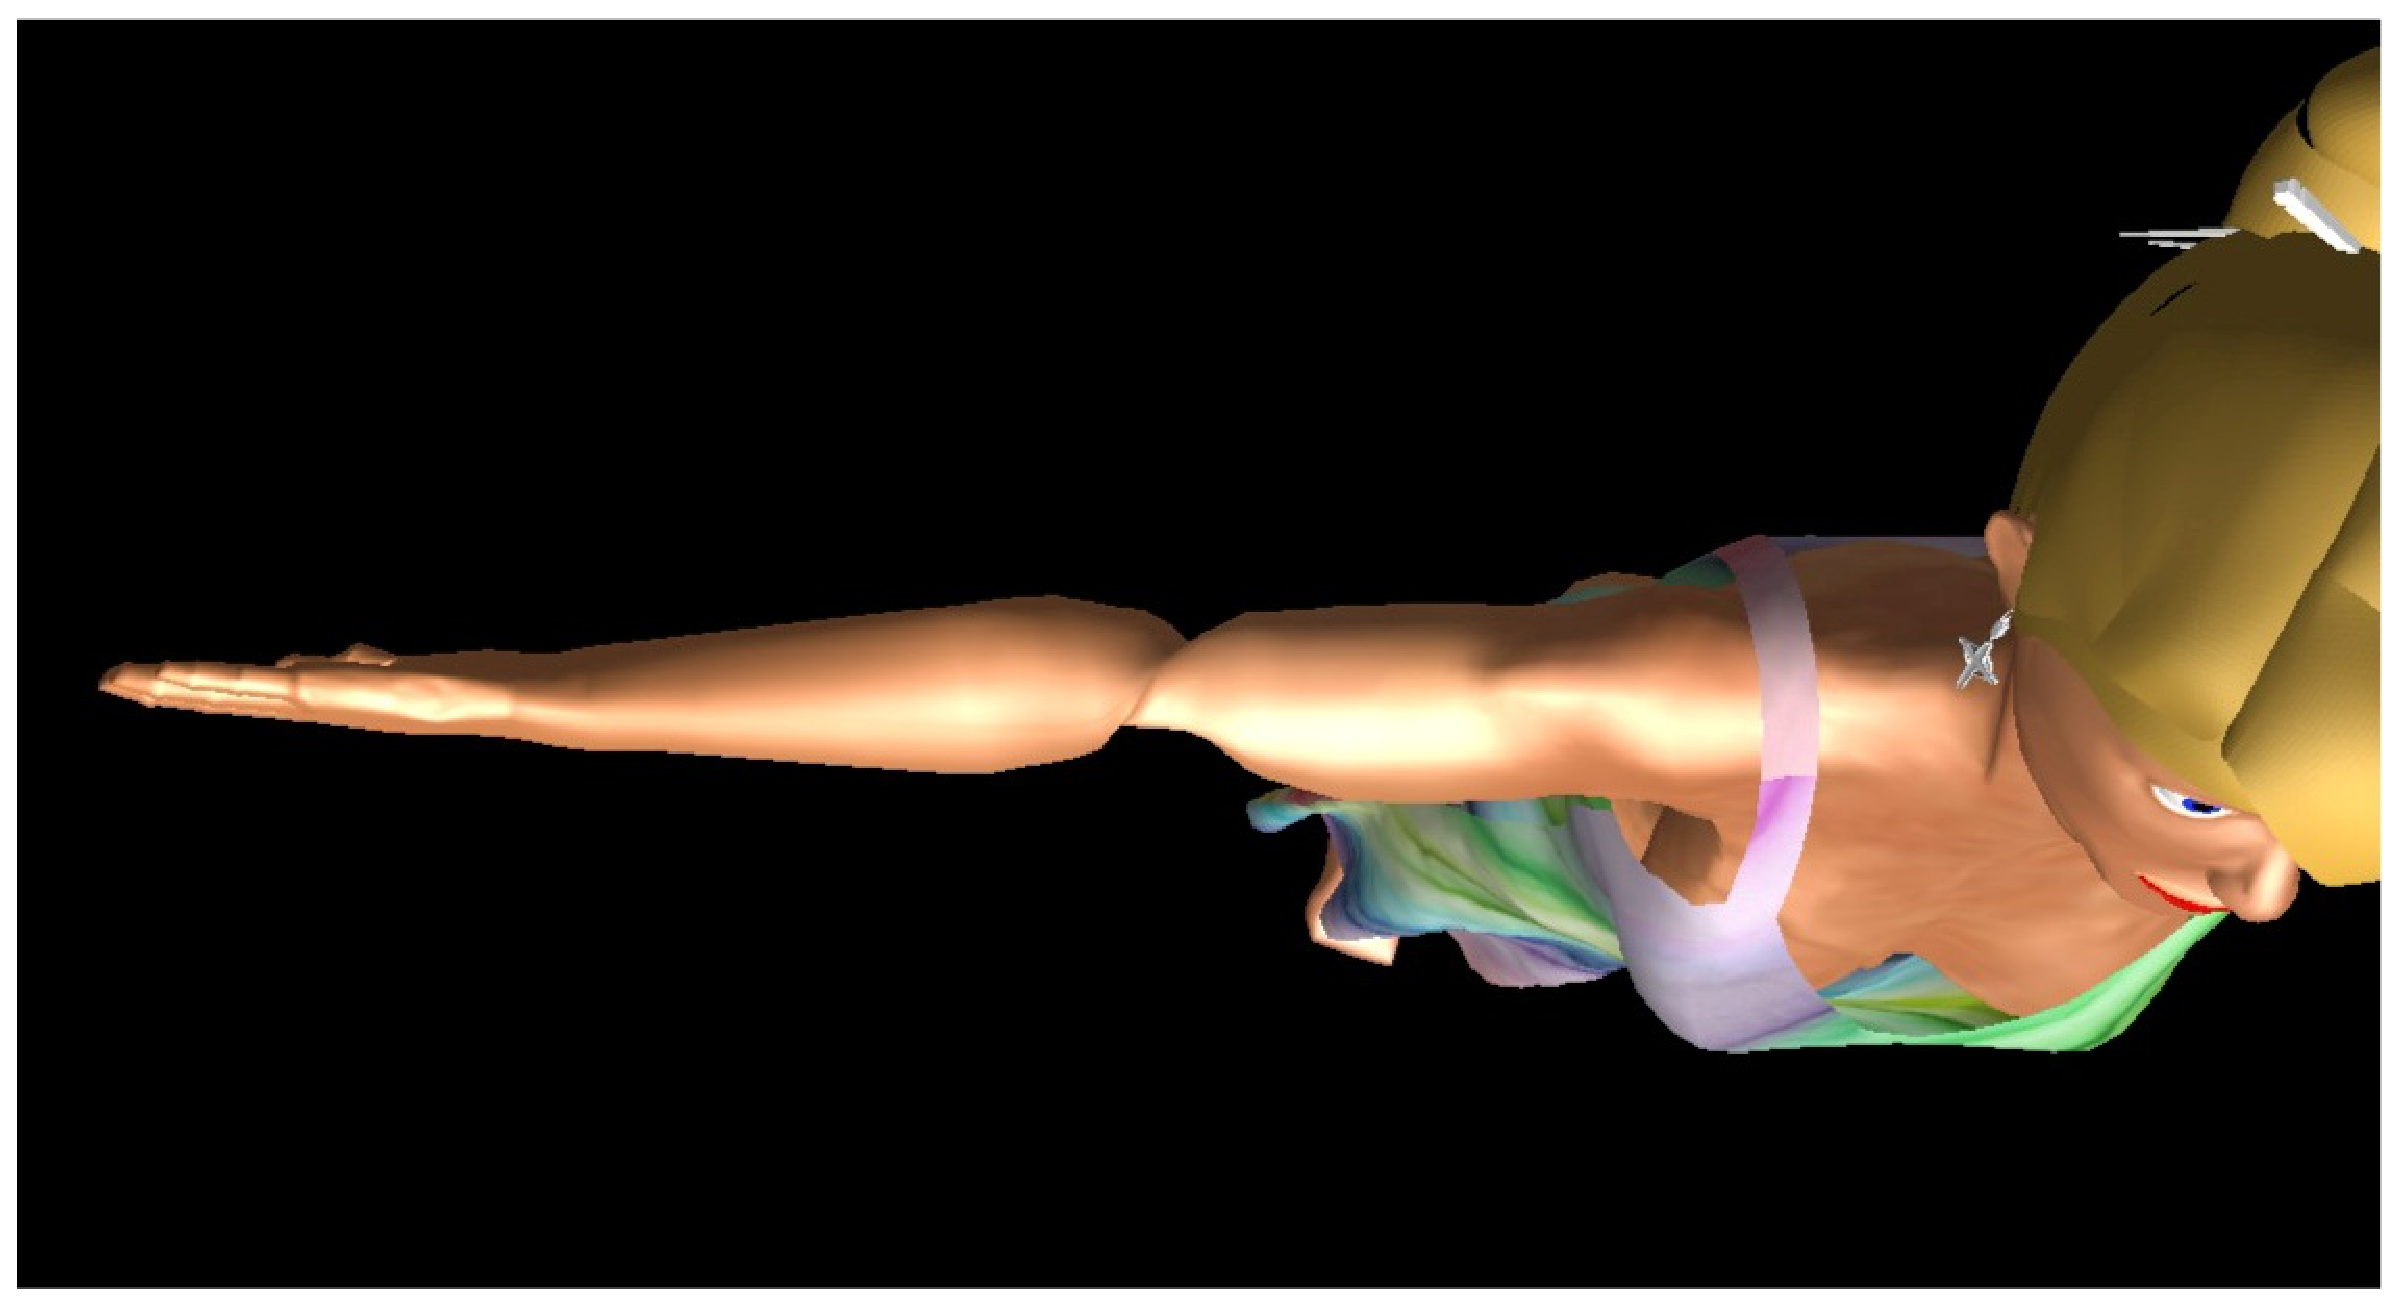
\includegraphics[width=1.0\columnwidth]{./figures/fore-arm-single-bone.eps}}
	\centerline{(a)}
	\centerline{\ }
	\centerline{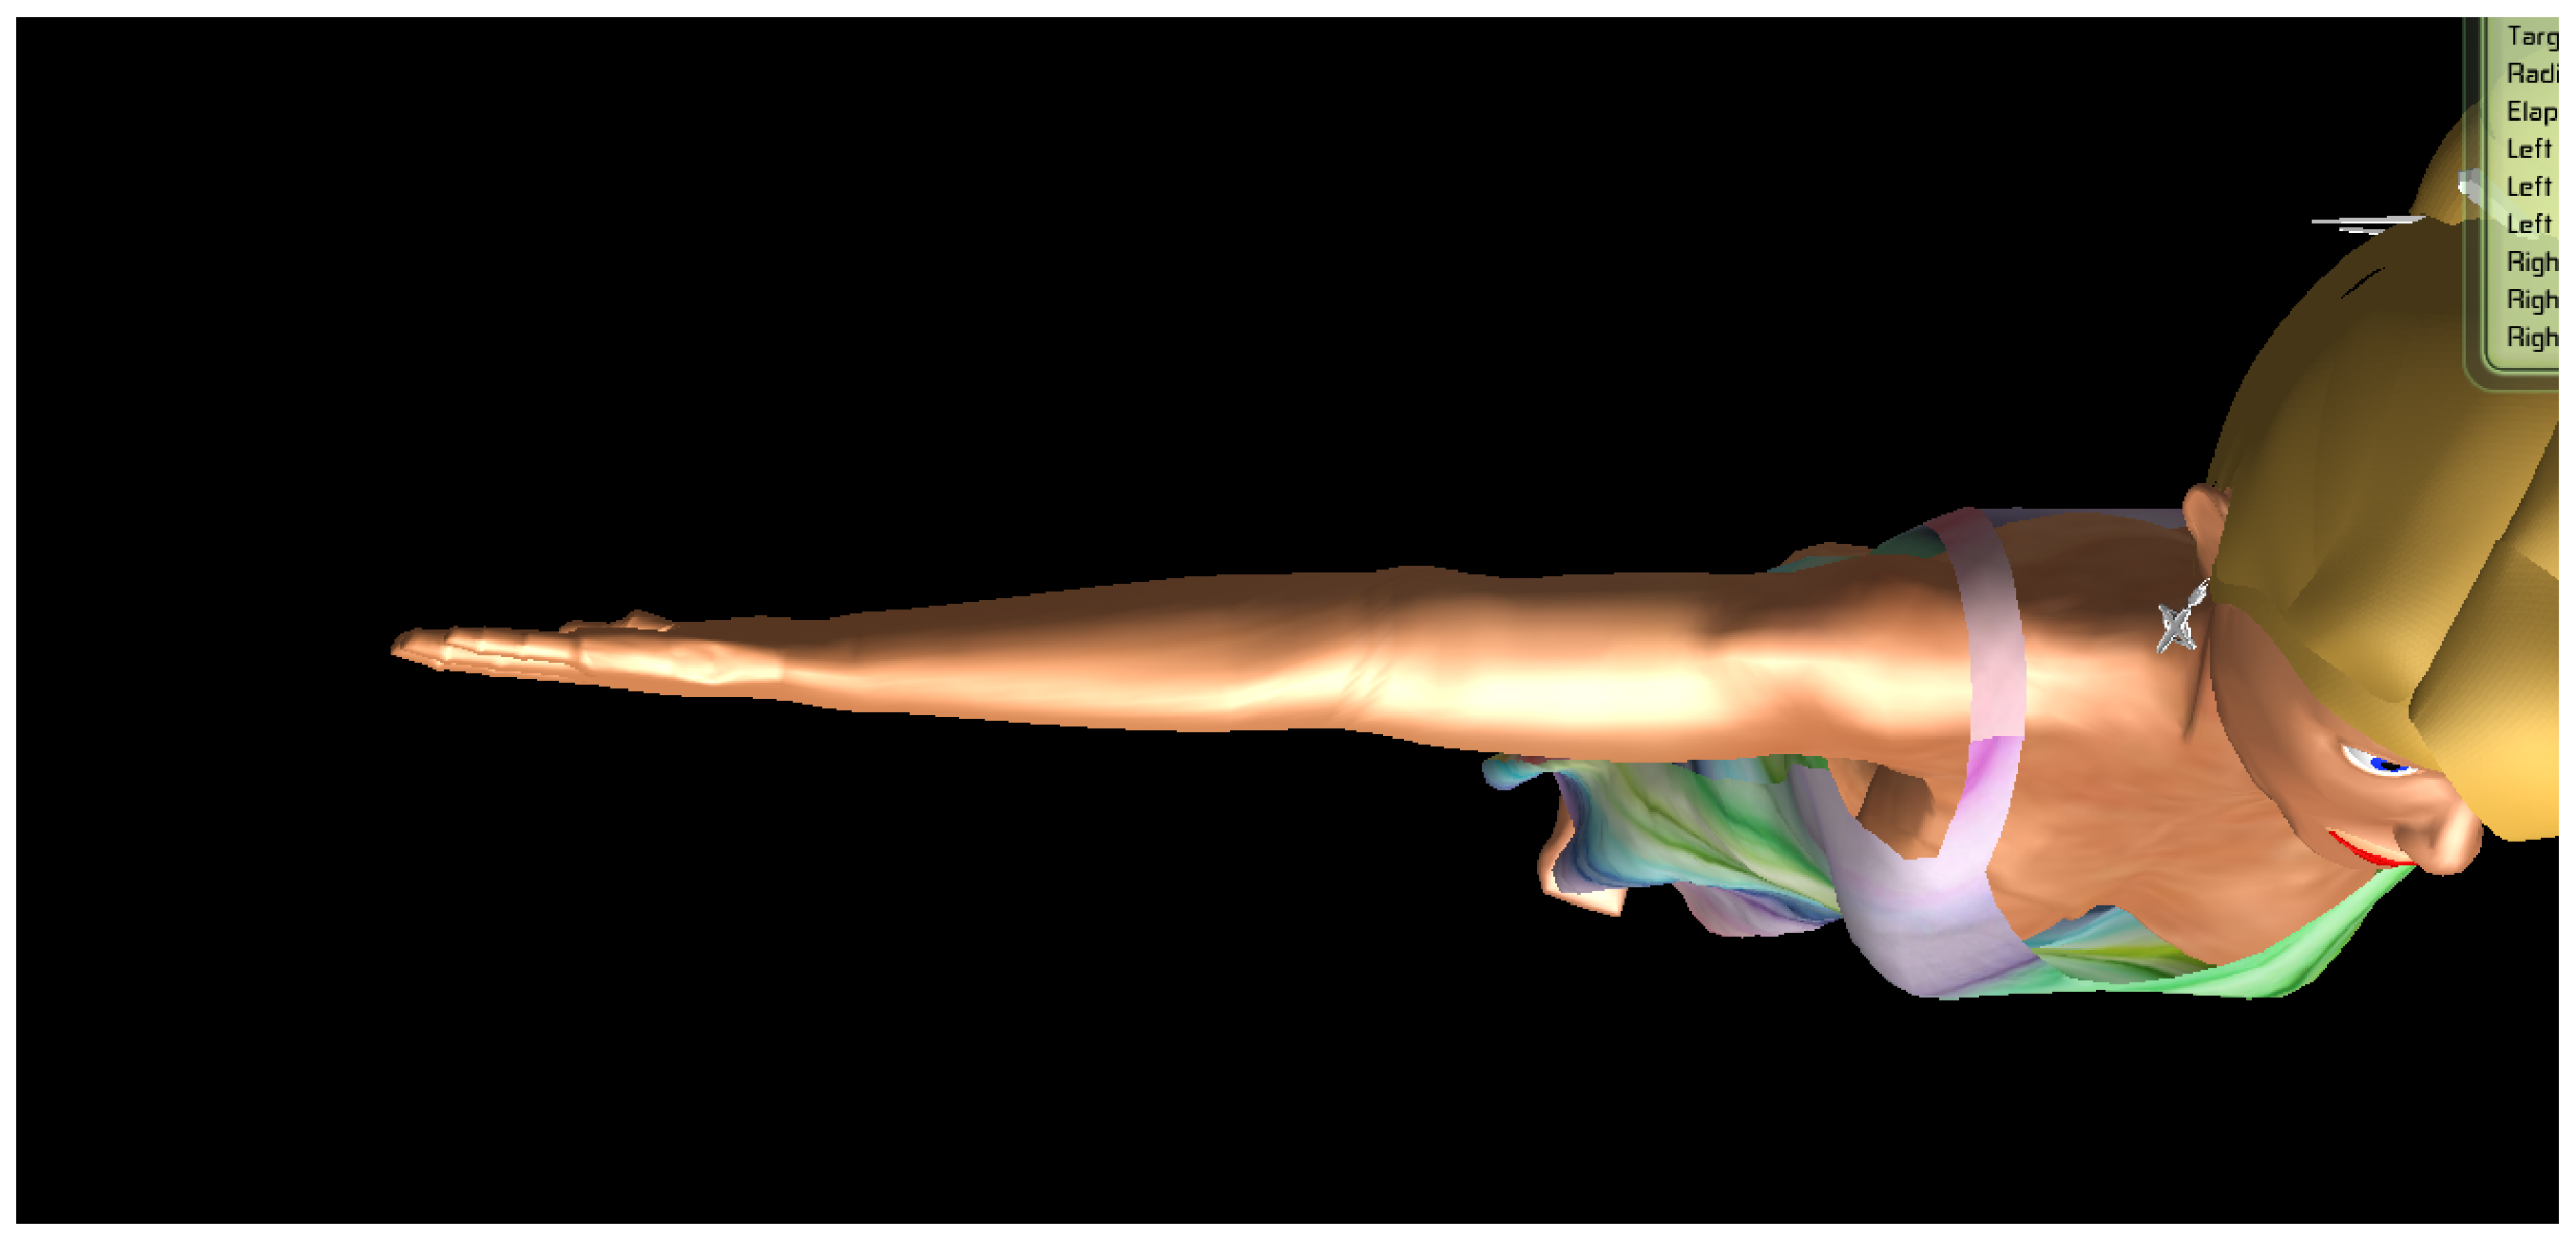
\includegraphics[width=1.0\columnwidth]{./figures/fore-arm-double-bone.eps}}
	\centerline{(b)}
	\caption{Comparison of a -90$^\circ$ yaw rotation on the forearm with: (a) single and (b)~double-boned skinning.}
	\label{fig:forearm-comparison}
\end{figure}

\subsubsection{Handling the Foot Skating Problem}
\label{section_foot_skating}
The virtual model is animated by changing bone orientations and root bone position. If the orientations and root position are applied to the bones respectively, the feet of the character appear to be floating on the ground that deteriorates the realism. 
This problem, known as footskating, is not limited to depth sensor applications. It shows up in motion-capture-based animation systems and solved in a reasonable way with approaches, such as Kovar et al.~\cite{Kovar2002} and Ikemoto et al.~\cite{Ikemoto2006}. However, these methods rely on some sort of preprocessing or supervised learning, which is not suitable for our system, as the motion is captured and applied im real time. Hence, a solution that does not require a training process is needed for such applications. Mankyu and Choi~\cite{Mankyu2013} propose a similar method that does not require training for real-time depth sensor applications. Their approach is adopted into our framework to overcome the footskating problem. However, it requires additional filters and constraints in order to be usable in our framework. It is assumed that one foot is always on the ground; otherwise, artifacts may occur, for example, if the user attempts jumping. The footskating handling algorithm consists of two parts: {\em constraint checking and adaptation} (cf.~Algorithm~\ref{algo:check_foot_constraints}) and {\em joint angle determination and application} (cf.~Algorithm~\ref{algo:foot_skating}). The whole   algorithm consists of the following four steps. 

\begin{enumerate}
\item Determine which foot is constrained by checking speed and location thresholds. The thresholds are changed adaptively in order to compensate for different sensor and user placements.

\item Place the constrained foot at its last recorded position and solve the inverse kinematics problem to determine the orientations of the hip and knee joints. Solving an inverse kinematic problem is no trivial task. There are various numerical and analytical methods for inverse kinematic problems and many implementations focusing on each. We use the IKAN library by University of Pennsylvania~\cite{IKAN2013}, which uses the approach described in~\cite{Tolani2000}.  

\item Check if the foot coincides with its intended position after the inverse kinematic orientations are applied to the bones. If there is a positional mismatch, relocate the root joint to complete alignment.

\item Smooth the joint orientation difference in order to avoid jumps from frame to frame. This is especially important when the constraint switches, as the source of the orientations are different in two cases and they do not always overlap. Smoothing parameters are optimized using trial and error; they are not viable for adaptive nature. Smoothing also helps to overcome the self-occlusion and data-noisiness.
\end{enumerate}
  
\begin{algorithm}[ht]
\DontPrintSemicolon % Some LaTeX compilers require you to use \dontprintsemicolon instead
\If{\textit{isFirstFrame}}{
\If{$p^y_{left} < p^y_{right}$ }{
	\textit{constrained = left}\;
	$y_\textit{threshold}=p^y_\textit{left}$\;
}
\Else {
	\textit{constrained = right}\;
	$y_\textit{threshold}=p^y_\textit{right}$\;
}
}

\If{$constrained is left$}{
	\tcc{Check if constraints still hold}
	\If{$p^y_\textit{left} > y_\textit{threshold} \;\; and \;\; v_\textit{left} > v_\textit{threshold}$}{
		\tcc{Foot is not constrained anymore, check other foot}
		\If{$p^y_\textit{right} > y_\textit{threshold} \;\;and\;\; v_\textit{right} > v_\textit{threshold}$}{
			\tcc{Neither foot are constrained}
			\textit{updateThresholds()} \tcc*[f]{Thresholds should be updated} 
			\textit{restart}\;
		}
		\Else(\tcc*[f]{Right foot is constrained, feet switched}){		
			\textit{constrained=right}\;
			\textit{recordRightFootPosition()}\;
			\textit{constraintSwitched = True}\;
		}
	} 
}
\Else{ 
	\tcc{Check if constraints still hold} 
	\If{$p^y_{\textit{right}} > y_{\textit{threshold}} \;\;and\;\; v_{\textit{right}} > v_{\textit{threshold}}$}{
		\tcc{Foot is not constrained anymore, check other foot}
		\If{$p^y_\textit{left} > y_\textit{threshold} \;\;and\;\; v_\textit{left} > v_\textit{threshold}$}{
			\tcc{Neither foot are constrained}
			\textit{updateThresholds()} \tcc*[f]{Thresholds should be updated} 
			\textit{restart}\;
		} 
		\Else (\tcc*[f]{Left foot is constrained, feet switched}){	
			\textit{constrained = left}\;
			\textit{recordRightFootPosition()}\;
			\textit{constraintSwitched = True}\;
		}
	} 
}
\caption{Constrained foot determination}
\label{algo:check_foot_constraints}
\end{algorithm}

 
\begin{algorithm}[ht]
\DontPrintSemicolon % Some LaTeX compilers require you to use \dontprintsemicolon instead
{\textit checkFootConstraints()} \tcc*[f]{Check which foot is constrained}
$p^{\textit{foot}}_{\textit{constrained}} = {\textit getRecordedFootPosition()}$\;
${\textit{target}}_{ik} = p^{\textit{foot}}_{\textit{constrained}} - p^{\textit{hip}}_{\textit{constrained}}$\;
\tcc{Get the rotation quaternions for constrained hip and knee}
$q_{\textit{hip}}, q_{\textit{knee}}$ =  \textit{solveIkan}(\textit{constrained}, {\textit{target}}$_{ik}$)\;
${\textit{hip}}_{\textit{constrained}}.{\textit{rotate}}(q_{\textit{hip}})$\;
${\textit{foot}}_{\textit{constrained}}.{\textit{rotate}}(q_{\textit{hip}})$\;
$p^{\textit{foot}}_{\textit{new}} = {\textit{calculateForwardKinematics()}}$\;
\tcc{Calculate the root displacement vector}
$d_{{\textit{root}}}$ = $p^{\textit{foot}}_{\textit{constrained}}$ - $p^{\textit{foot}}_{\textit{new}}$\;
\textit{root}.\textit{translate}(d$_{\textit{root}}$)\;
\tcc{Proceed with joint smoothing}
\caption{Foot skating filtering}
\label{algo:foot_skating}
\end{algorithm}

Joint smoothing consists of interpolating between frames, especially when there is a significant change in orientations, which would normally cause a non-continuous animation. Old joint orientations are always recorded in the global coordinate system and updated everyframe. After we get the new orientation from the new frame, we calculate the quaternion that would rotate the old orientation to the new one:

\begin{equation}
Q_{d} = Q_{new} \times Q_{old}^{-1}
\label{eqn:rotator_quaternion}
\end{equation} 

When we compute the delta quaternion, we get its axis-angle representation. Because we are interested in rotating the joint partially, we build up a new quaternion with the same axis and a fraction of the same angle. The fraction varies with whether the constraint is switched recently. 

\begin{equation} 
\begin{split}
Q_{d} = \textit{Quaternion}((x, y, z), \alpha) \\  
Q_d^* = \textit{Quaternion}((x, y, z), \alpha / k )
\label{eqn:partial_rotator}
\end{split}
\end{equation} 

The fractional rotations are then applied to the joints to get a smoother movement. Other implicit operations include coordinate system transformations, as we are working with three different coordinate systems: Global-Render Coordinate System, Local-Render Coordinate System, and IKAN Coordinate System. 
%The constraints of the IKAN library require certain to-and-from transformations to be applied with the coordinate systems. 

\section{Experiments}
\label{sec:Experiments}
The proposed depth map enhancement algorithm is implemented on the in-house developed virtual dressing software, which acts as 
the test bench for experimentation. The measurement process to identify the body parameters starts after a subject is recognized,
identified and calibrated for tracking. Following the parameter estimation, the virtual avatar and cloth are created and the 
simulation starts.

Experiments are performed on a high-end PC with Intel i7-2600 and NVIDIA GeForce GTX560Ti. The total time for the measurement of body parameters and 
resizing the cloth does not exceed 1.005 seconds. Considering the time for acquiring 30 frames of input from the depth sensor is 1.0 second, it is safe to say that the measurement algorithm does not introduce any delays for a real time application because it needs to run only once at the beginning of the simulation. The actual simulation runs at 600 fps on $1920 \times 1080$ resolution. The body sizes are estimated with error rates less than 4\%, which is sufficient for the realism of the simulation and determining the appropriate apparel size. 

Two sets of frame rates across the simulation can be seen in Figure~\ref{fig:fps}. Notice the common pattern in both of the simulations. The first drop corresponds to the start of the animation of the avatar with the input from depth sensor. Until that point, the avatar is static, the motion filters do not run and the simulation runs at a higher speed. Approximately 600 fps is lost due to the motion filtering and skinning. The first cliff in the graph corresponds to the point where the physics simulation is stopped. The second cliff starts when the input from the depth sensor is stopped and the simulation is stagnant.  

\begin{figure}[htbp]
	\begin{center} 
	\fbox{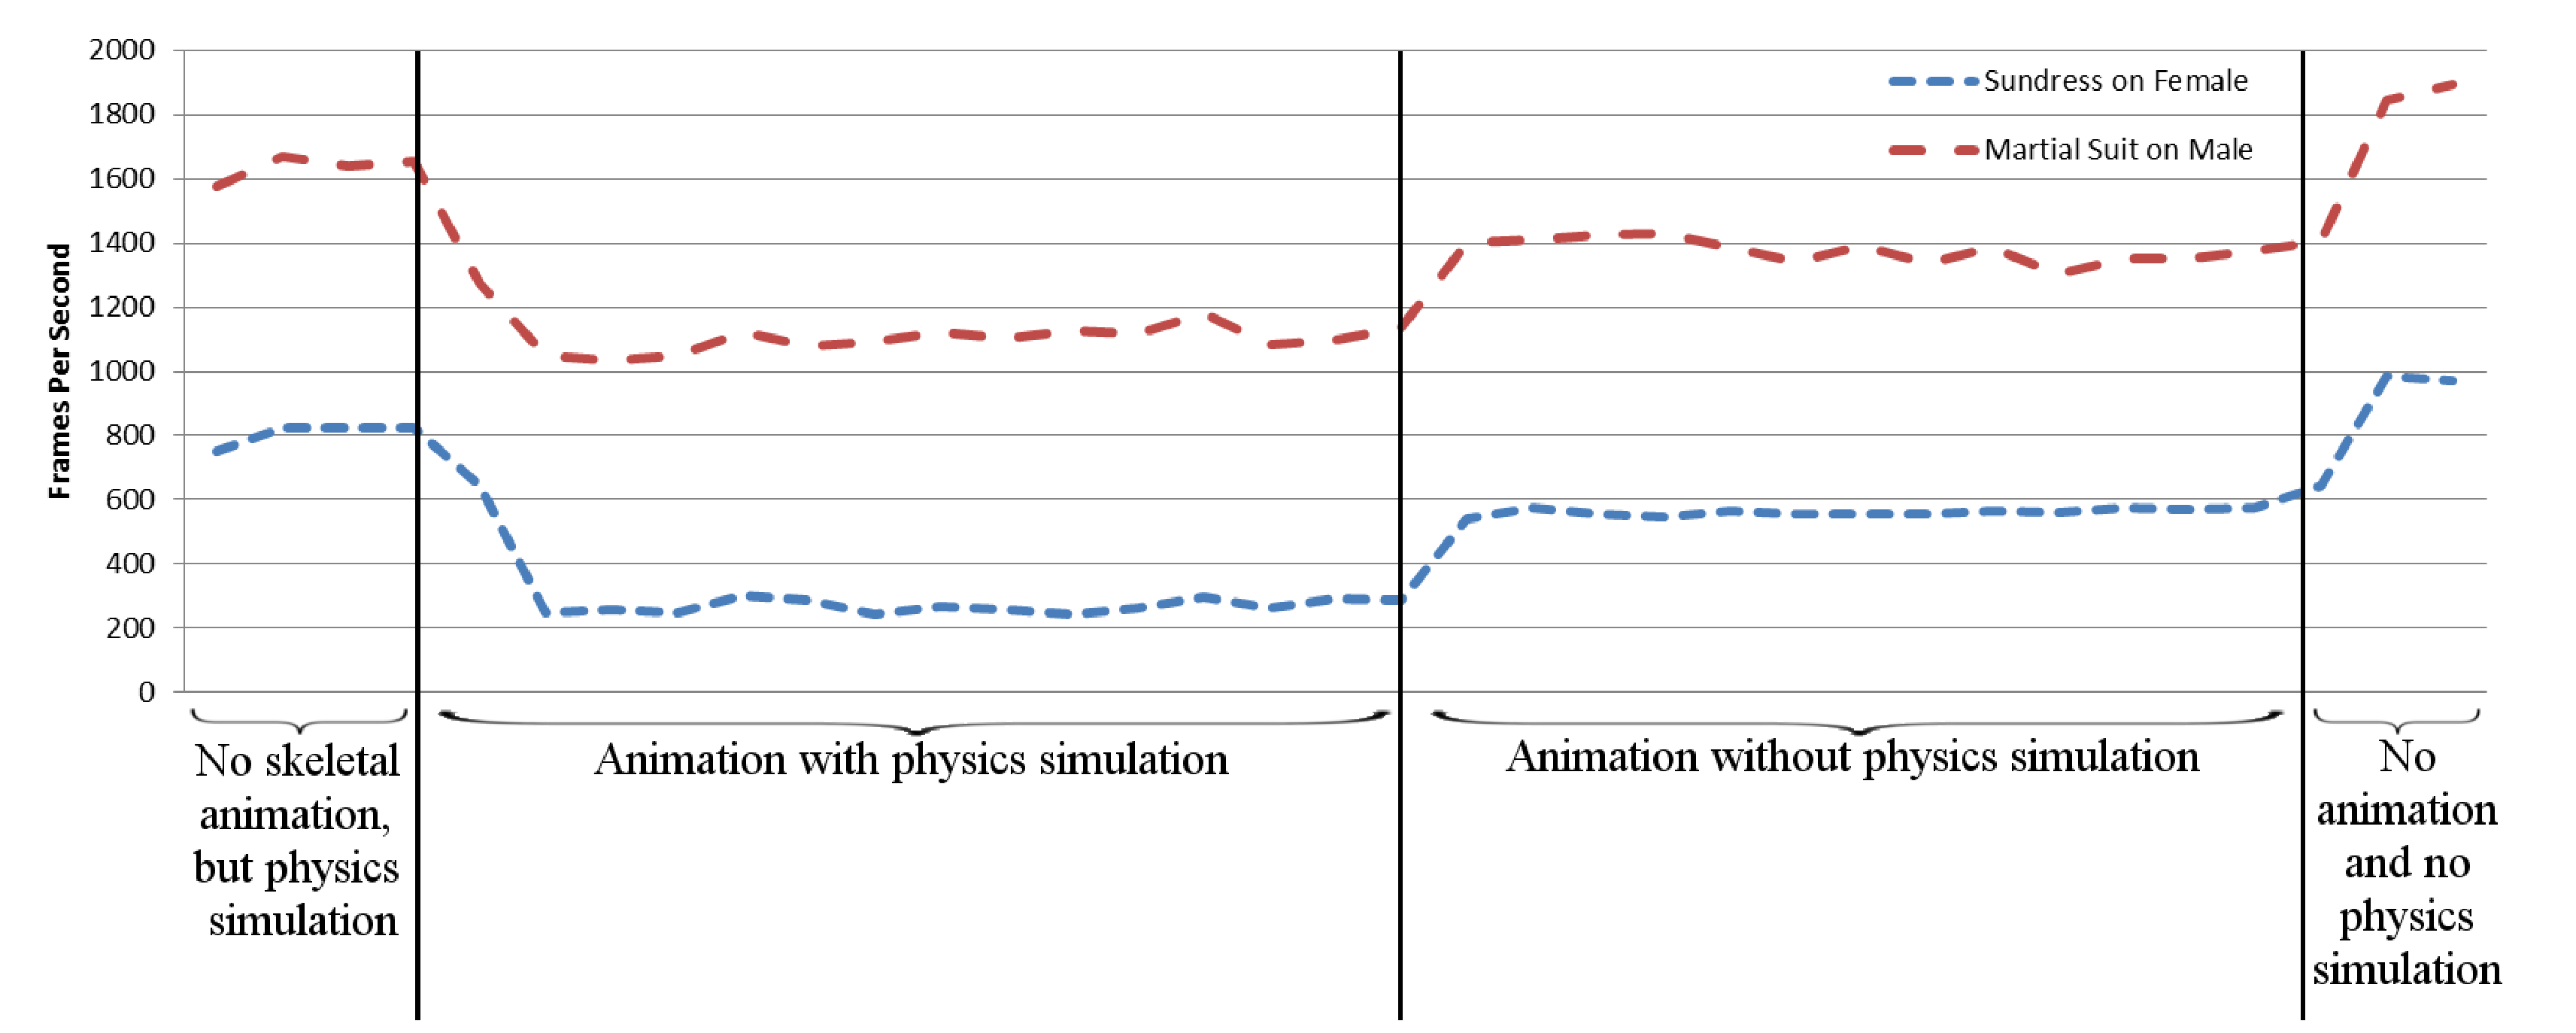
\includegraphics[width=0.98\textwidth]{./figures/fps.eps}}
	\end{center}
	\caption{The frame rates for two different apparel meshes. }
	\label{fig:fps}
\end{figure}

The filters on the legs focus on solving the foot skating problem. The corrected displacement values can be seen in Figure~\ref{fig:footskating}. The virtual unit is the unit step in the virtual world. For reference, the virtual avatars' height is 55 virtual units. Hence, a virtual unit corresponds close to 3.5 cm.  

\begin{figure}[htbp] 
	\begin{center} 
	\fbox{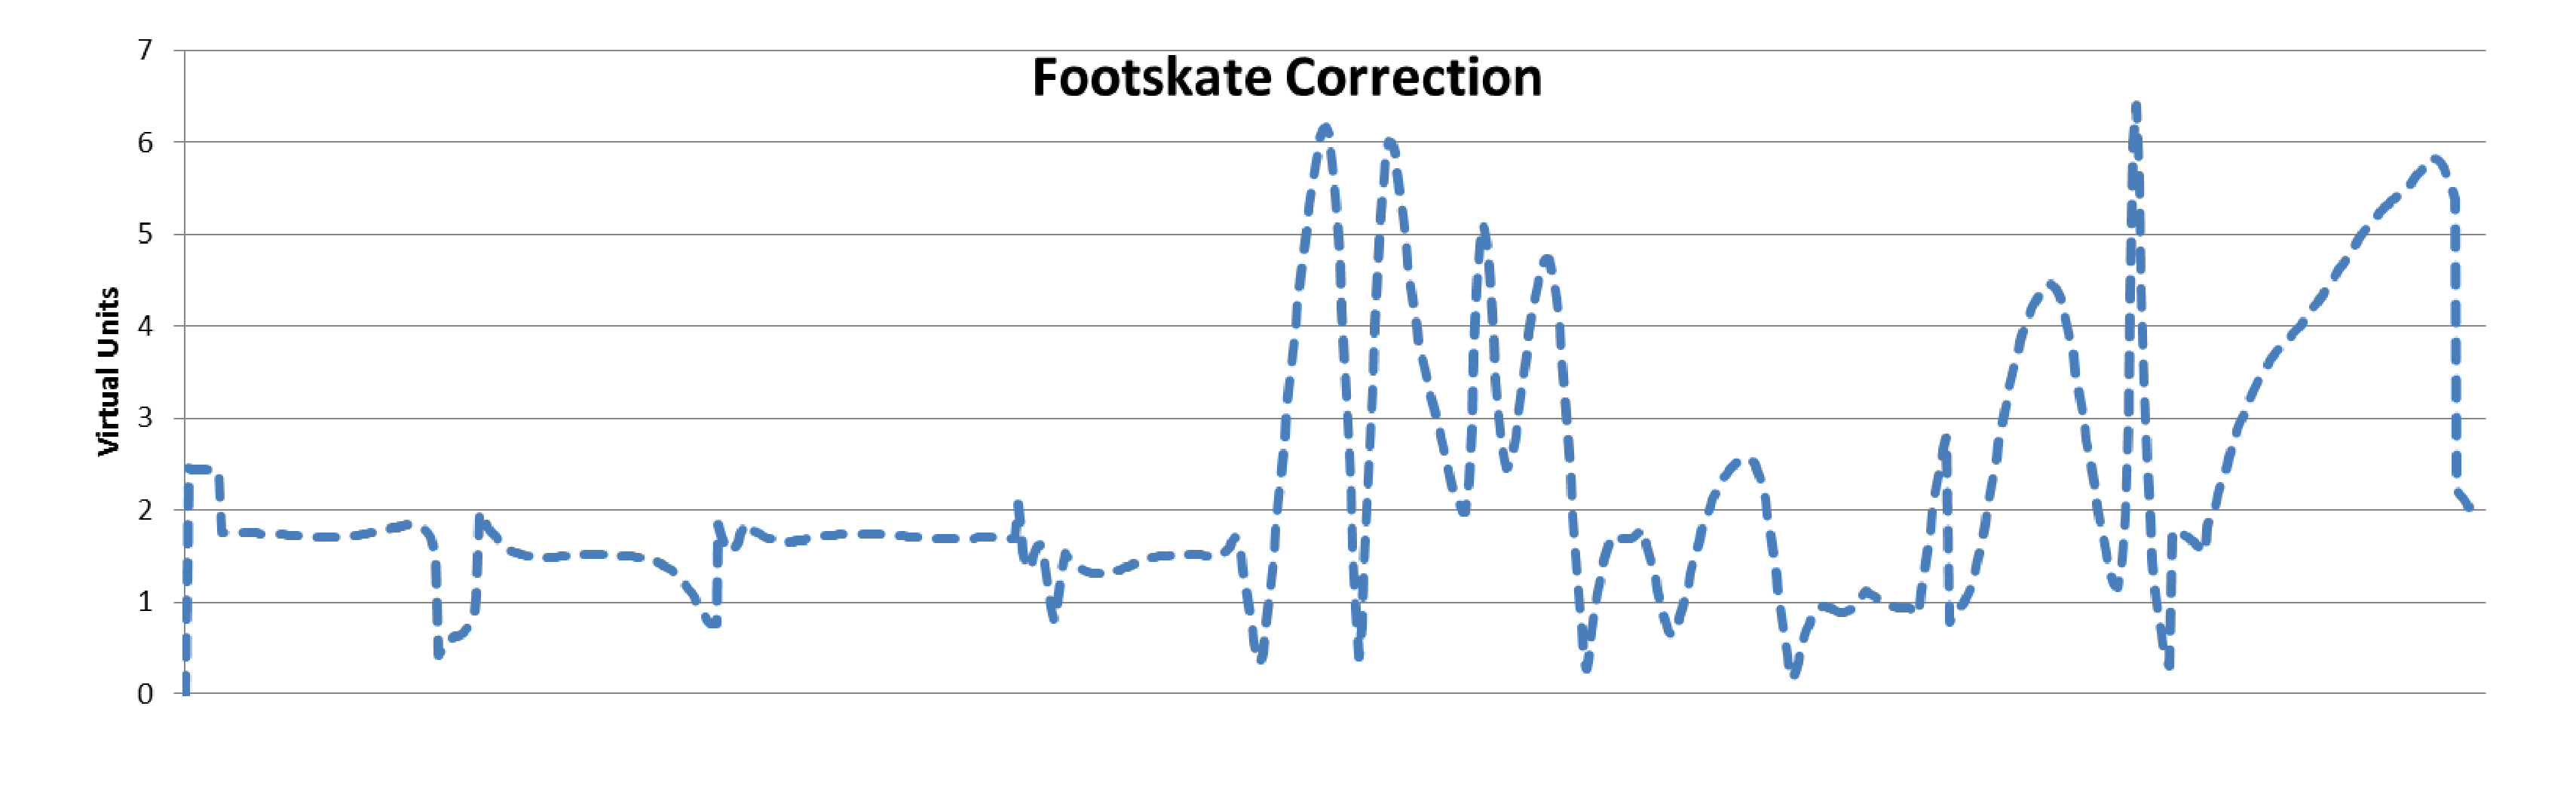
\includegraphics[width=0.98\textwidth]{./figures/footskate.eps}}
	\end{center}
	\caption{The corrected displacement of feet. The local minima correspond to constrained foot changes and subsequent 
	position smoothing. The zig zag regions correspond to time intervals where the user performing body yaw motion where 
	the foot are considerably sliding.}
	\label{fig:footskating}
\end{figure}

Table~\ref{tbl:body_results} presents the measurements of the body dimensions, as well as the errors and standard deviations of the measurements in 30 frames for three subjects. Our results are compared with the results from~\cite{Giovanni2012} and \cite{Samejima2012}, which are also real-time applications, in Table~\ref{tbl:performance_compare}.

\singlespacing

\begin{table}
\begin{center}
\begin{tabular}{|c|c|c|c|c|c|c|c|c|}
\hline
  & \multicolumn{4}{c|}{\textbf{Shoulder Width (cm)}} & \multicolumn{4}{c|}{\textbf{Body Height (cm)}} \\ \hline
  \rotatebox{90}{Subject } & \rotatebox{90}{Real } & \rotatebox{90}{Estimated } & \rotatebox{90}{Error (\%)} & \rotatebox{90}{Deviation } & \rotatebox{90}{Real } & \rotatebox{90}{Estimated } & \rotatebox{90}{Error (\%)} & \rotatebox{90}{Deviation } \\ \hline
 1 & 43 & 43.6 & 1.0 & 7.8 & 172 & 170.8 & 0.6 & 2.5  \\ \hline
 2 & 46 & 44.3 & 3.0 & 8.5 & 176 & 172.1 & 2.0 & 1.4  \\ \hline
 3 & 51 & 48.8 & 4.0 & 12.1 & 176 & 174.0 & 1.0 & 6.6  \\ \hline
 4 & 48 & 50.0 & 4.0 & 2.5 & 188 & 191.0 & 1.5 & 7.1  \\ \hline
 5 & 44 & 42.6 & 3.0 & 4.2 & 178 & 175.8 & 1.2 & 3.1  \\ \hline
\end{tabular}
\end{center}
\caption{Performance figures for five different subjects.}
\label{tbl:body_results}
\end{table} 



\begin{table}
\begin{center}
\begin{tabular}{|l|c|c|c|c|} 
\hline 
  & \rotatebox{90}{\parbox[c]{2.95cm}{\mbox{Error Average} \mbox{\hspace{0.7cm}(\%)}}} & \rotatebox{90}{\parbox[c]{2.95cm}{\mbox{Error Deviation} \mbox{\hspace{0.7cm}(\%)}}} & \rotatebox{90}{Duration} & \rotatebox{90}{Estimation} \\ \hline
  Our Approach & 2.13  & 1.20   & 1.00 & Fixed \\ \hline 
  Giovanni et al.~\cite{Giovanni2012}  & 4.00  & 3.00  & 1.00 & None \\ \hline
  Samejima et al.~\cite{Samejima2012}  & 6.72  & 4.68  & n/a & PCA \\ \hline
\end{tabular}
\end{center}  
\caption{Performance comparison with \cite{Giovanni2012} and \cite{Samejima2012} regarding height measurements.}
\label{tbl:performance_compare}
\end{table}

\doublespacing

For the collision spheres, the quality of the results can be assessed by the smoothness of the collision simulation, as seen in Figure \ref{fig:system}. Throughout the simulation, unnatural intersections between the cloth and the avatar never take place, while the cloth appears to rest on the skin naturally, without space between the two meshes. Figure~\ref{fig:examples} shows examples of three garments on a model with different postures generated with our implementation. 

\begin{figure}[htbp]
	\begin{center} 
			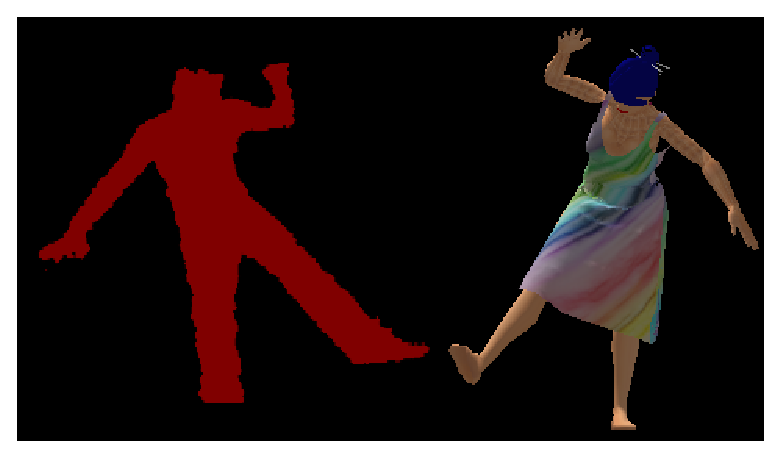
\includegraphics[width=1.00\textwidth]{./figures/scshot.eps}
	\end{center}
	\caption{An example depth map data and the corresponding posture of the subject with a virtual cloth on it.}
	\label{fig:system}
\end{figure}
 
 \begin{figure}[htbp] 
	\centerline{
	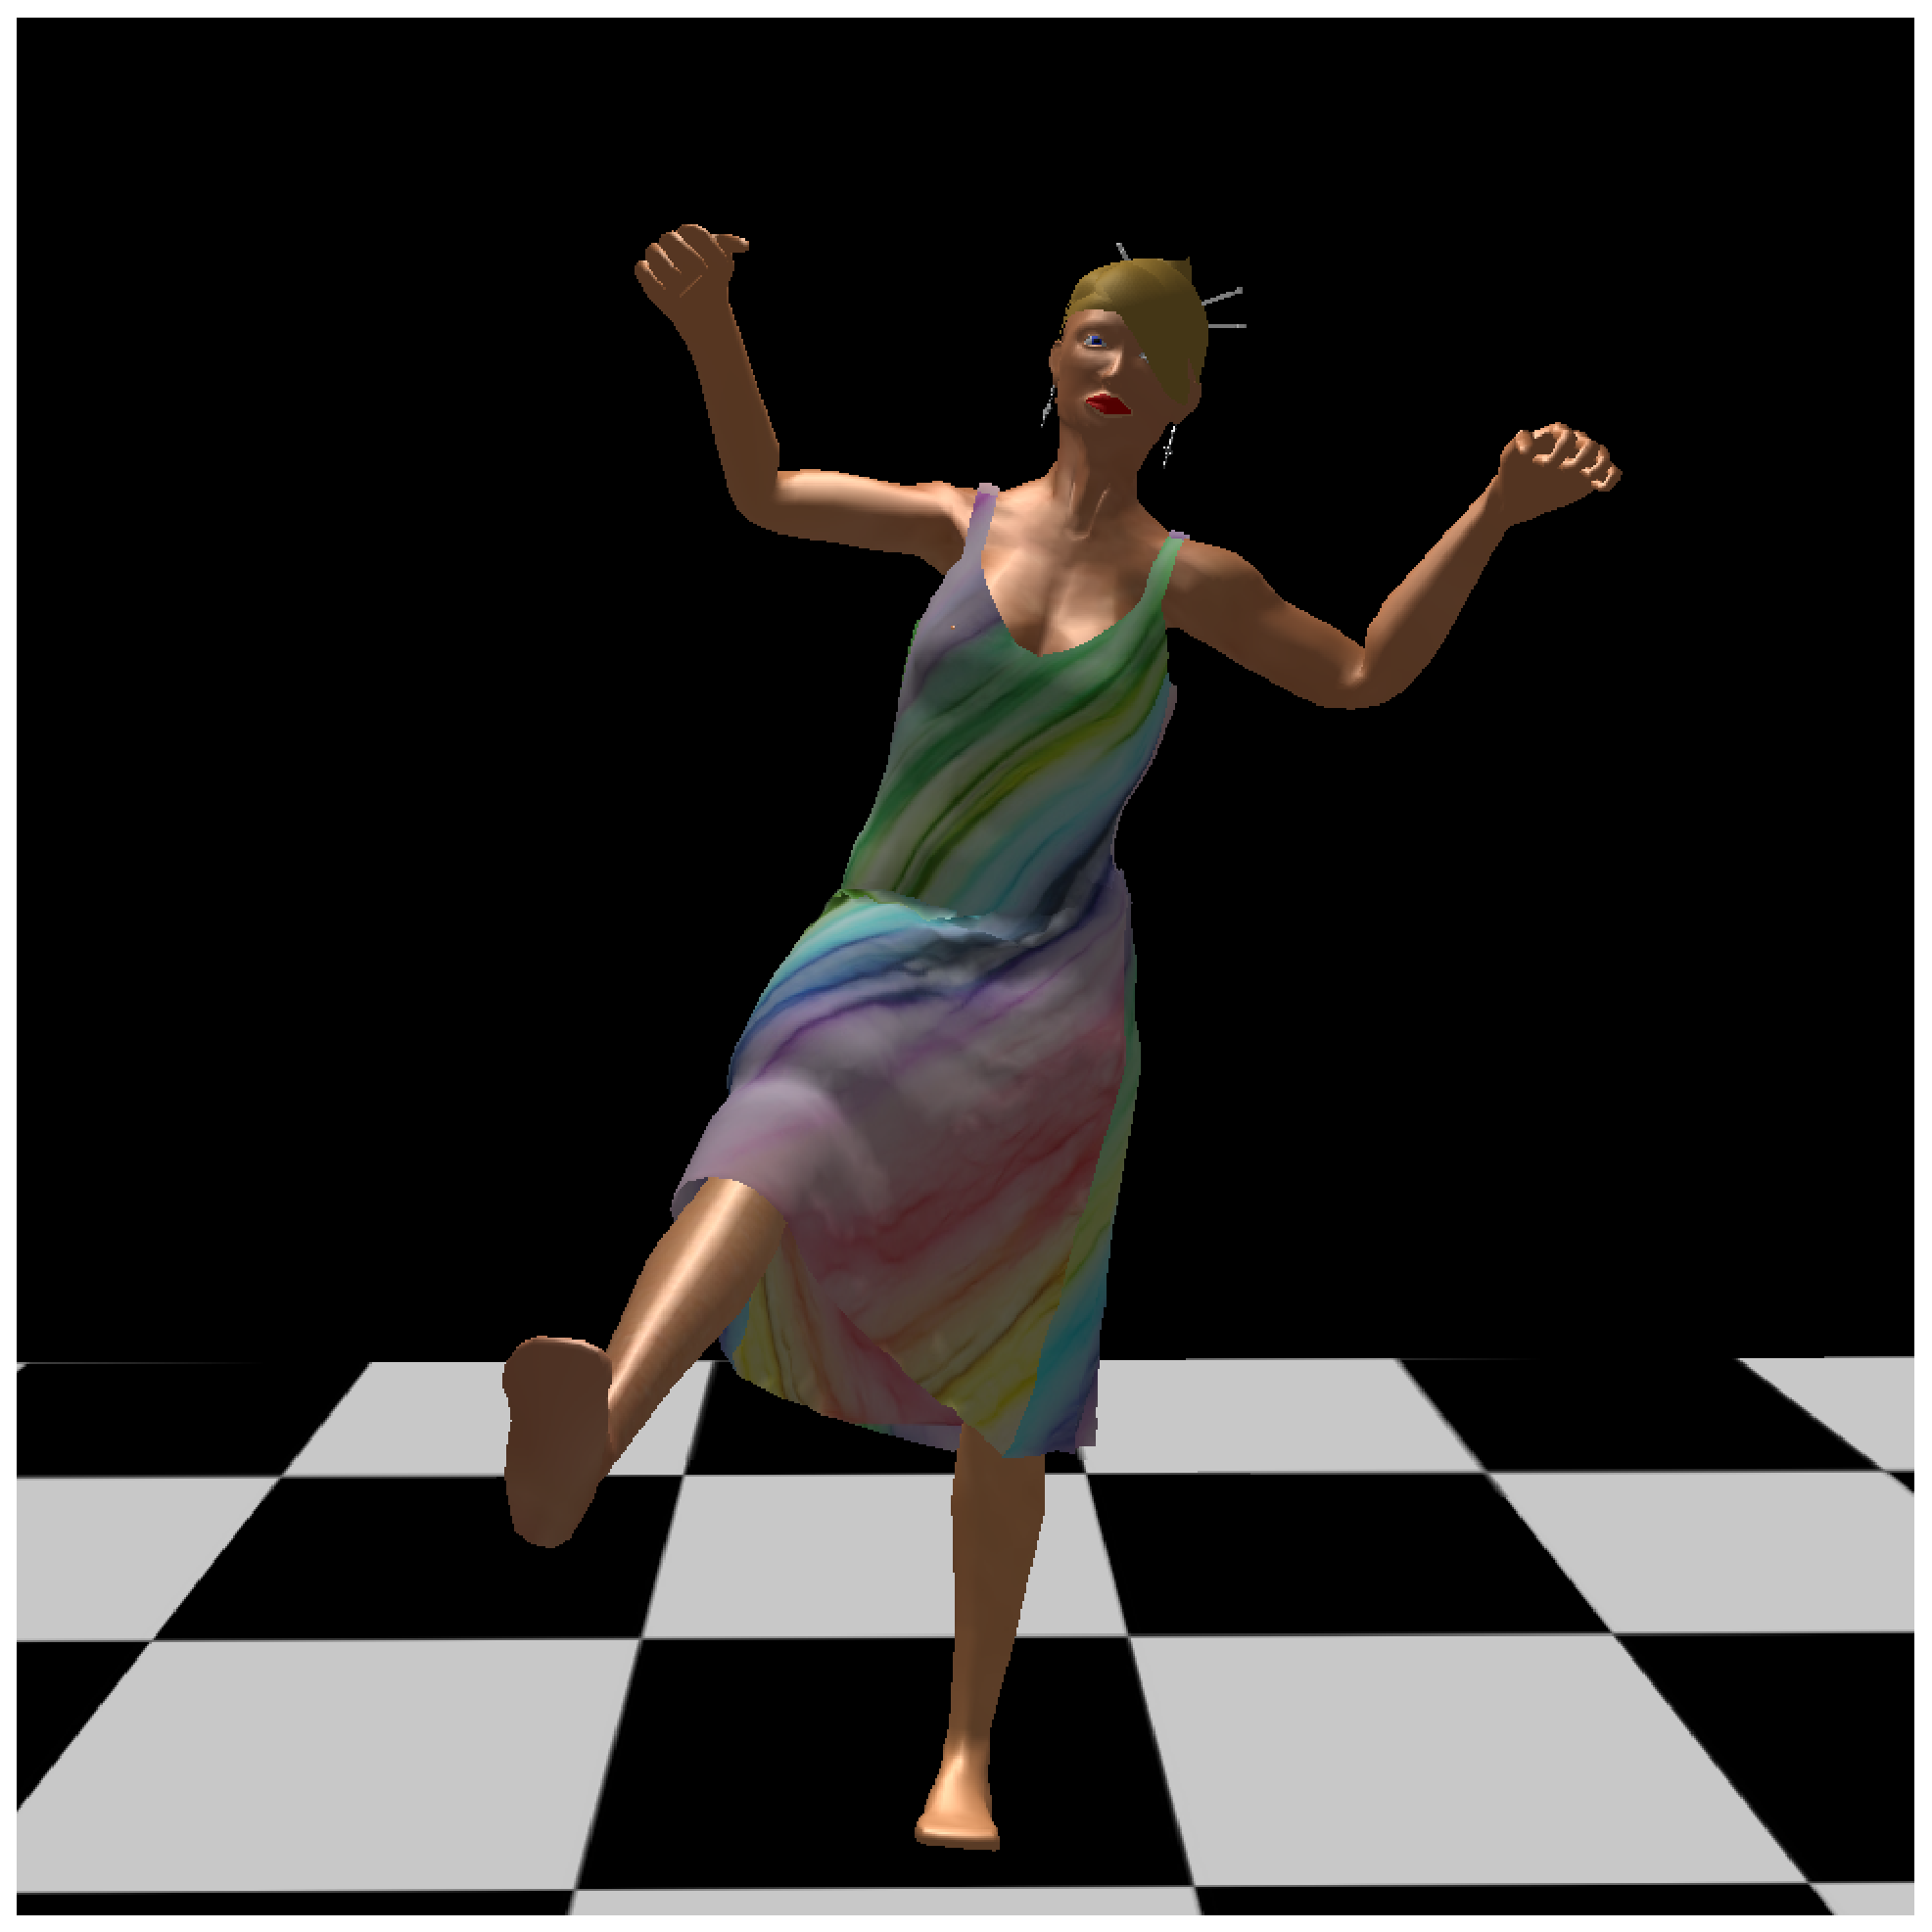
\includegraphics[width=0.250\textwidth]{./figures/sundress1.eps}
	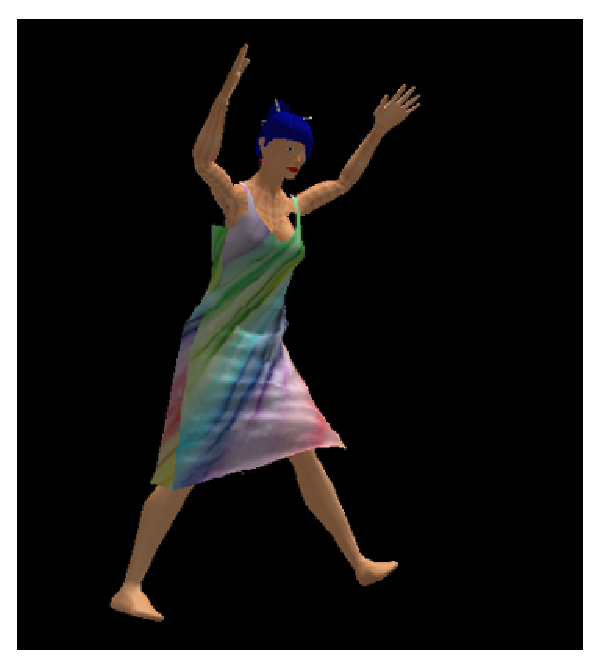
\includegraphics[width=0.250\textwidth]{./figures/sundress2.eps}
	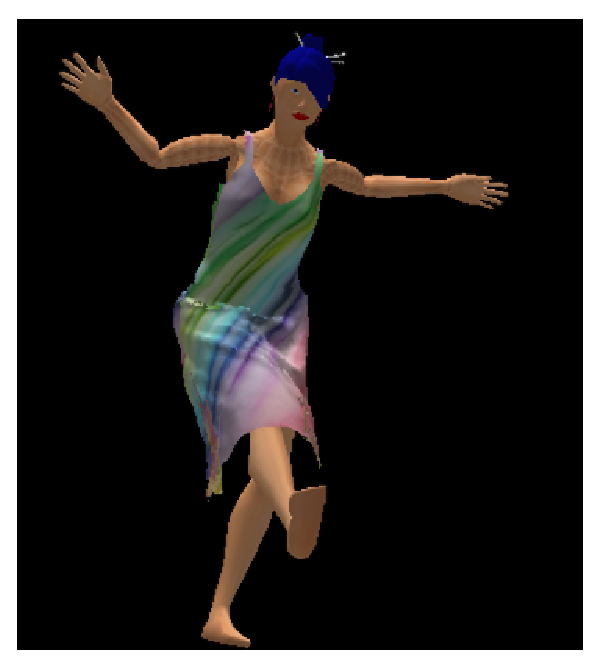
\includegraphics[width=0.250\textwidth]{./figures/sundress3.eps}
	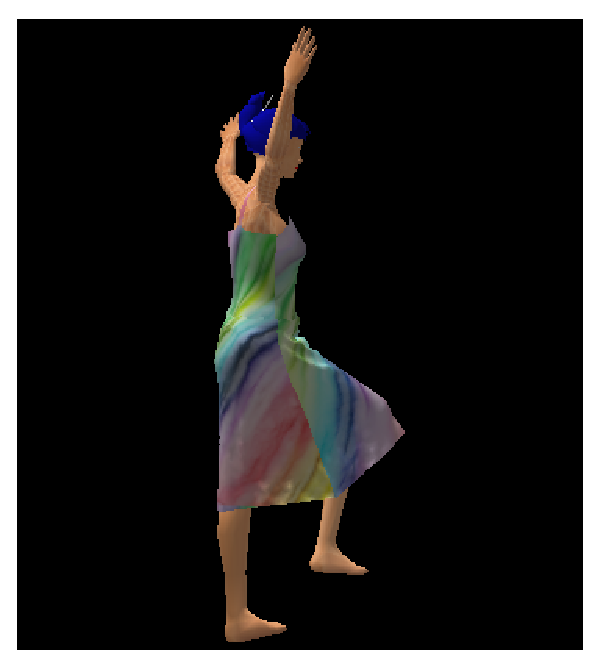
\includegraphics[width=0.250\textwidth]{./figures/sundress4.eps}
	}
	\centerline{(a)}
	\centerline{\ }
	\centerline{
	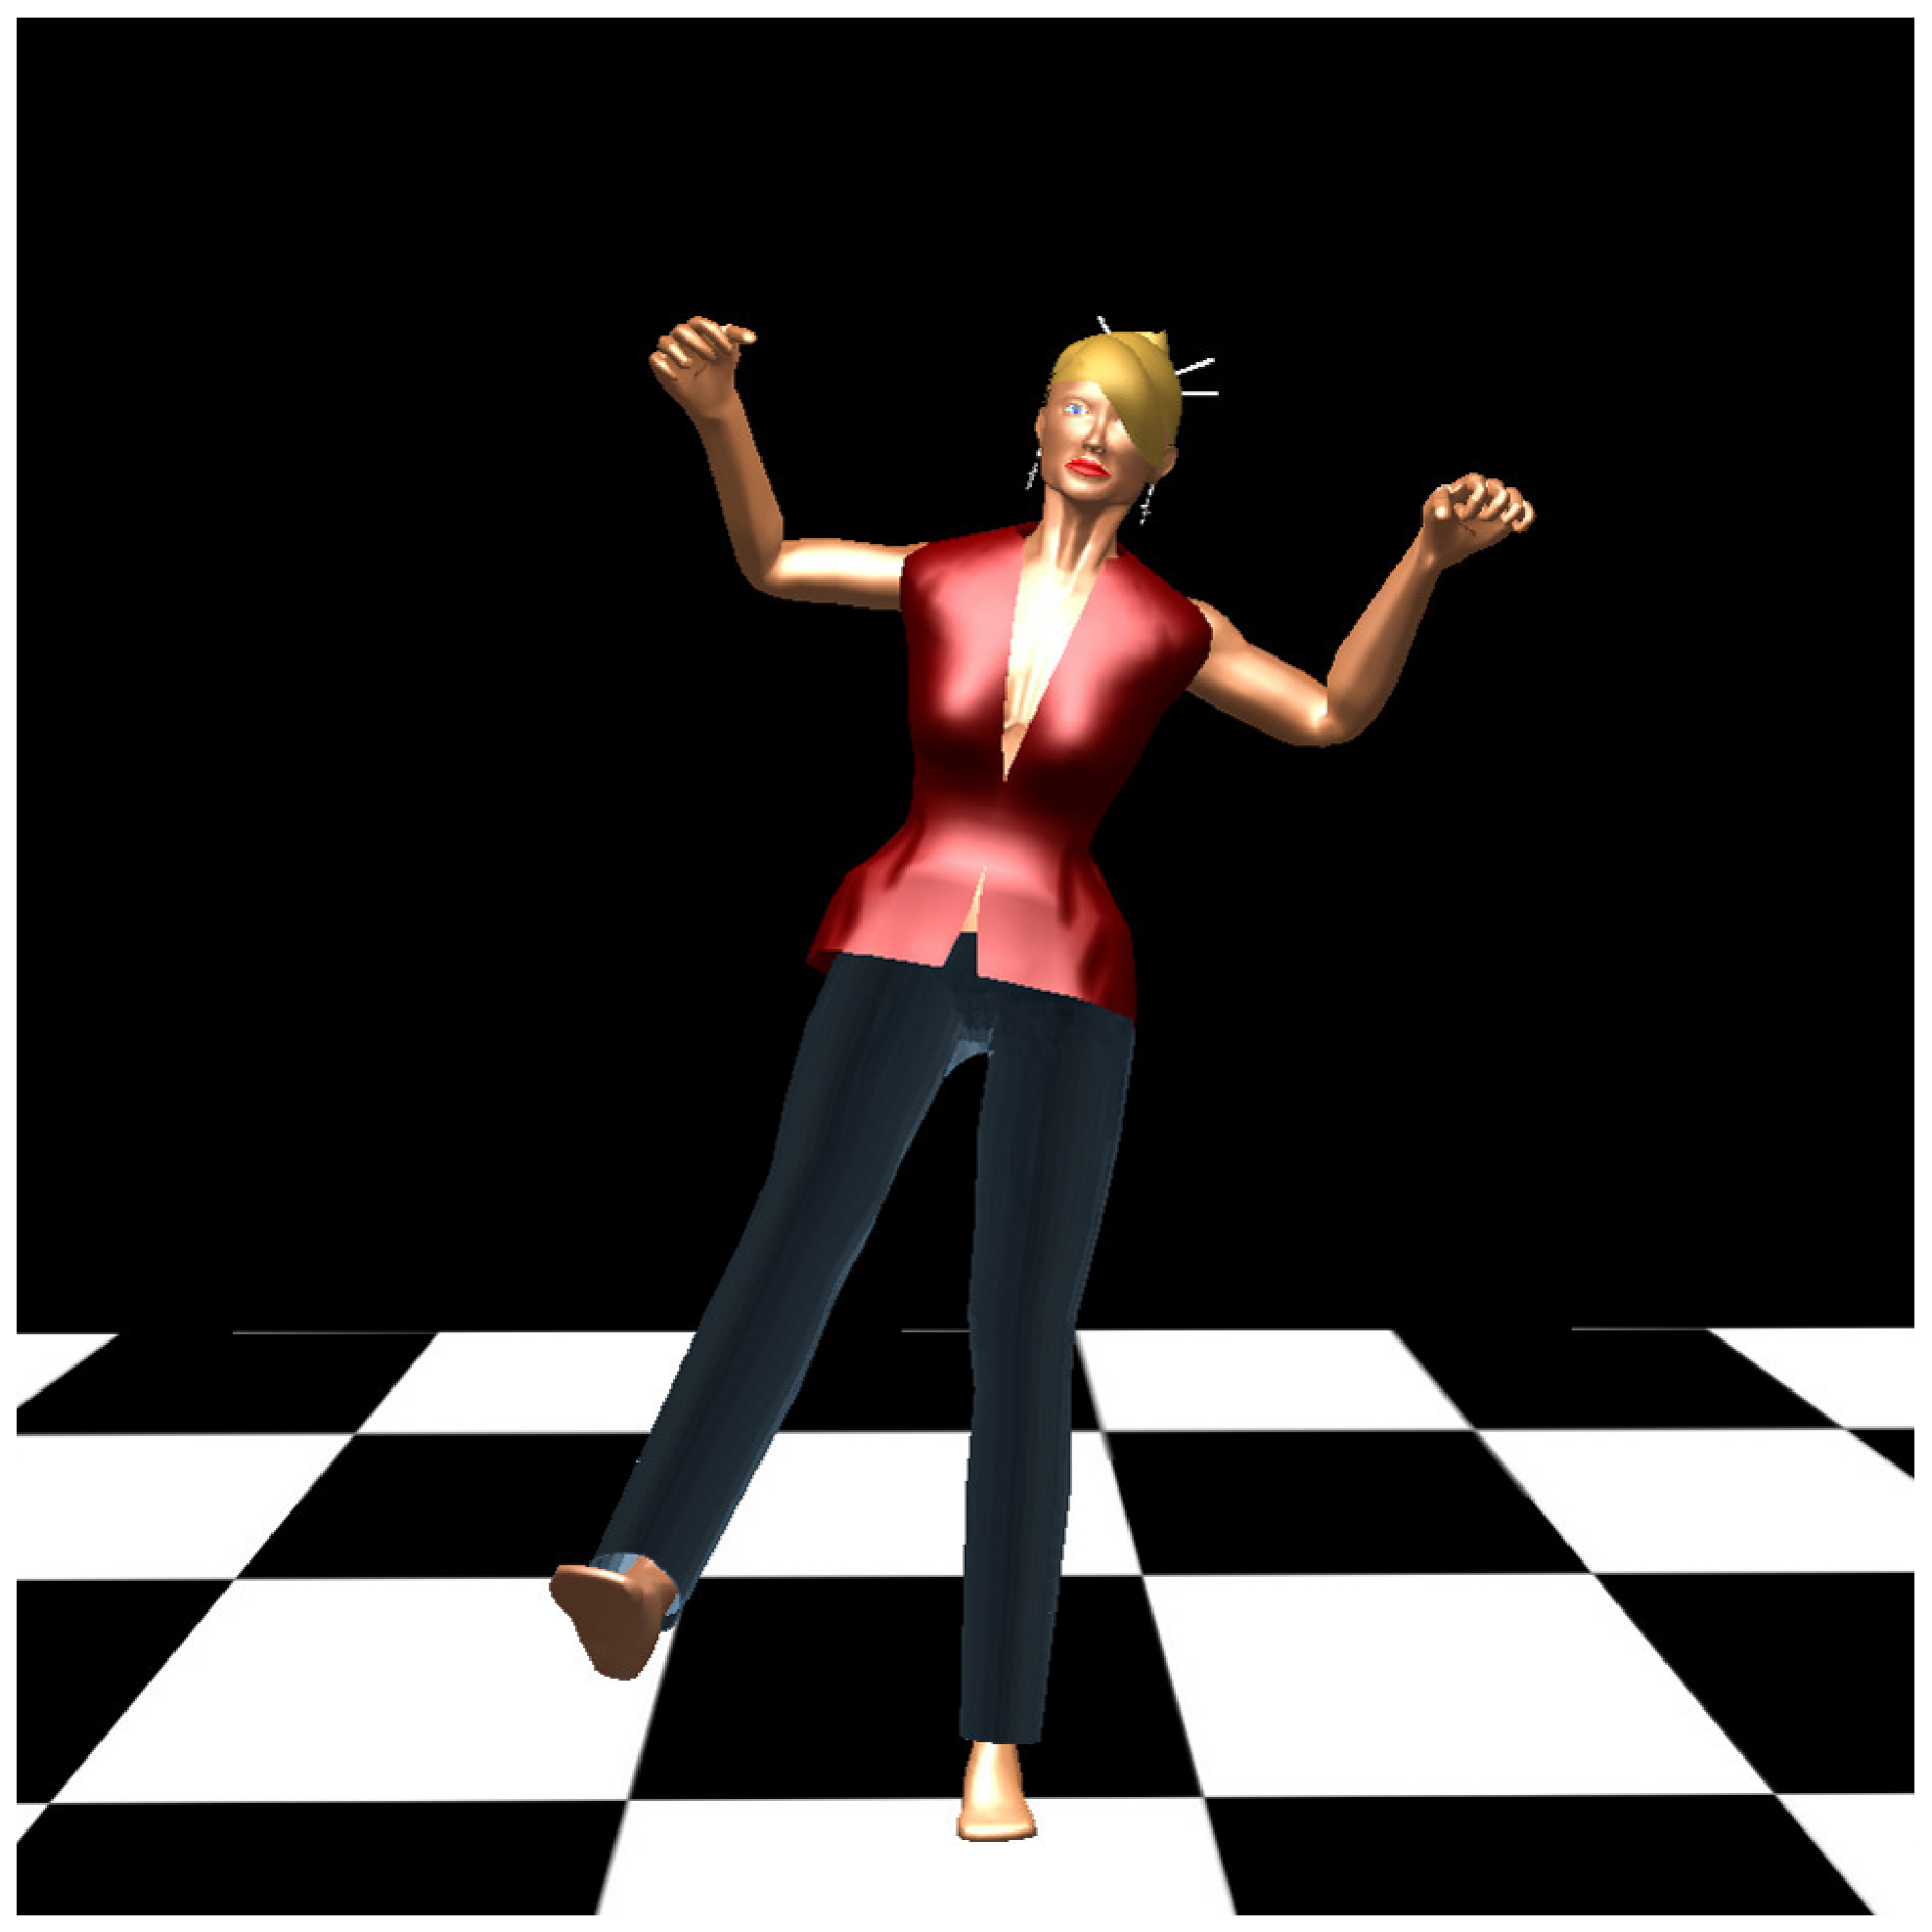
\includegraphics[width=0.250\textwidth]{./figures/jeans-1.eps}
	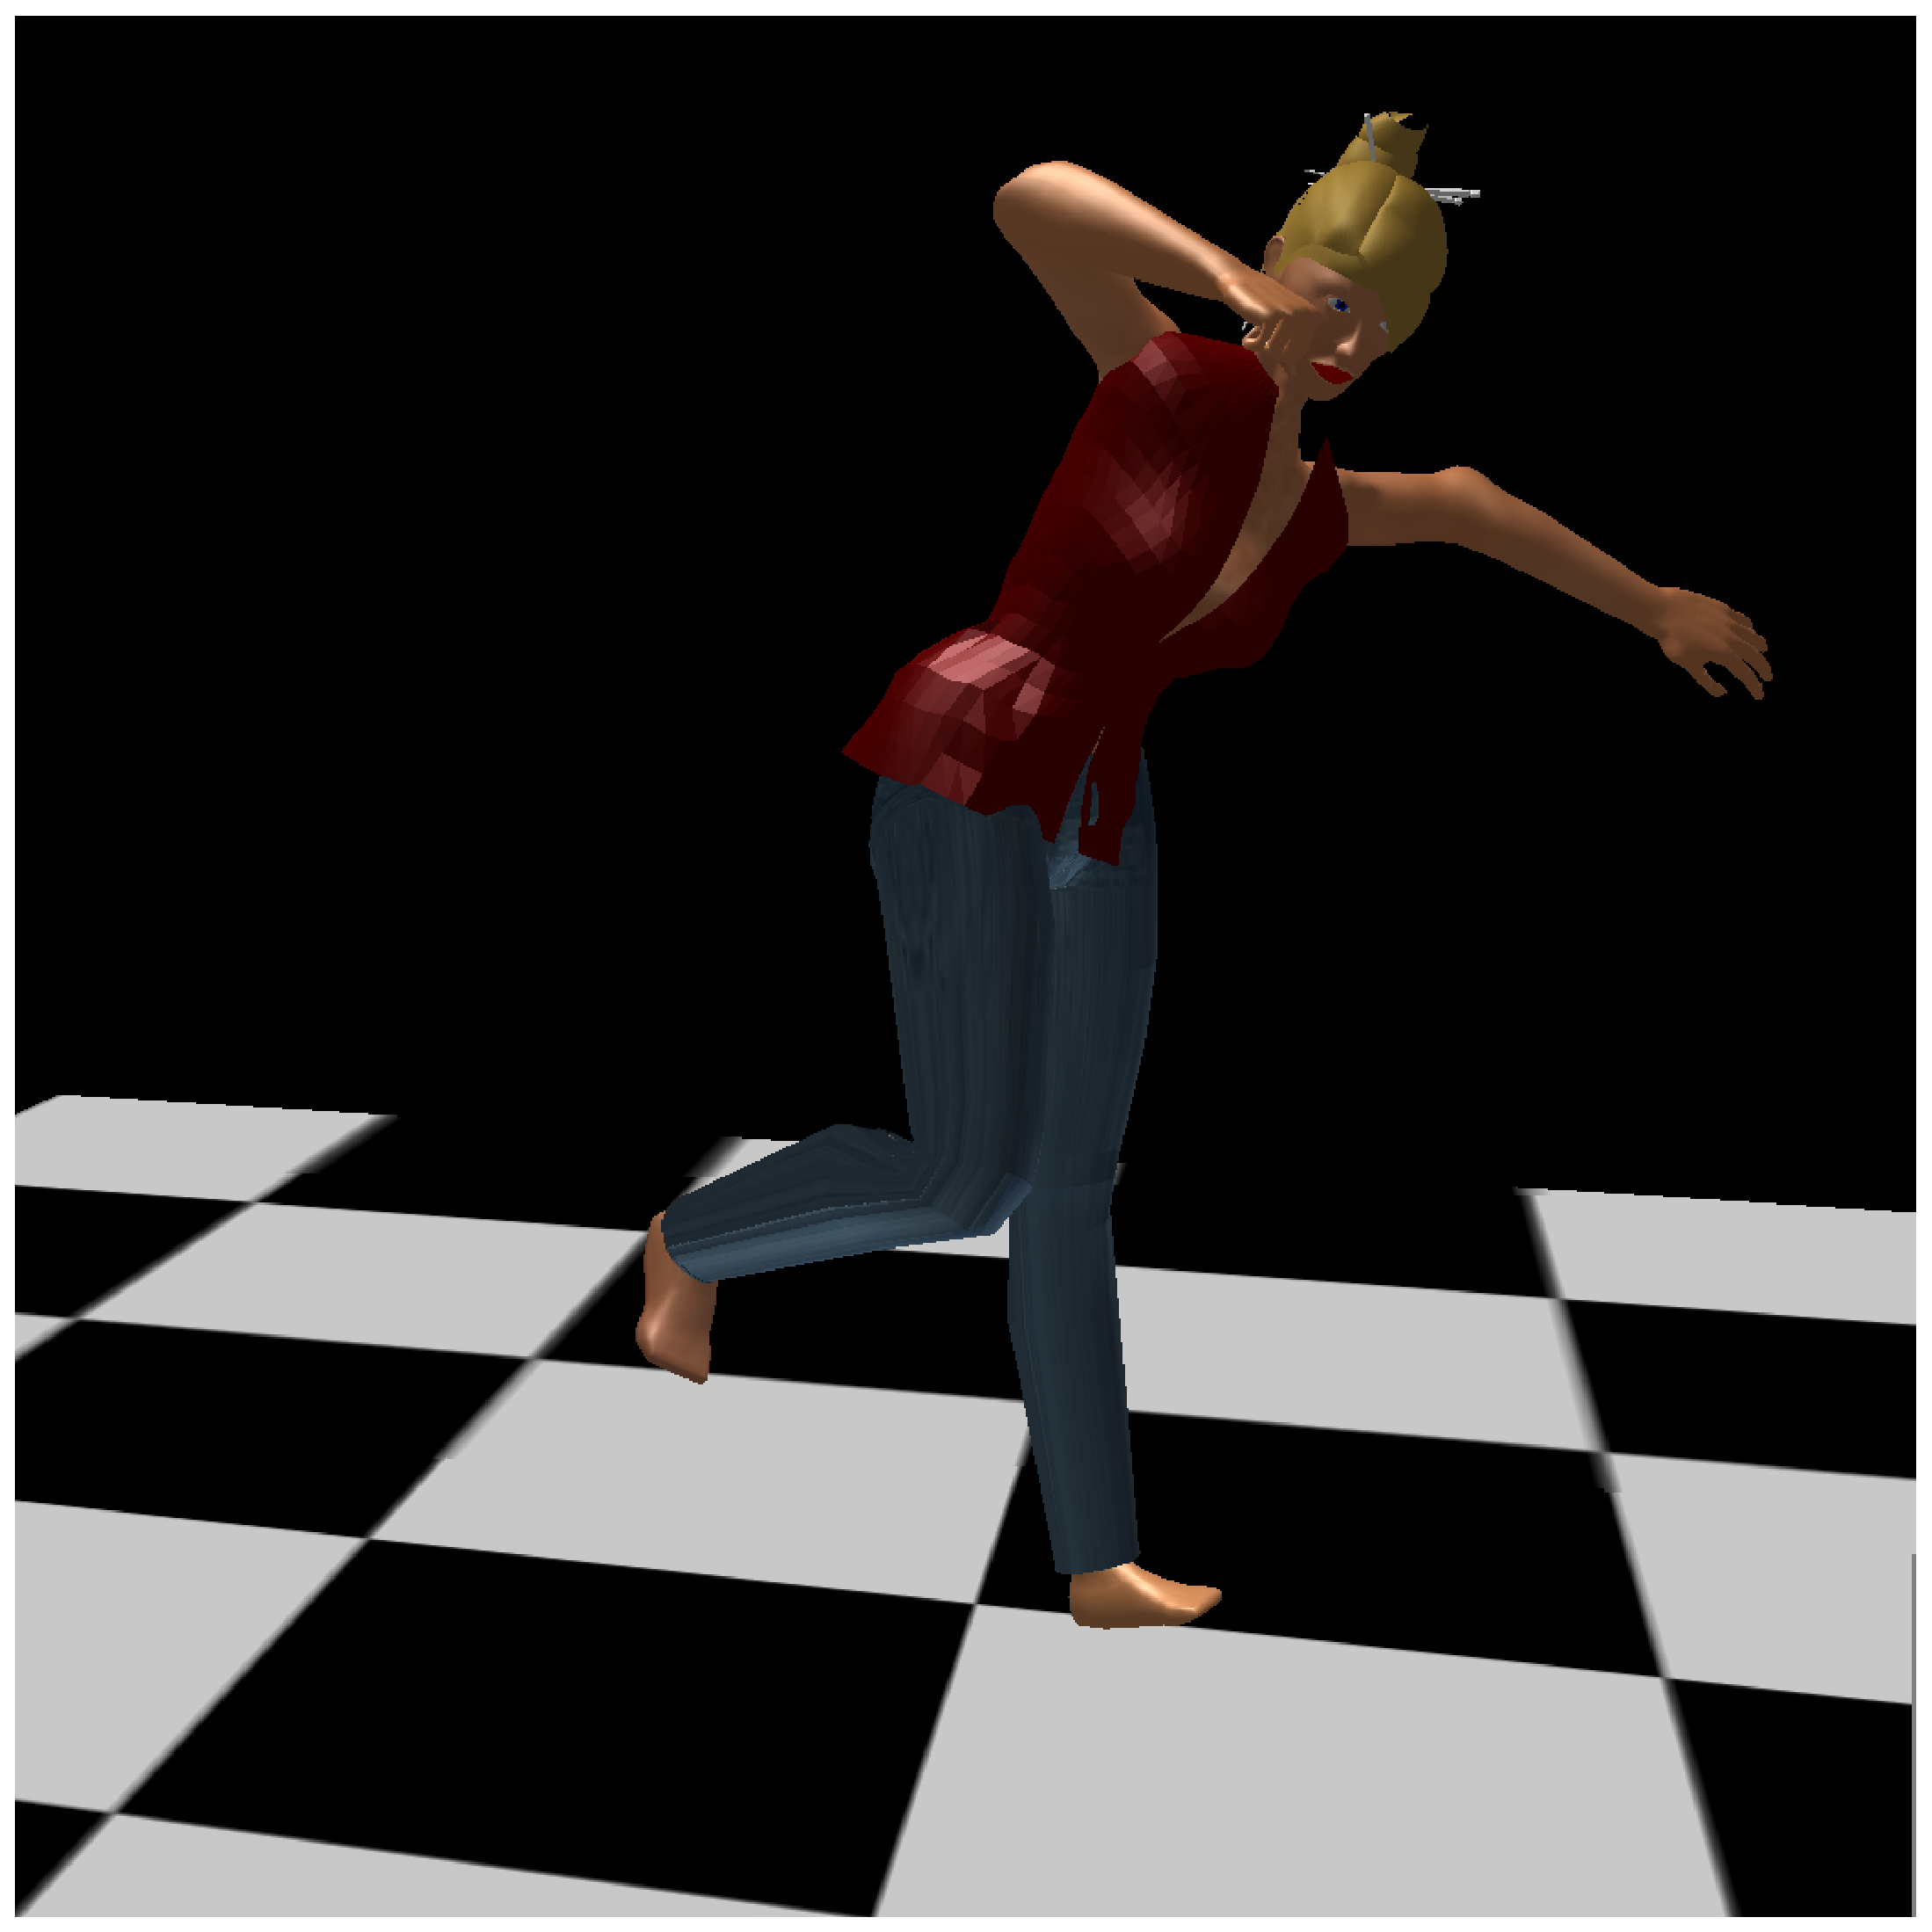
\includegraphics[width=0.250\textwidth]{./figures/jeans-2.eps}
	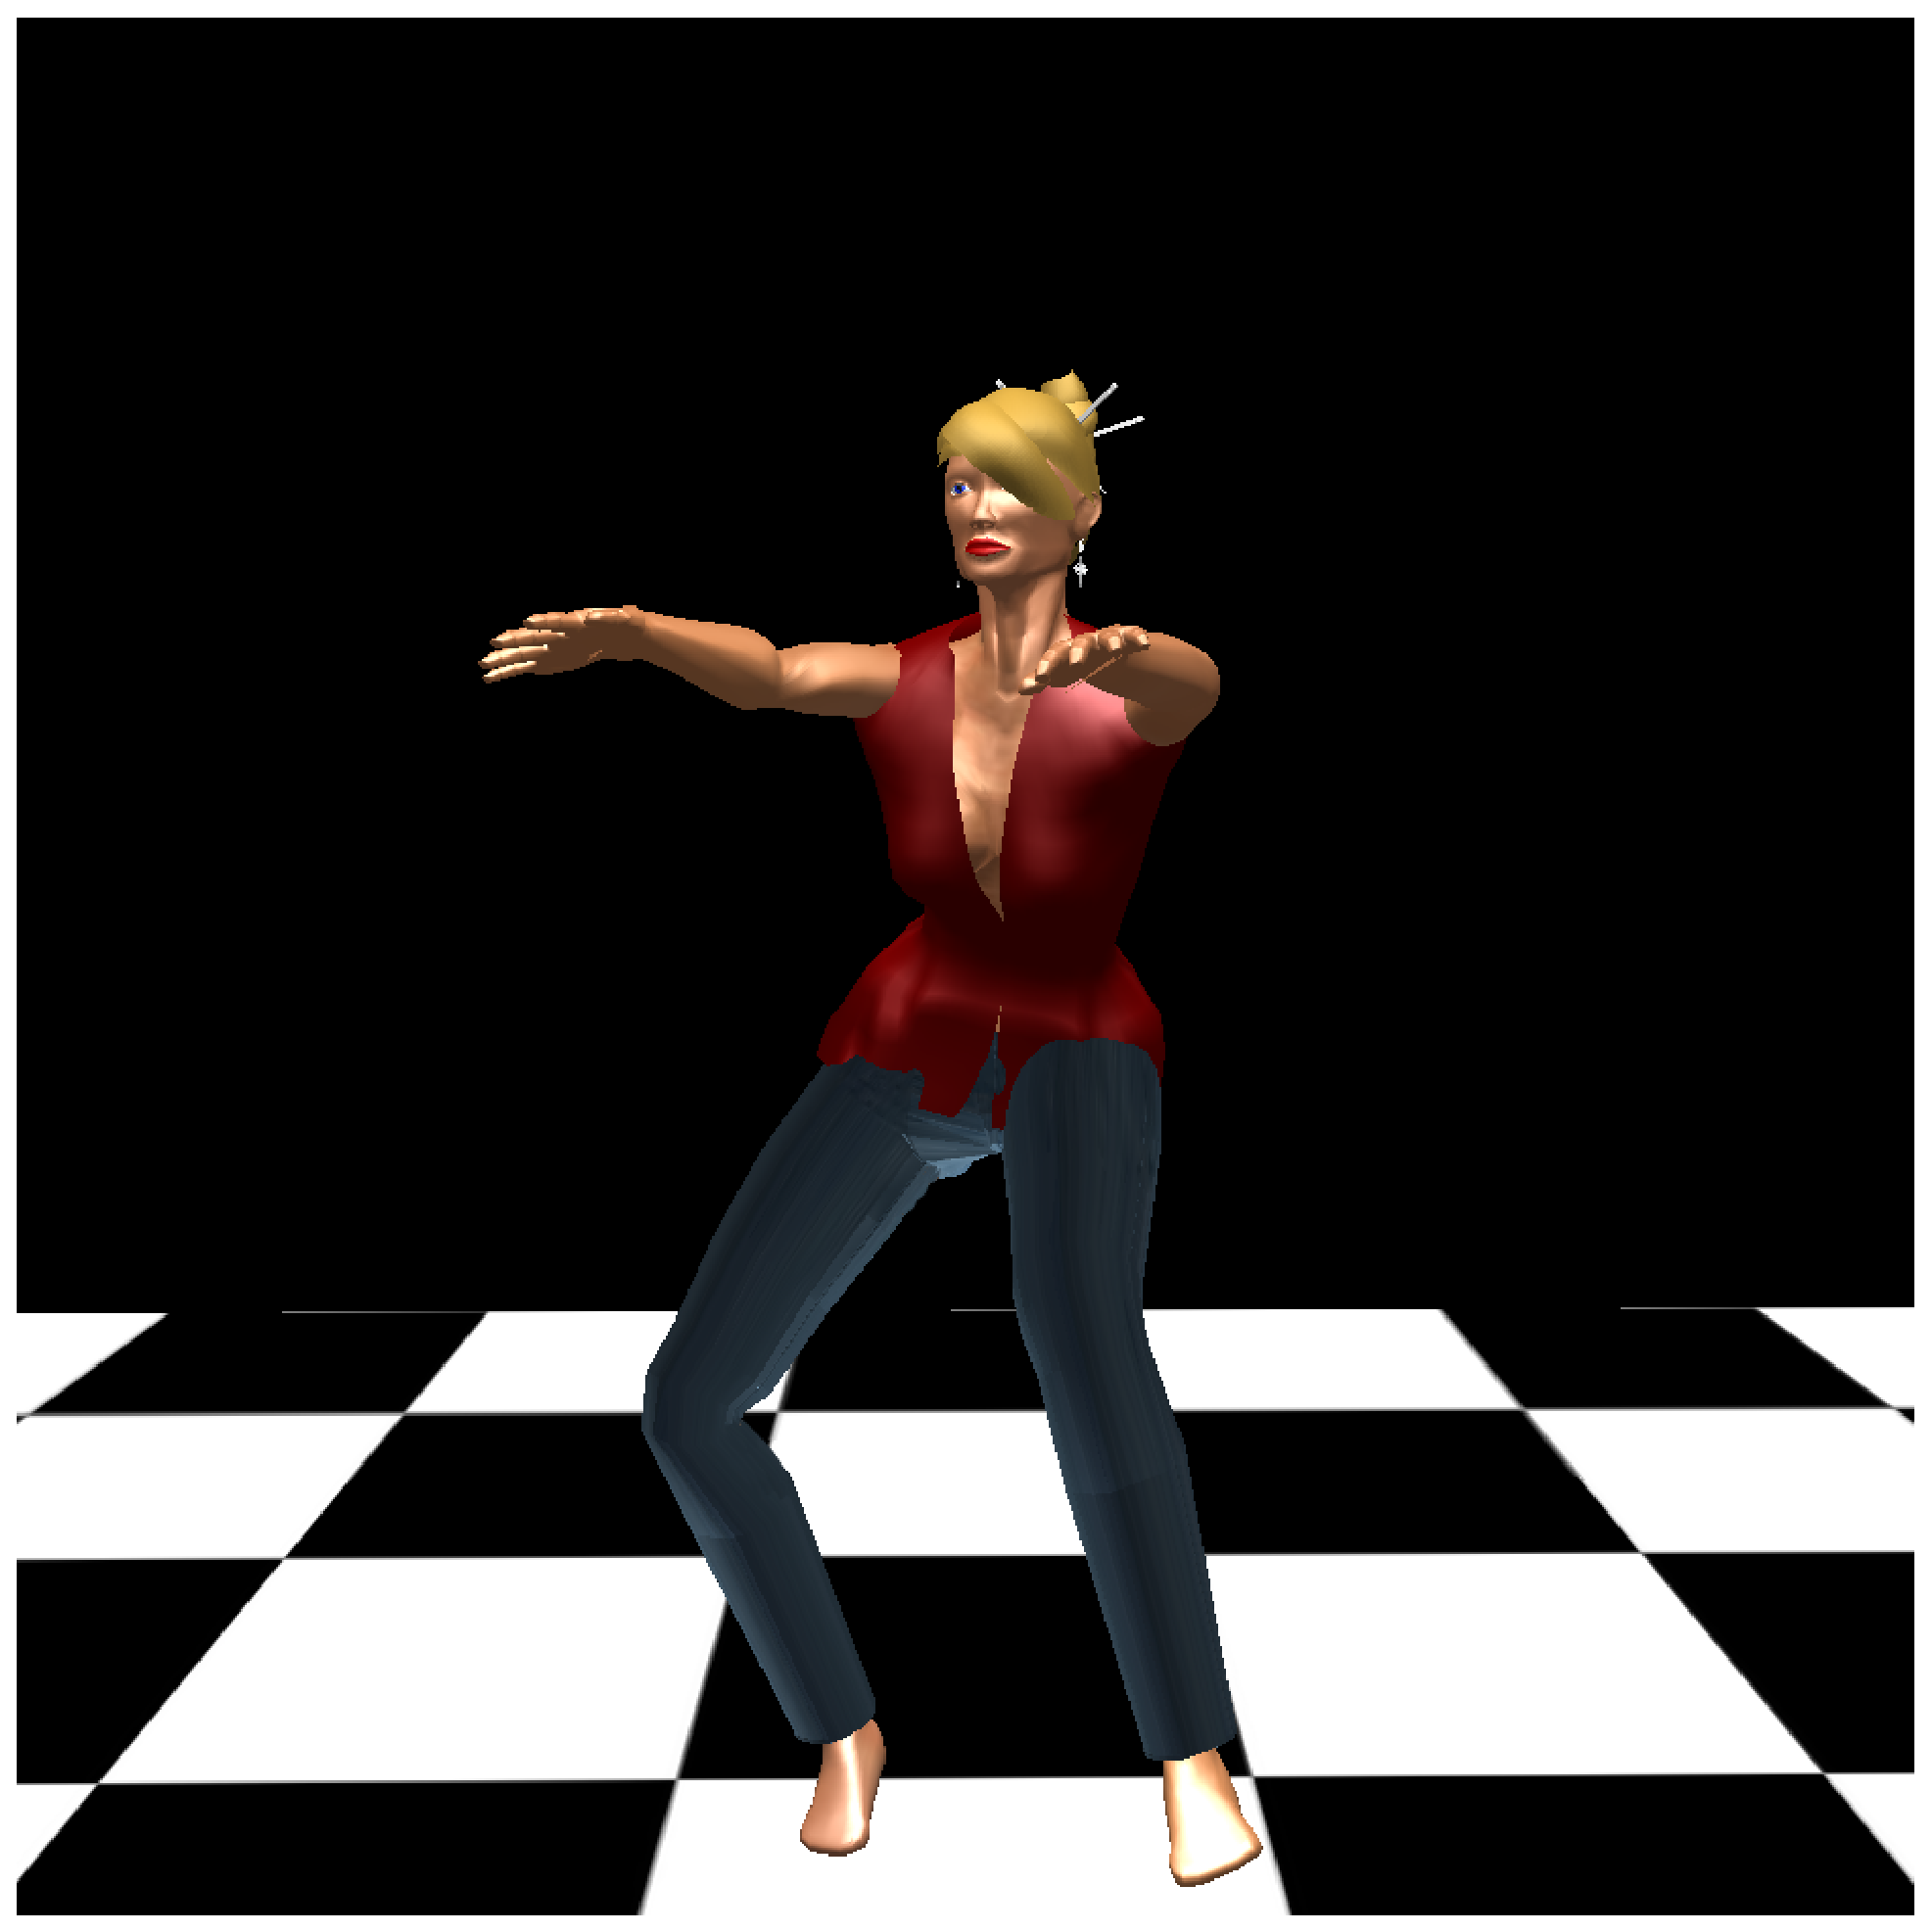
\includegraphics[width=0.250\textwidth]{./figures/jeans-3.eps}
	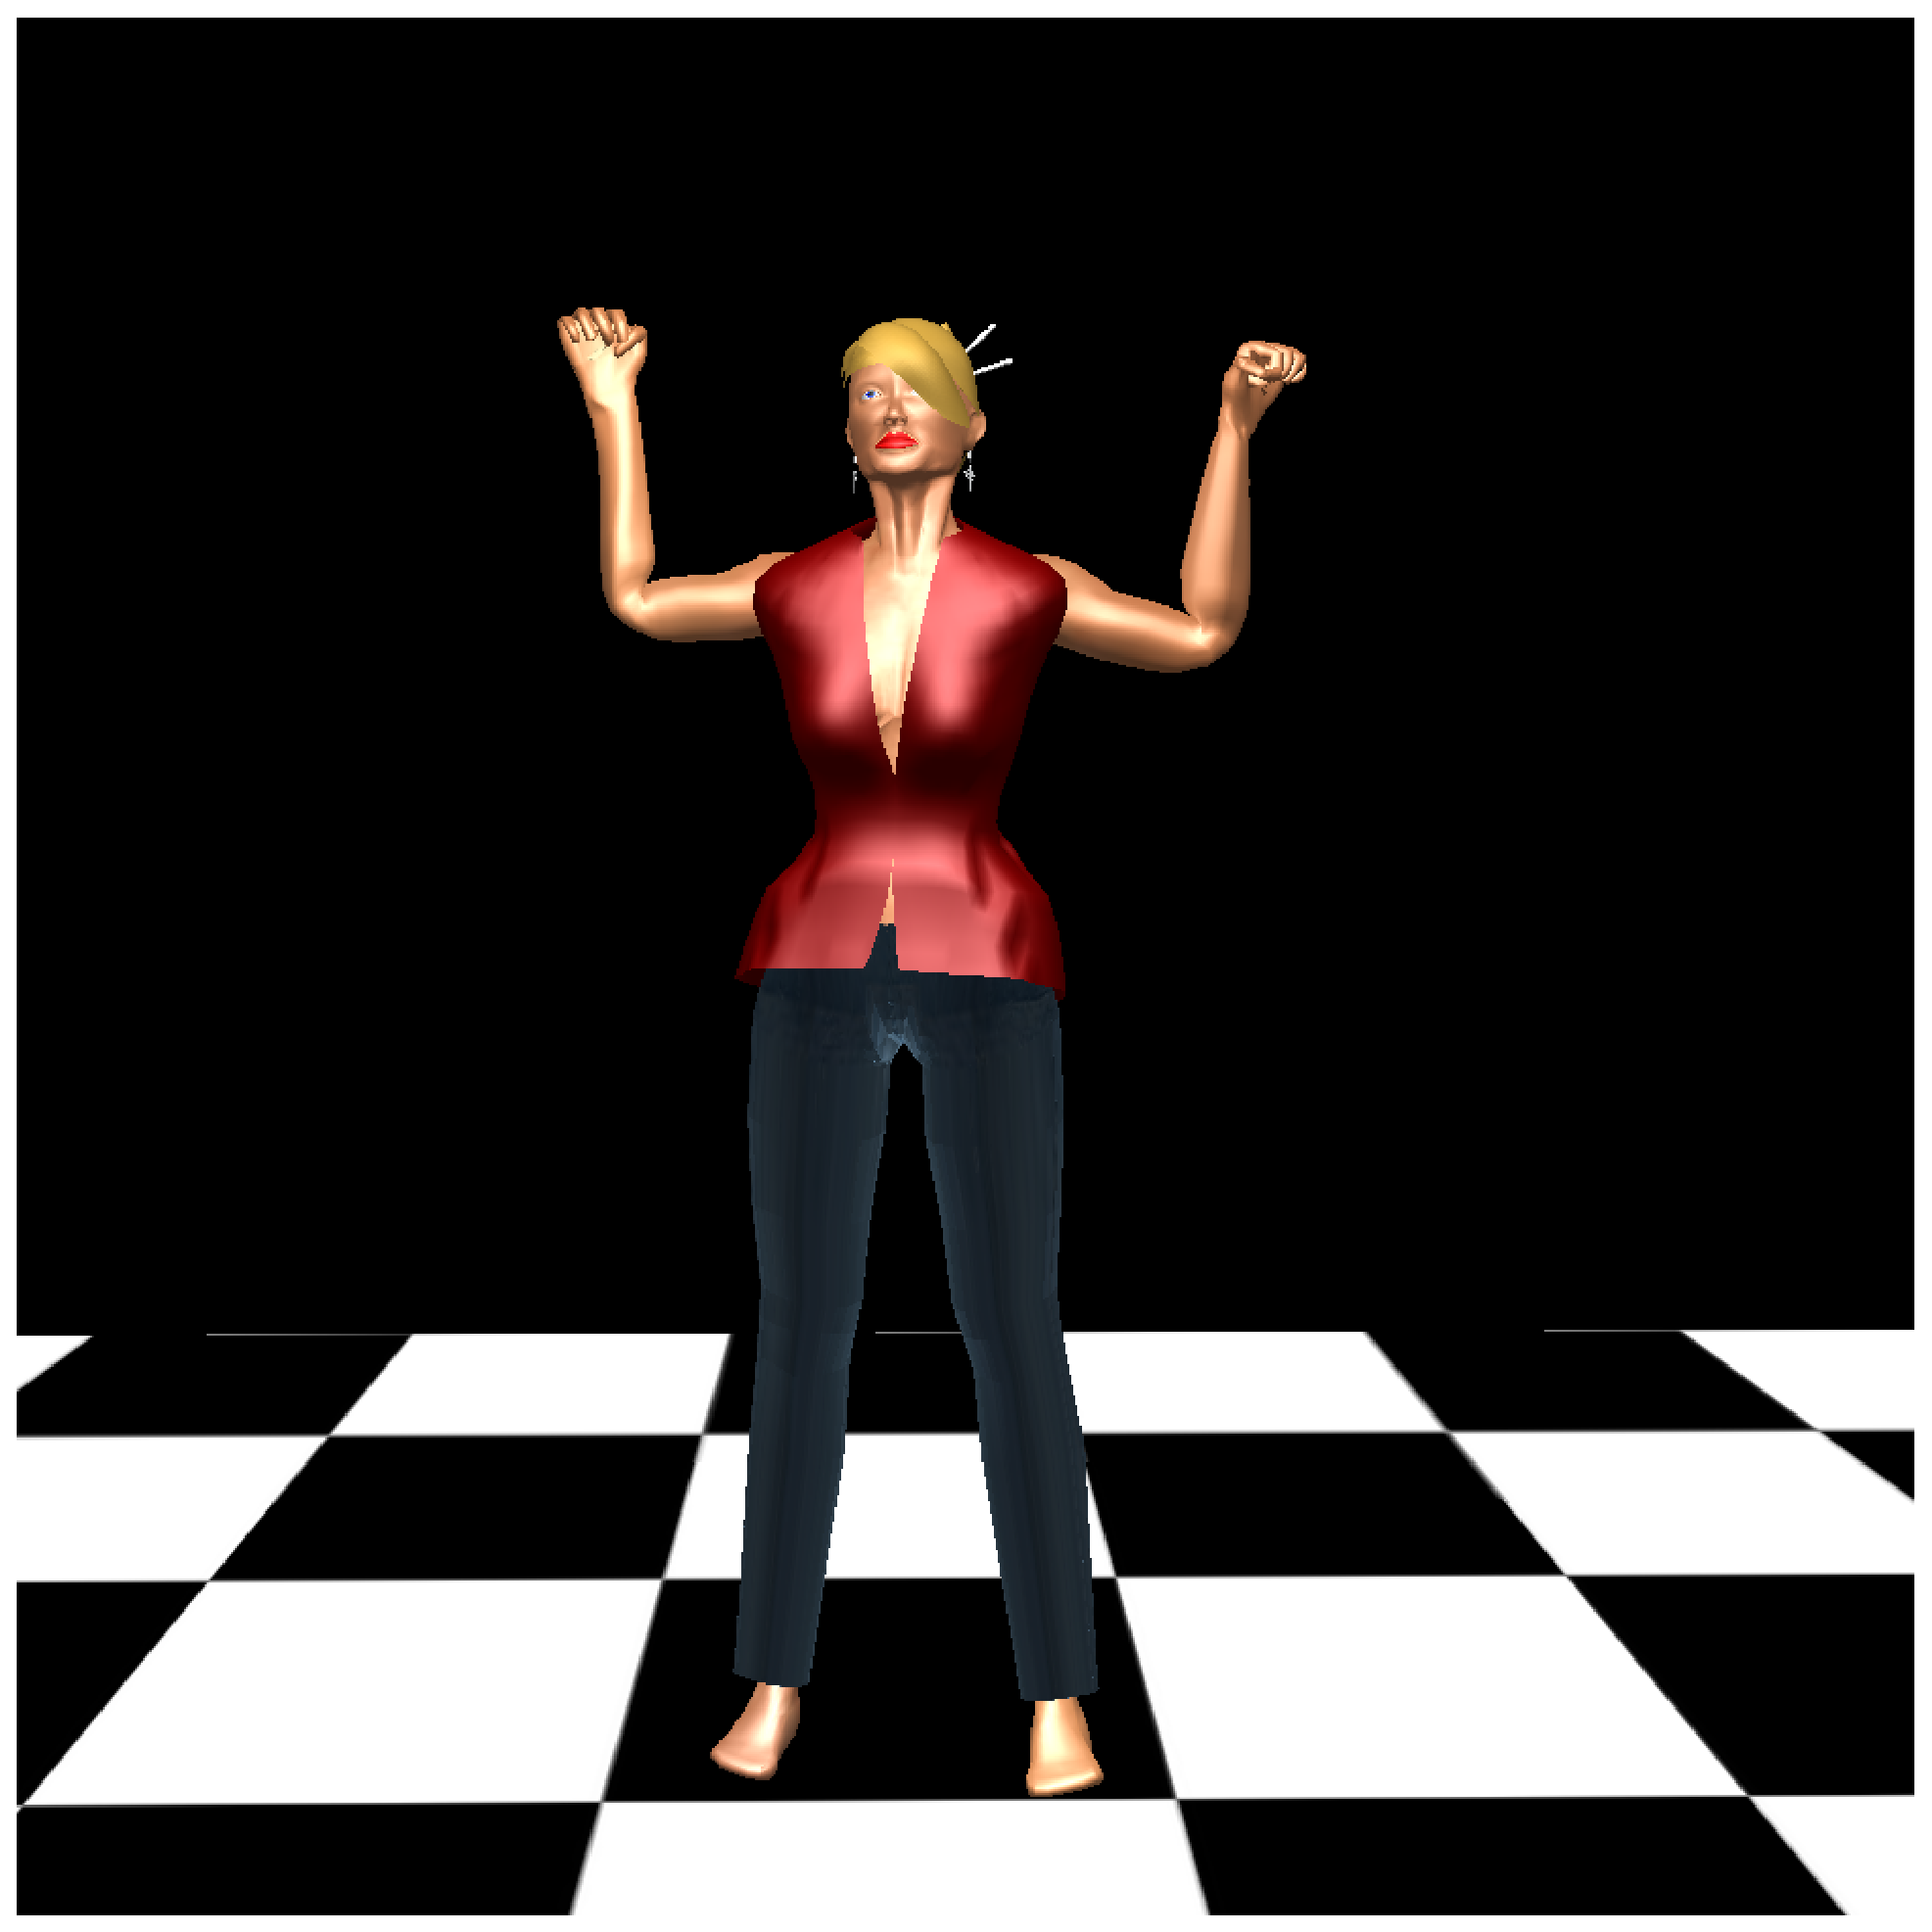
\includegraphics[width=0.250\textwidth]{./figures/jeans-4.eps}
	}
	\centerline{(b)}
	\centerline{\ }
	\centerline{
	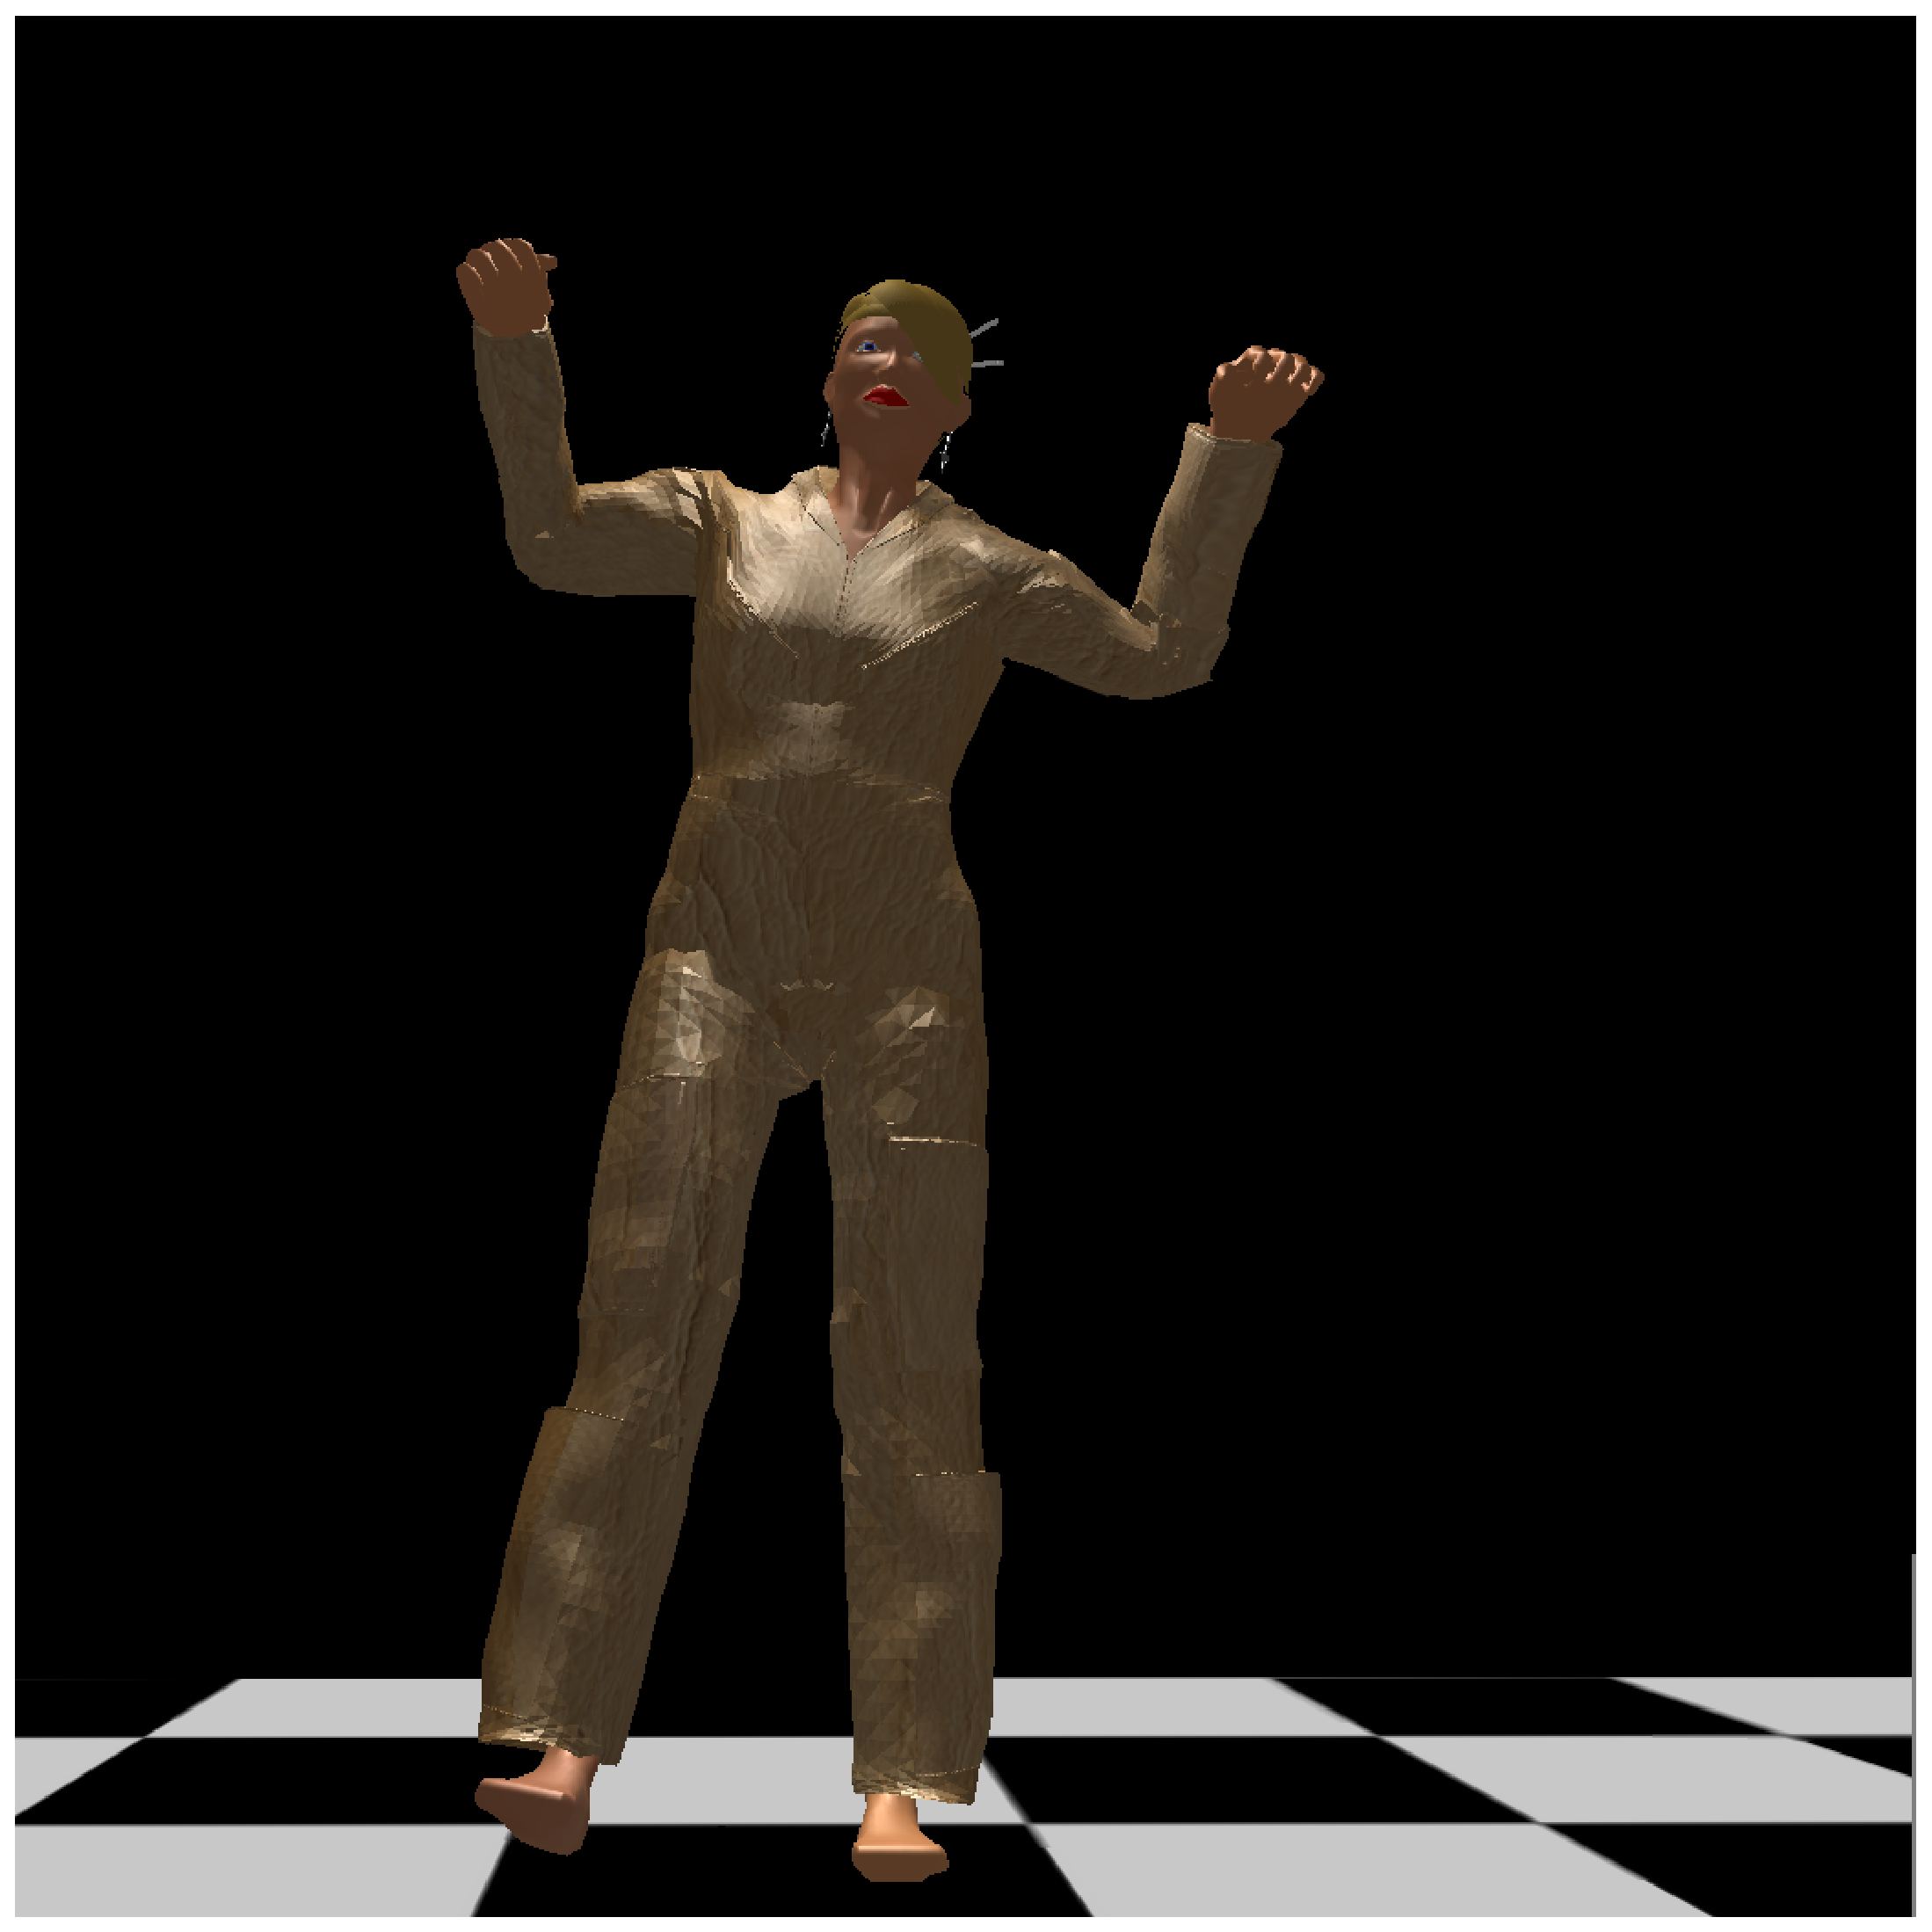
\includegraphics[width=0.250\textwidth]{./figures/flightsuit-1.eps}
	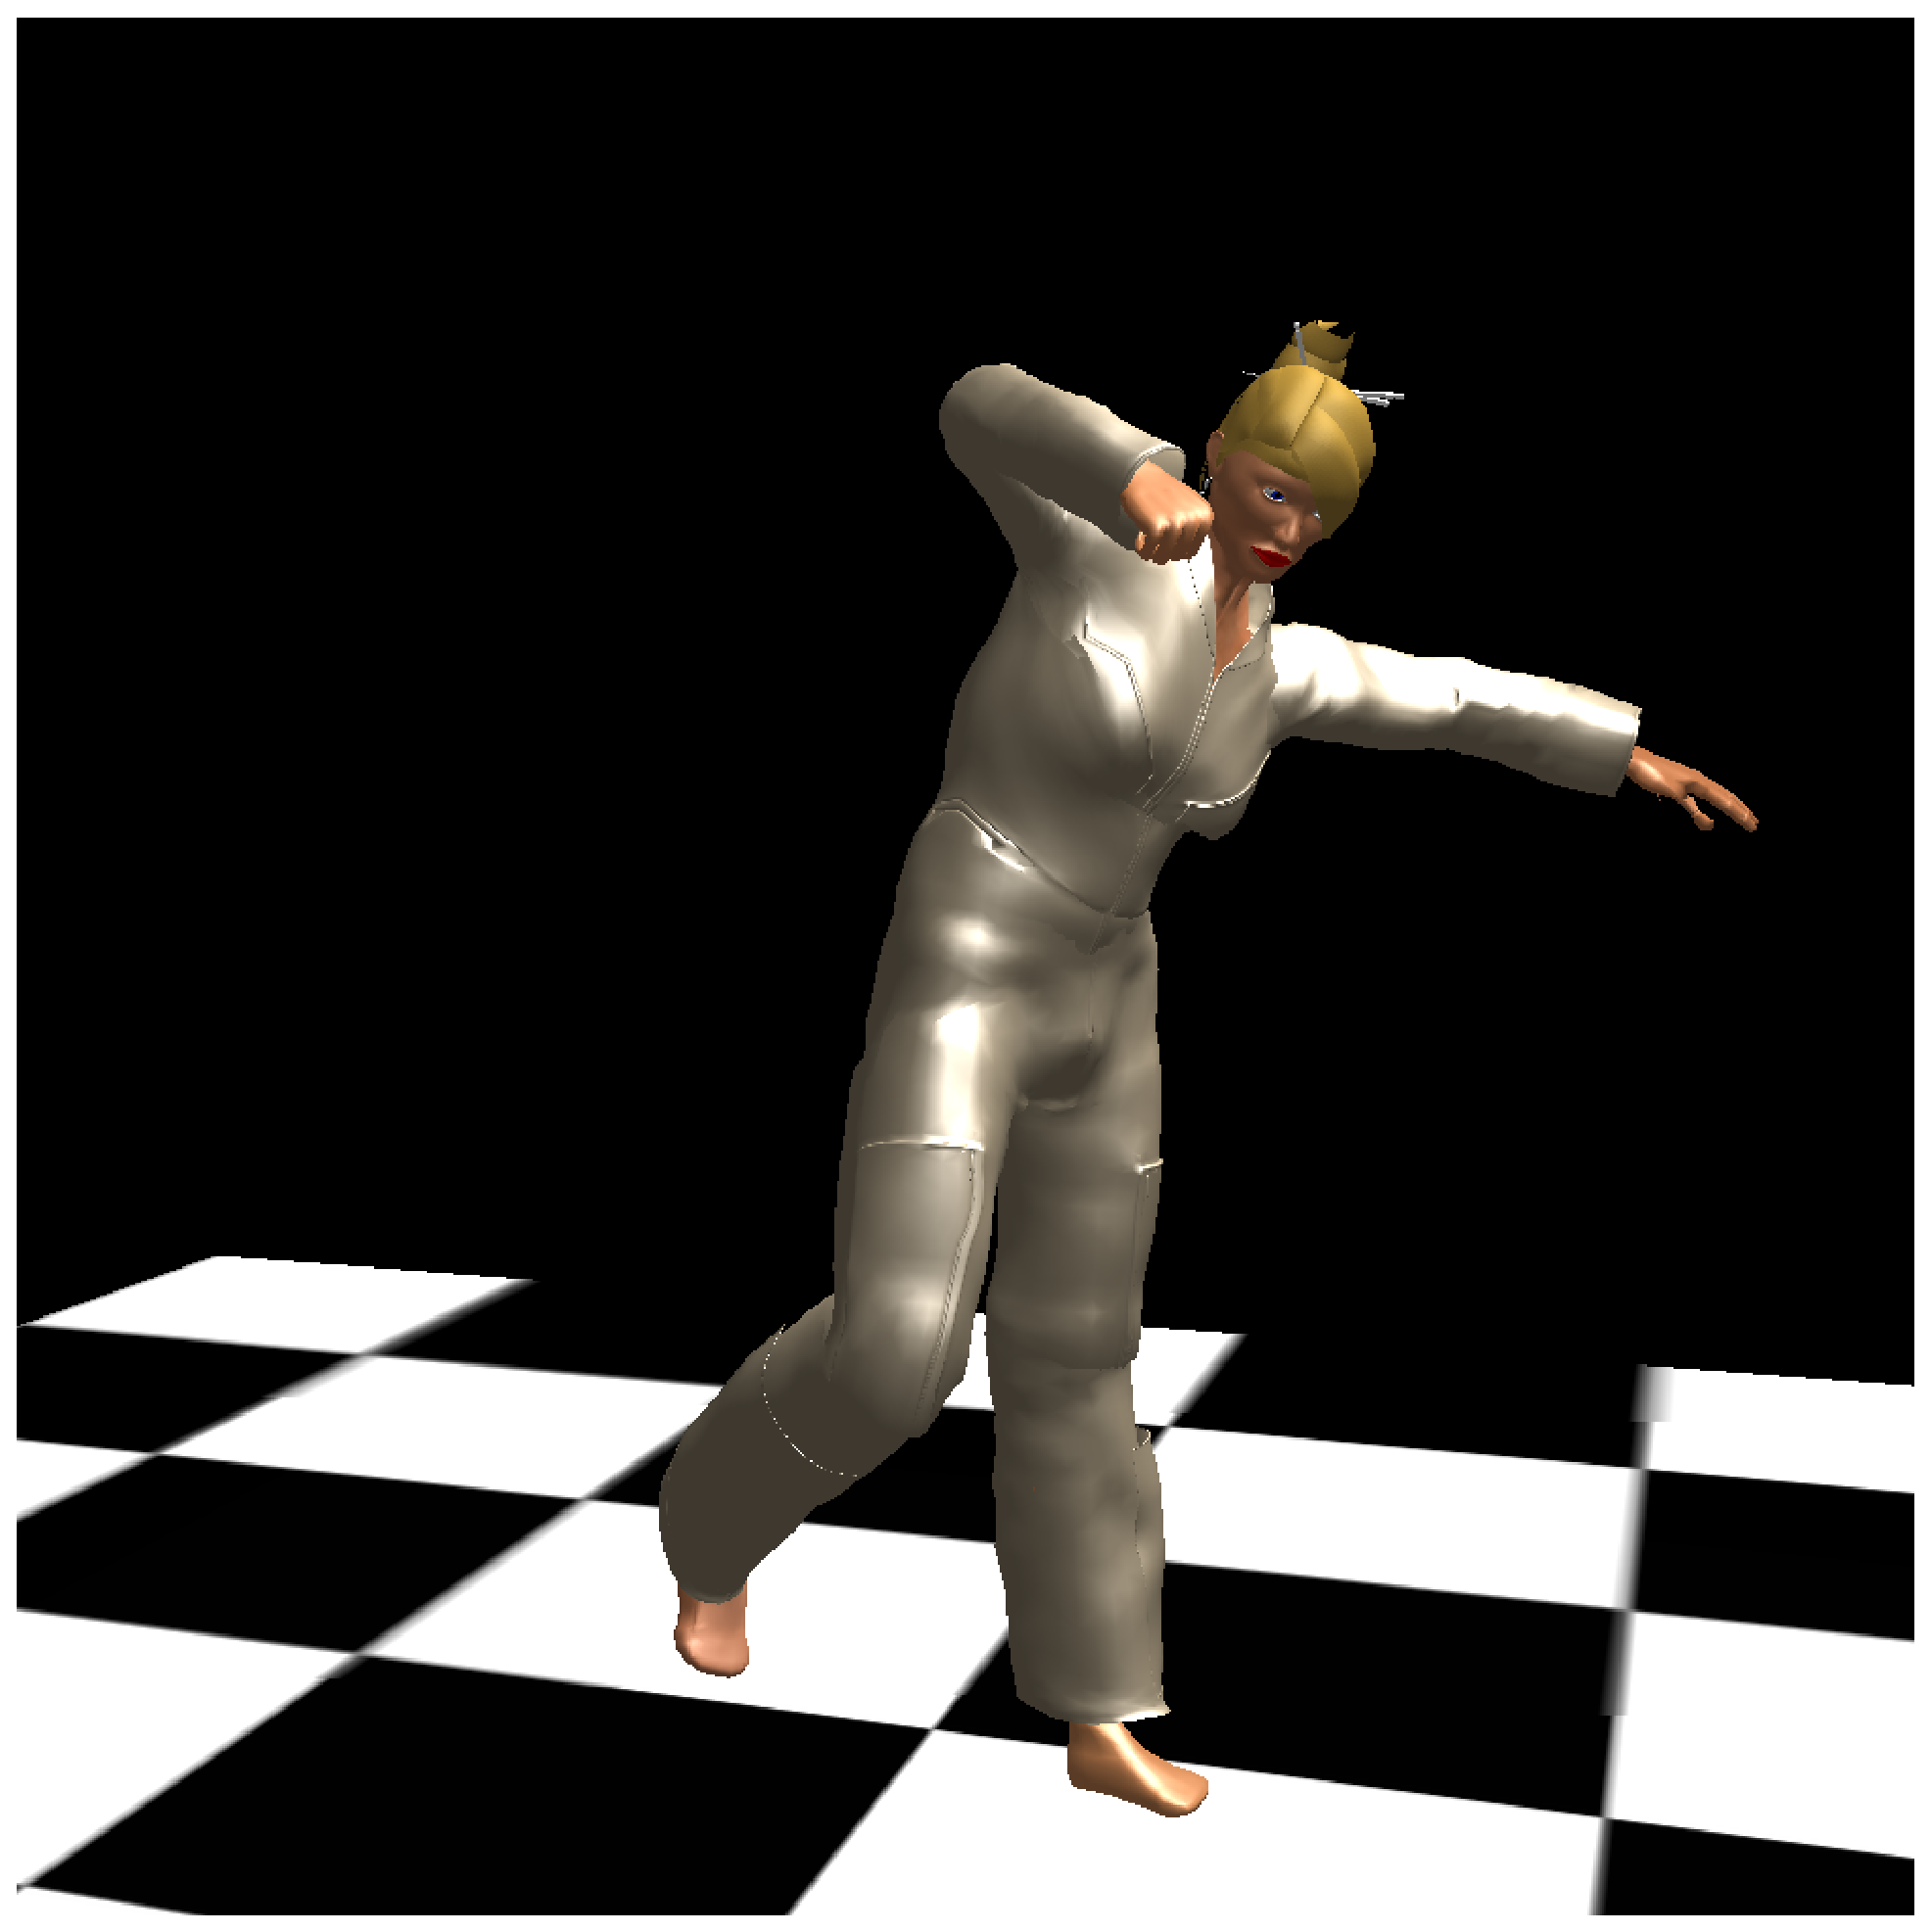
\includegraphics[width=0.250\textwidth]{./figures/flightsuit-2.eps}
	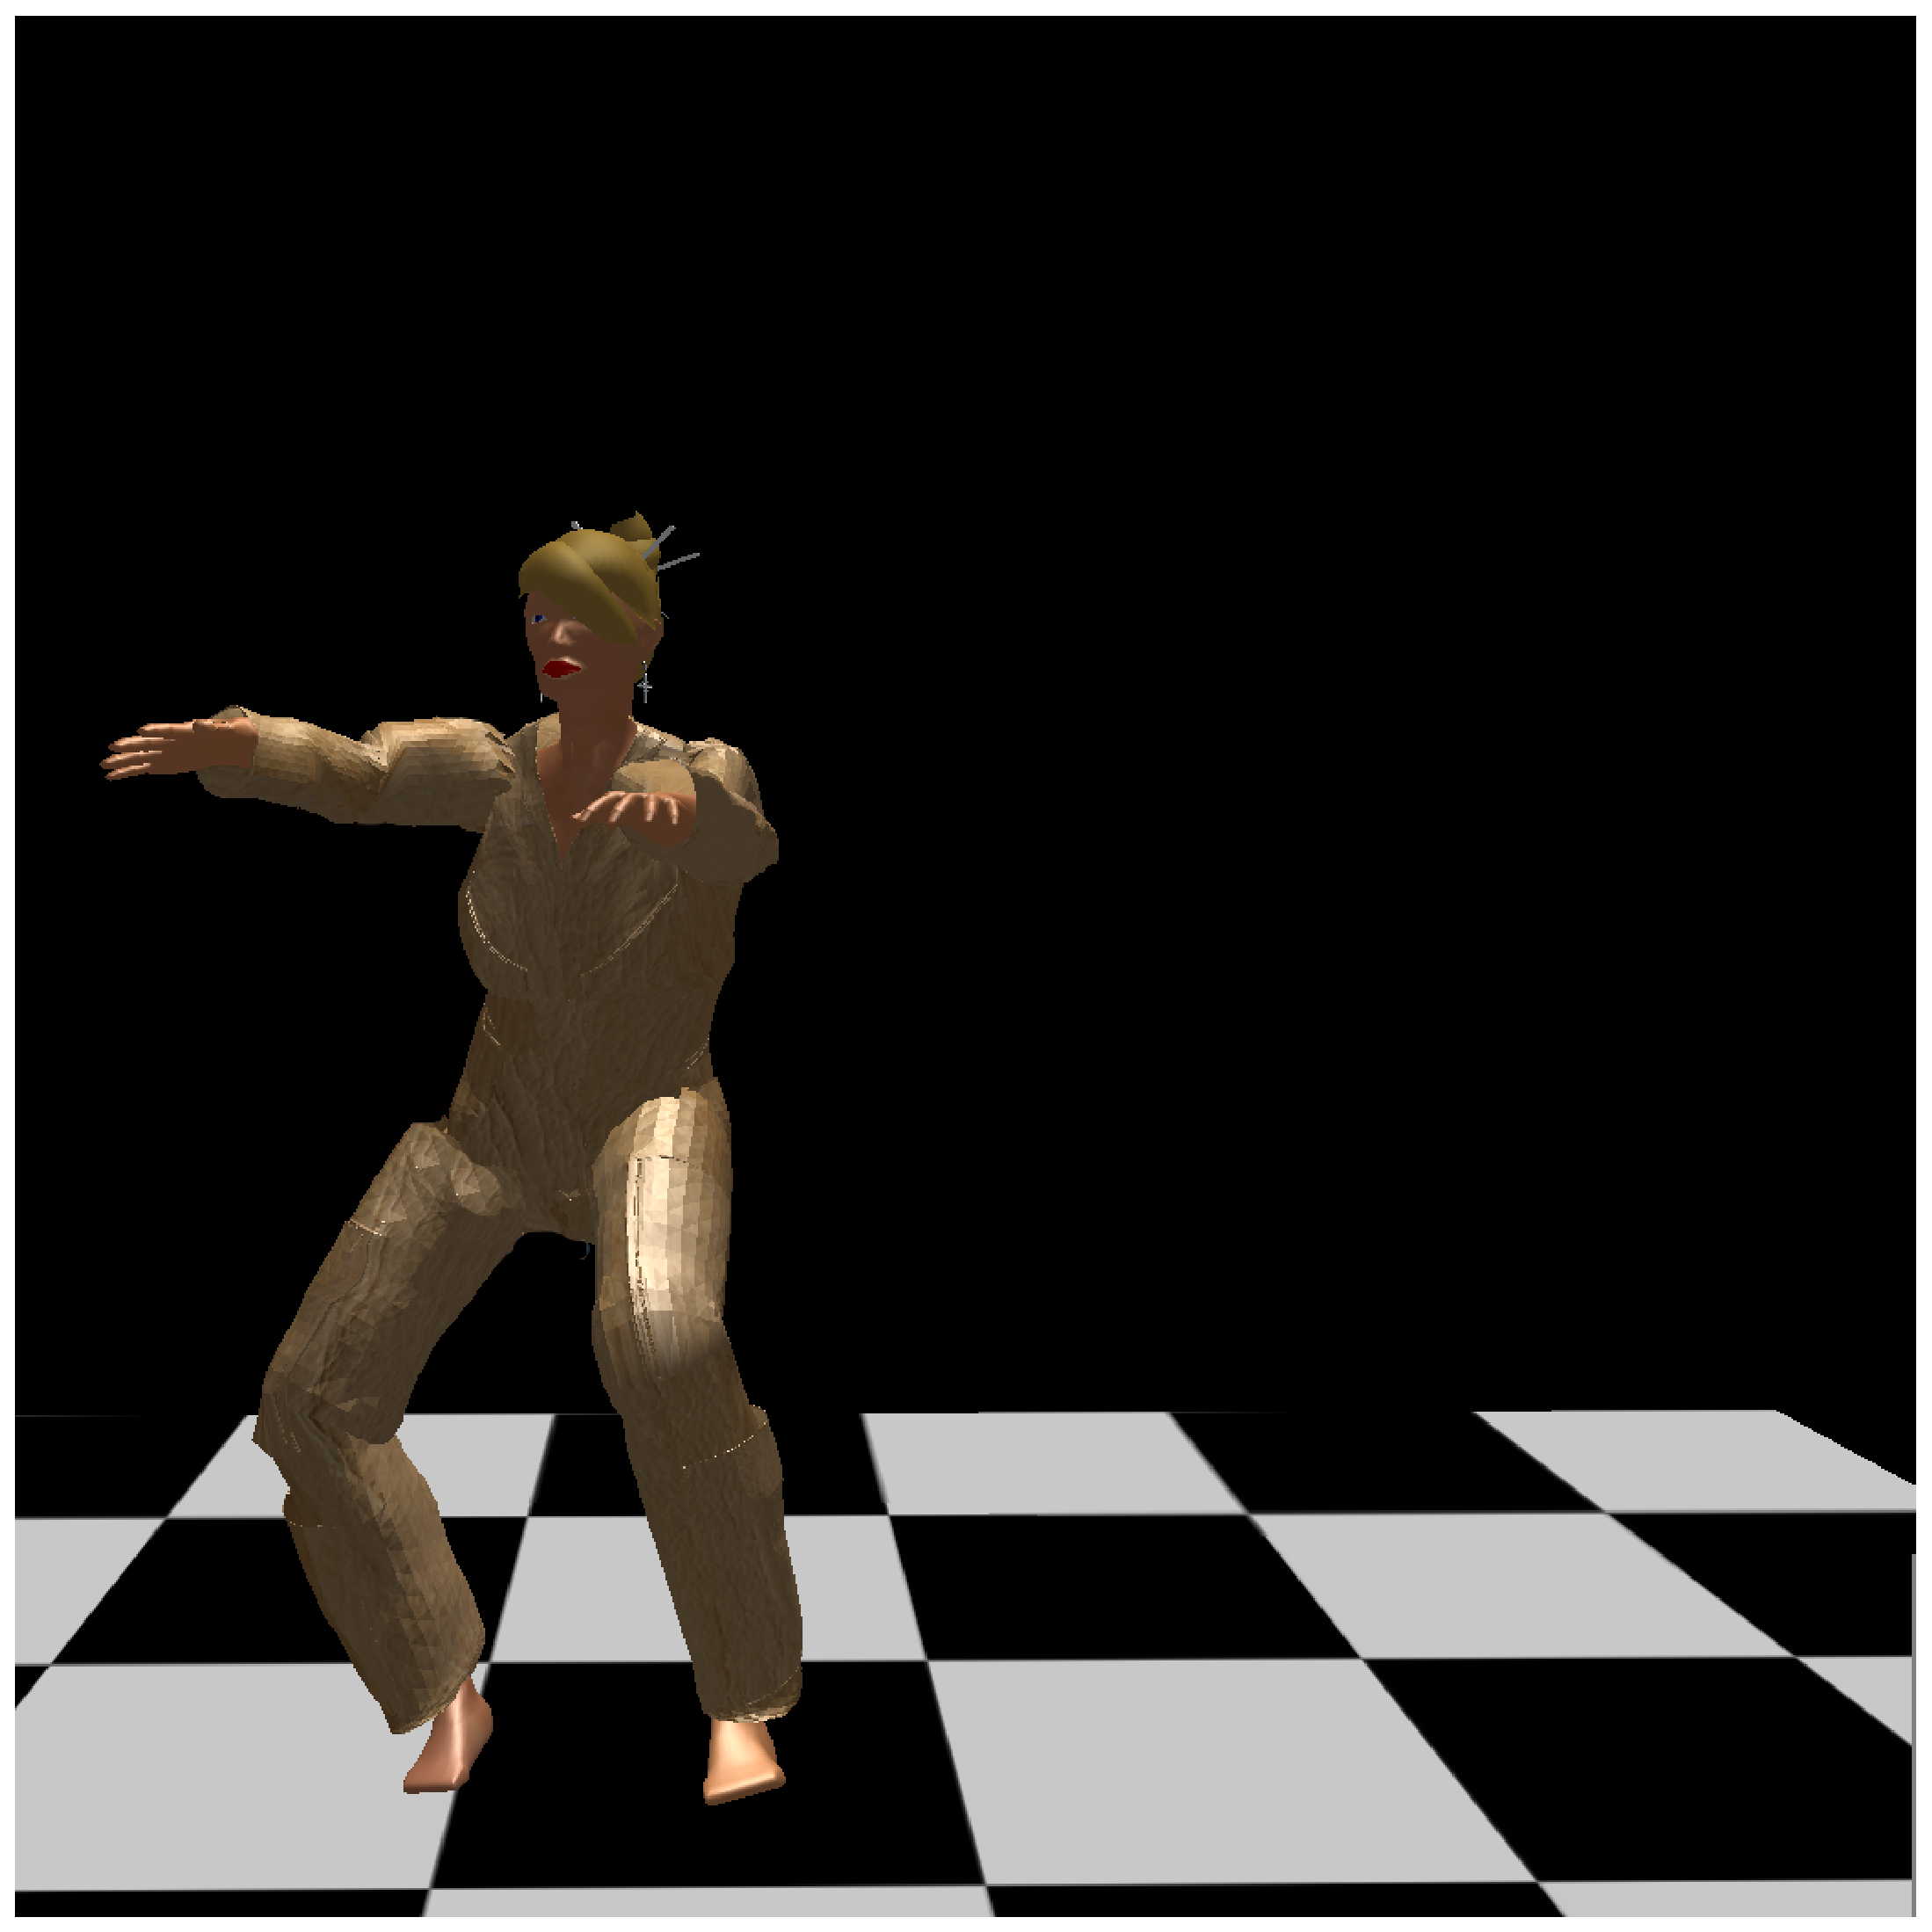
\includegraphics[width=0.250\textwidth]{./figures/flightsuit-3.eps}
	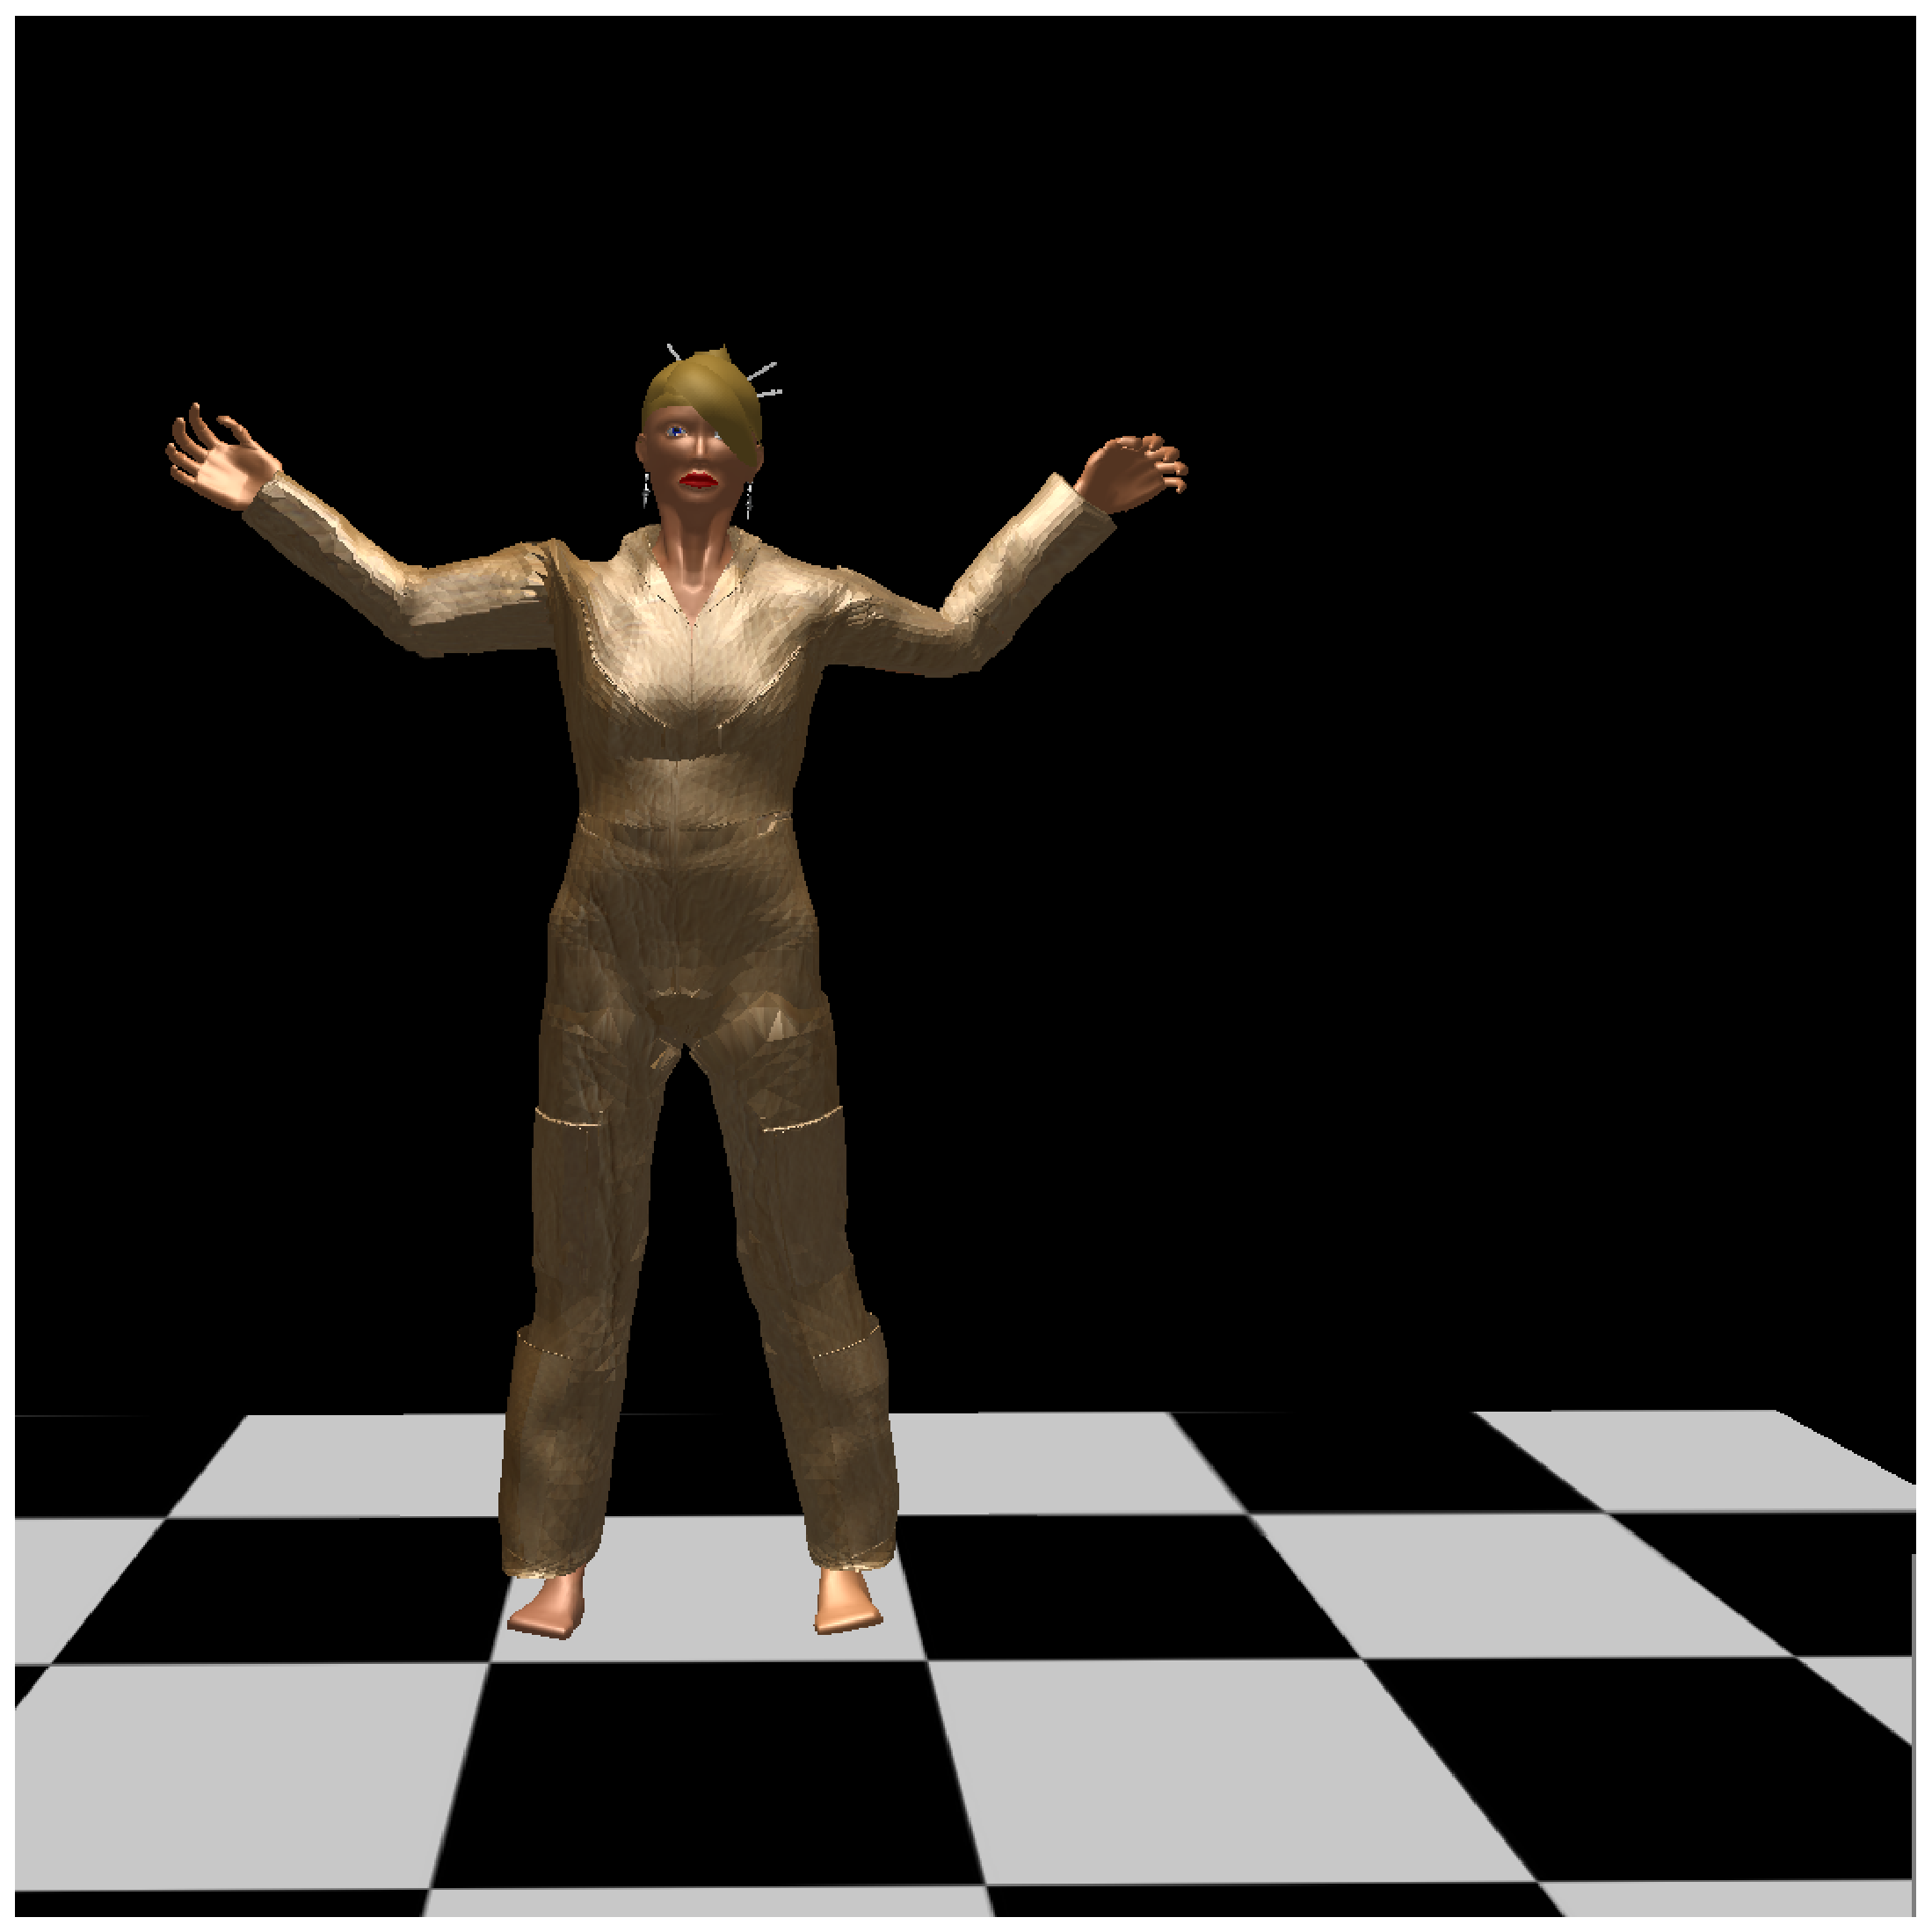
\includegraphics[width=0.250\textwidth]{./figures/flightsuit-4.eps}
	}
	\centerline{(c)}
	\caption{Examples of different garments on a model with different postures: (a) sun dress, (b) jeans and vest, and 
	(c) flight suit.}
	\label{fig:examples}
\end{figure}

\begin{figure}[htbp] 
	\centerline{
	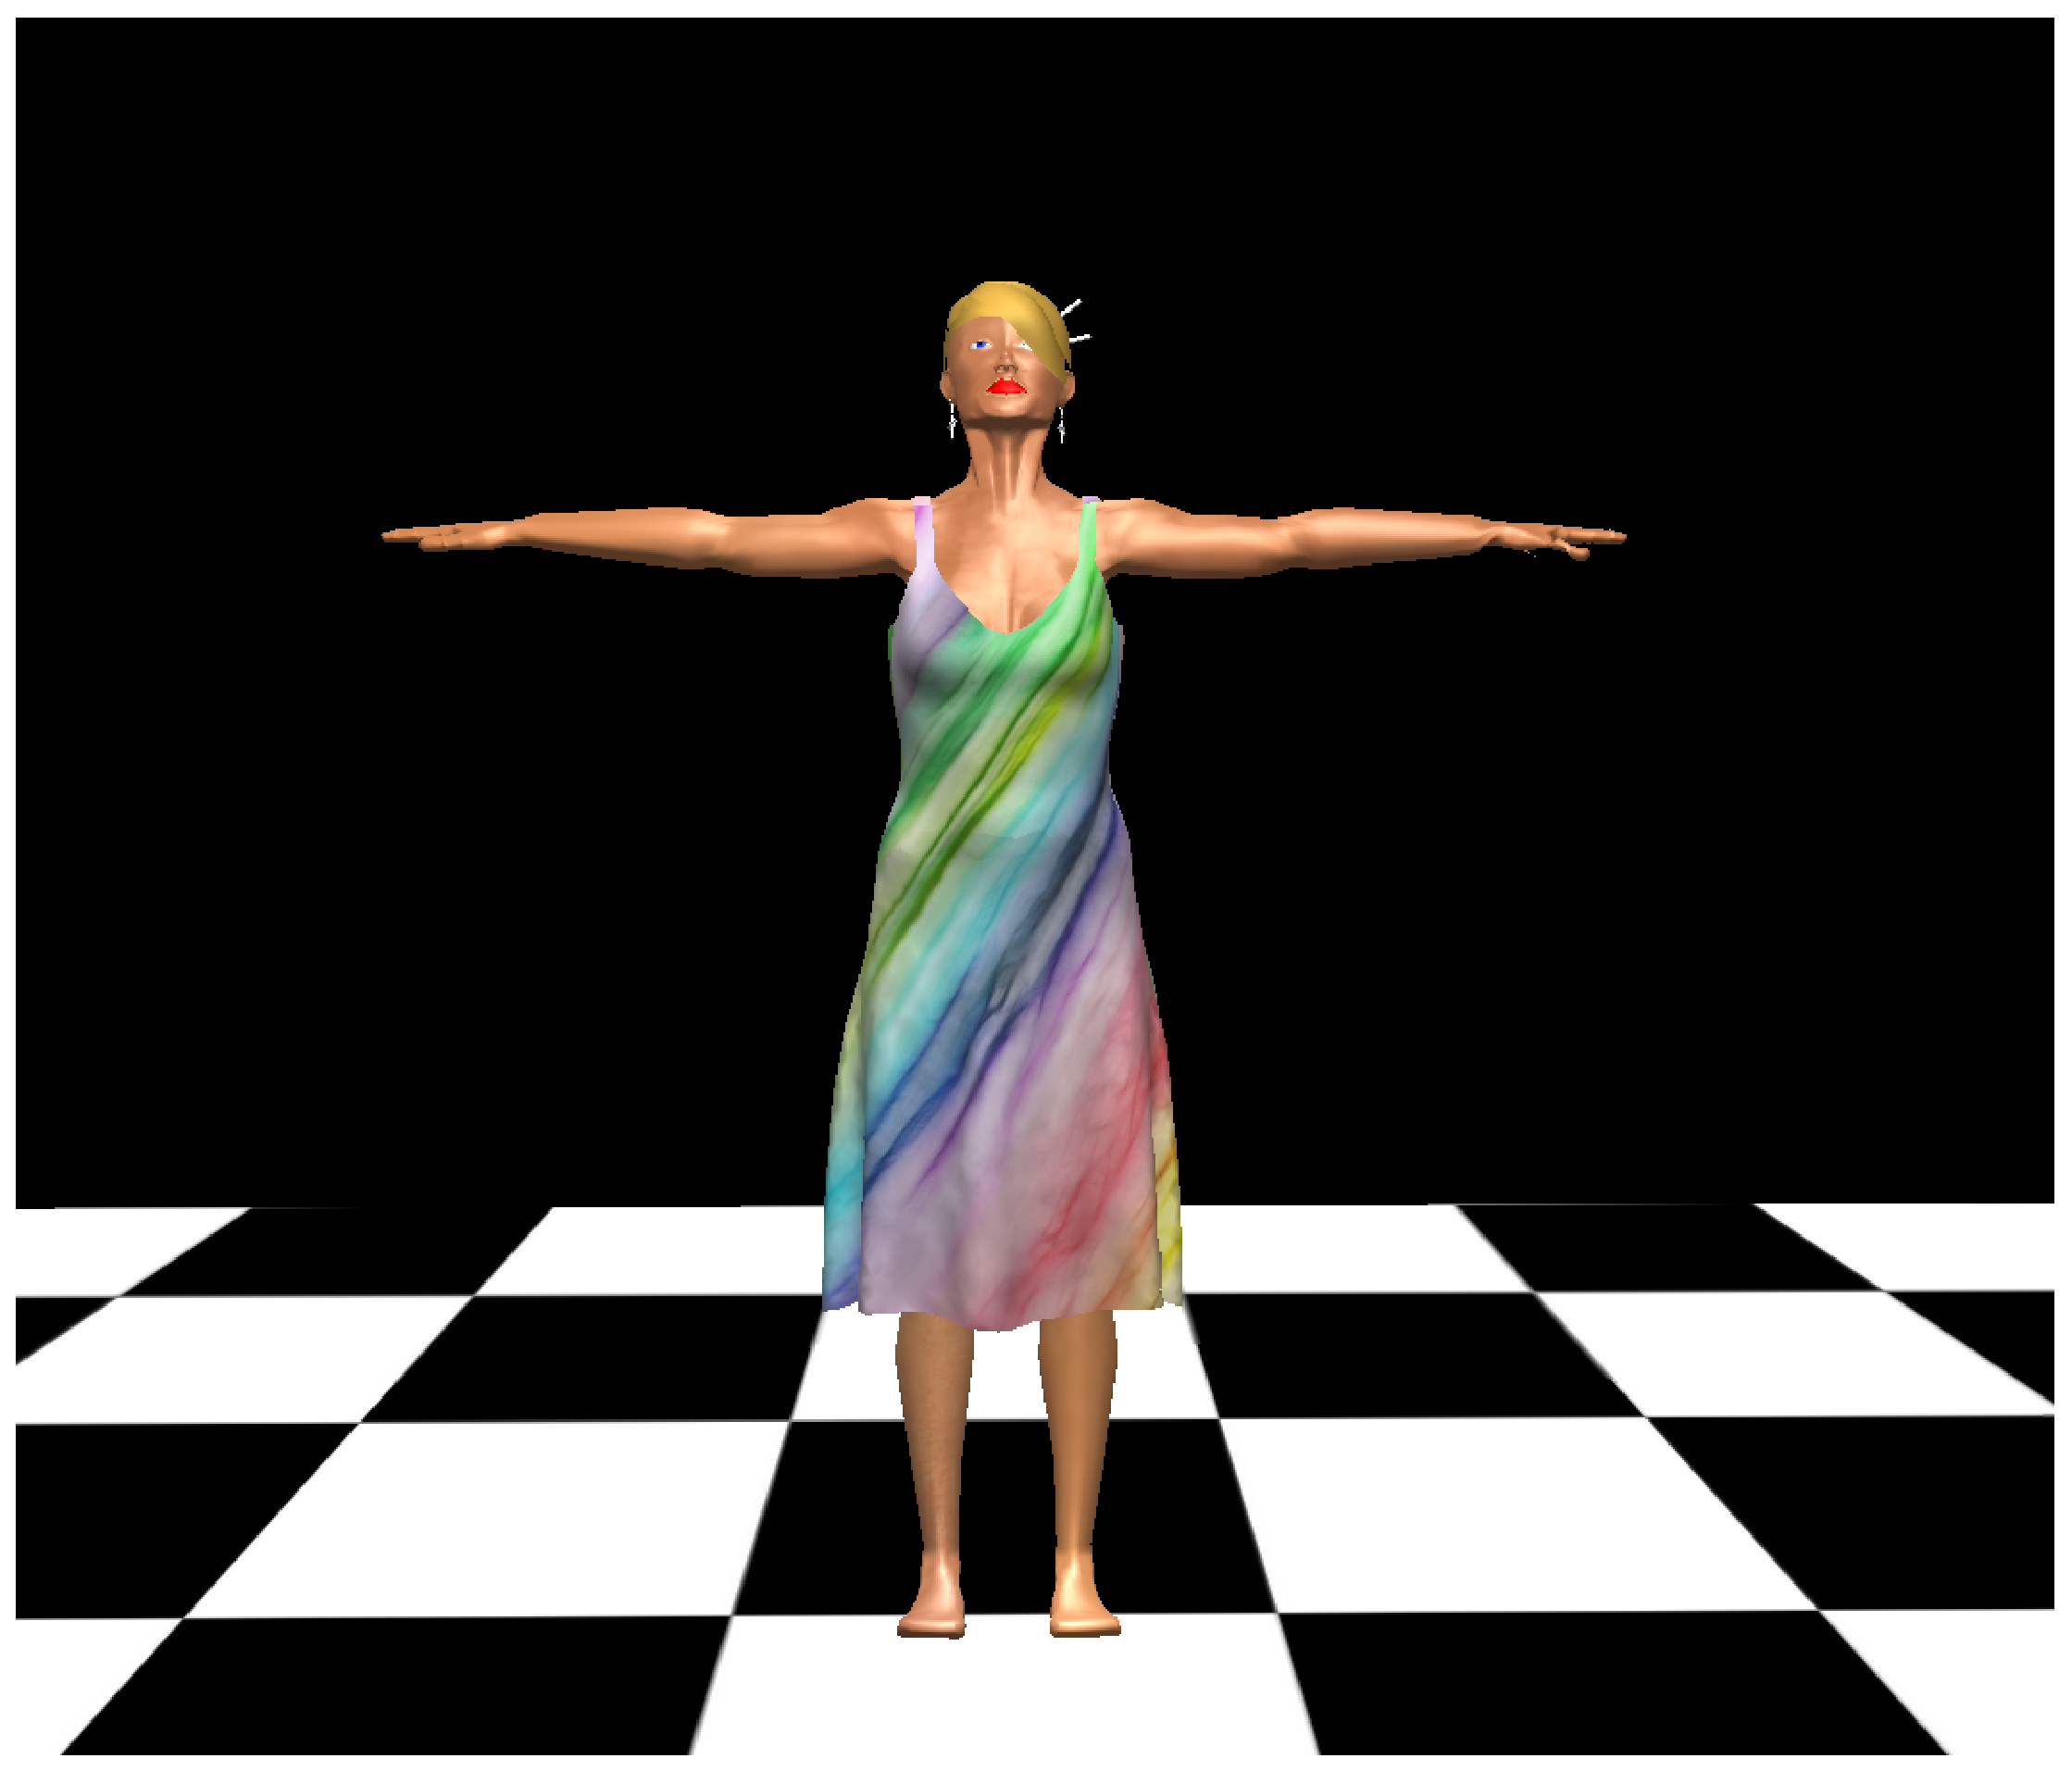
\includegraphics[width=0.333\textwidth]{./figures/sundress.eps}
	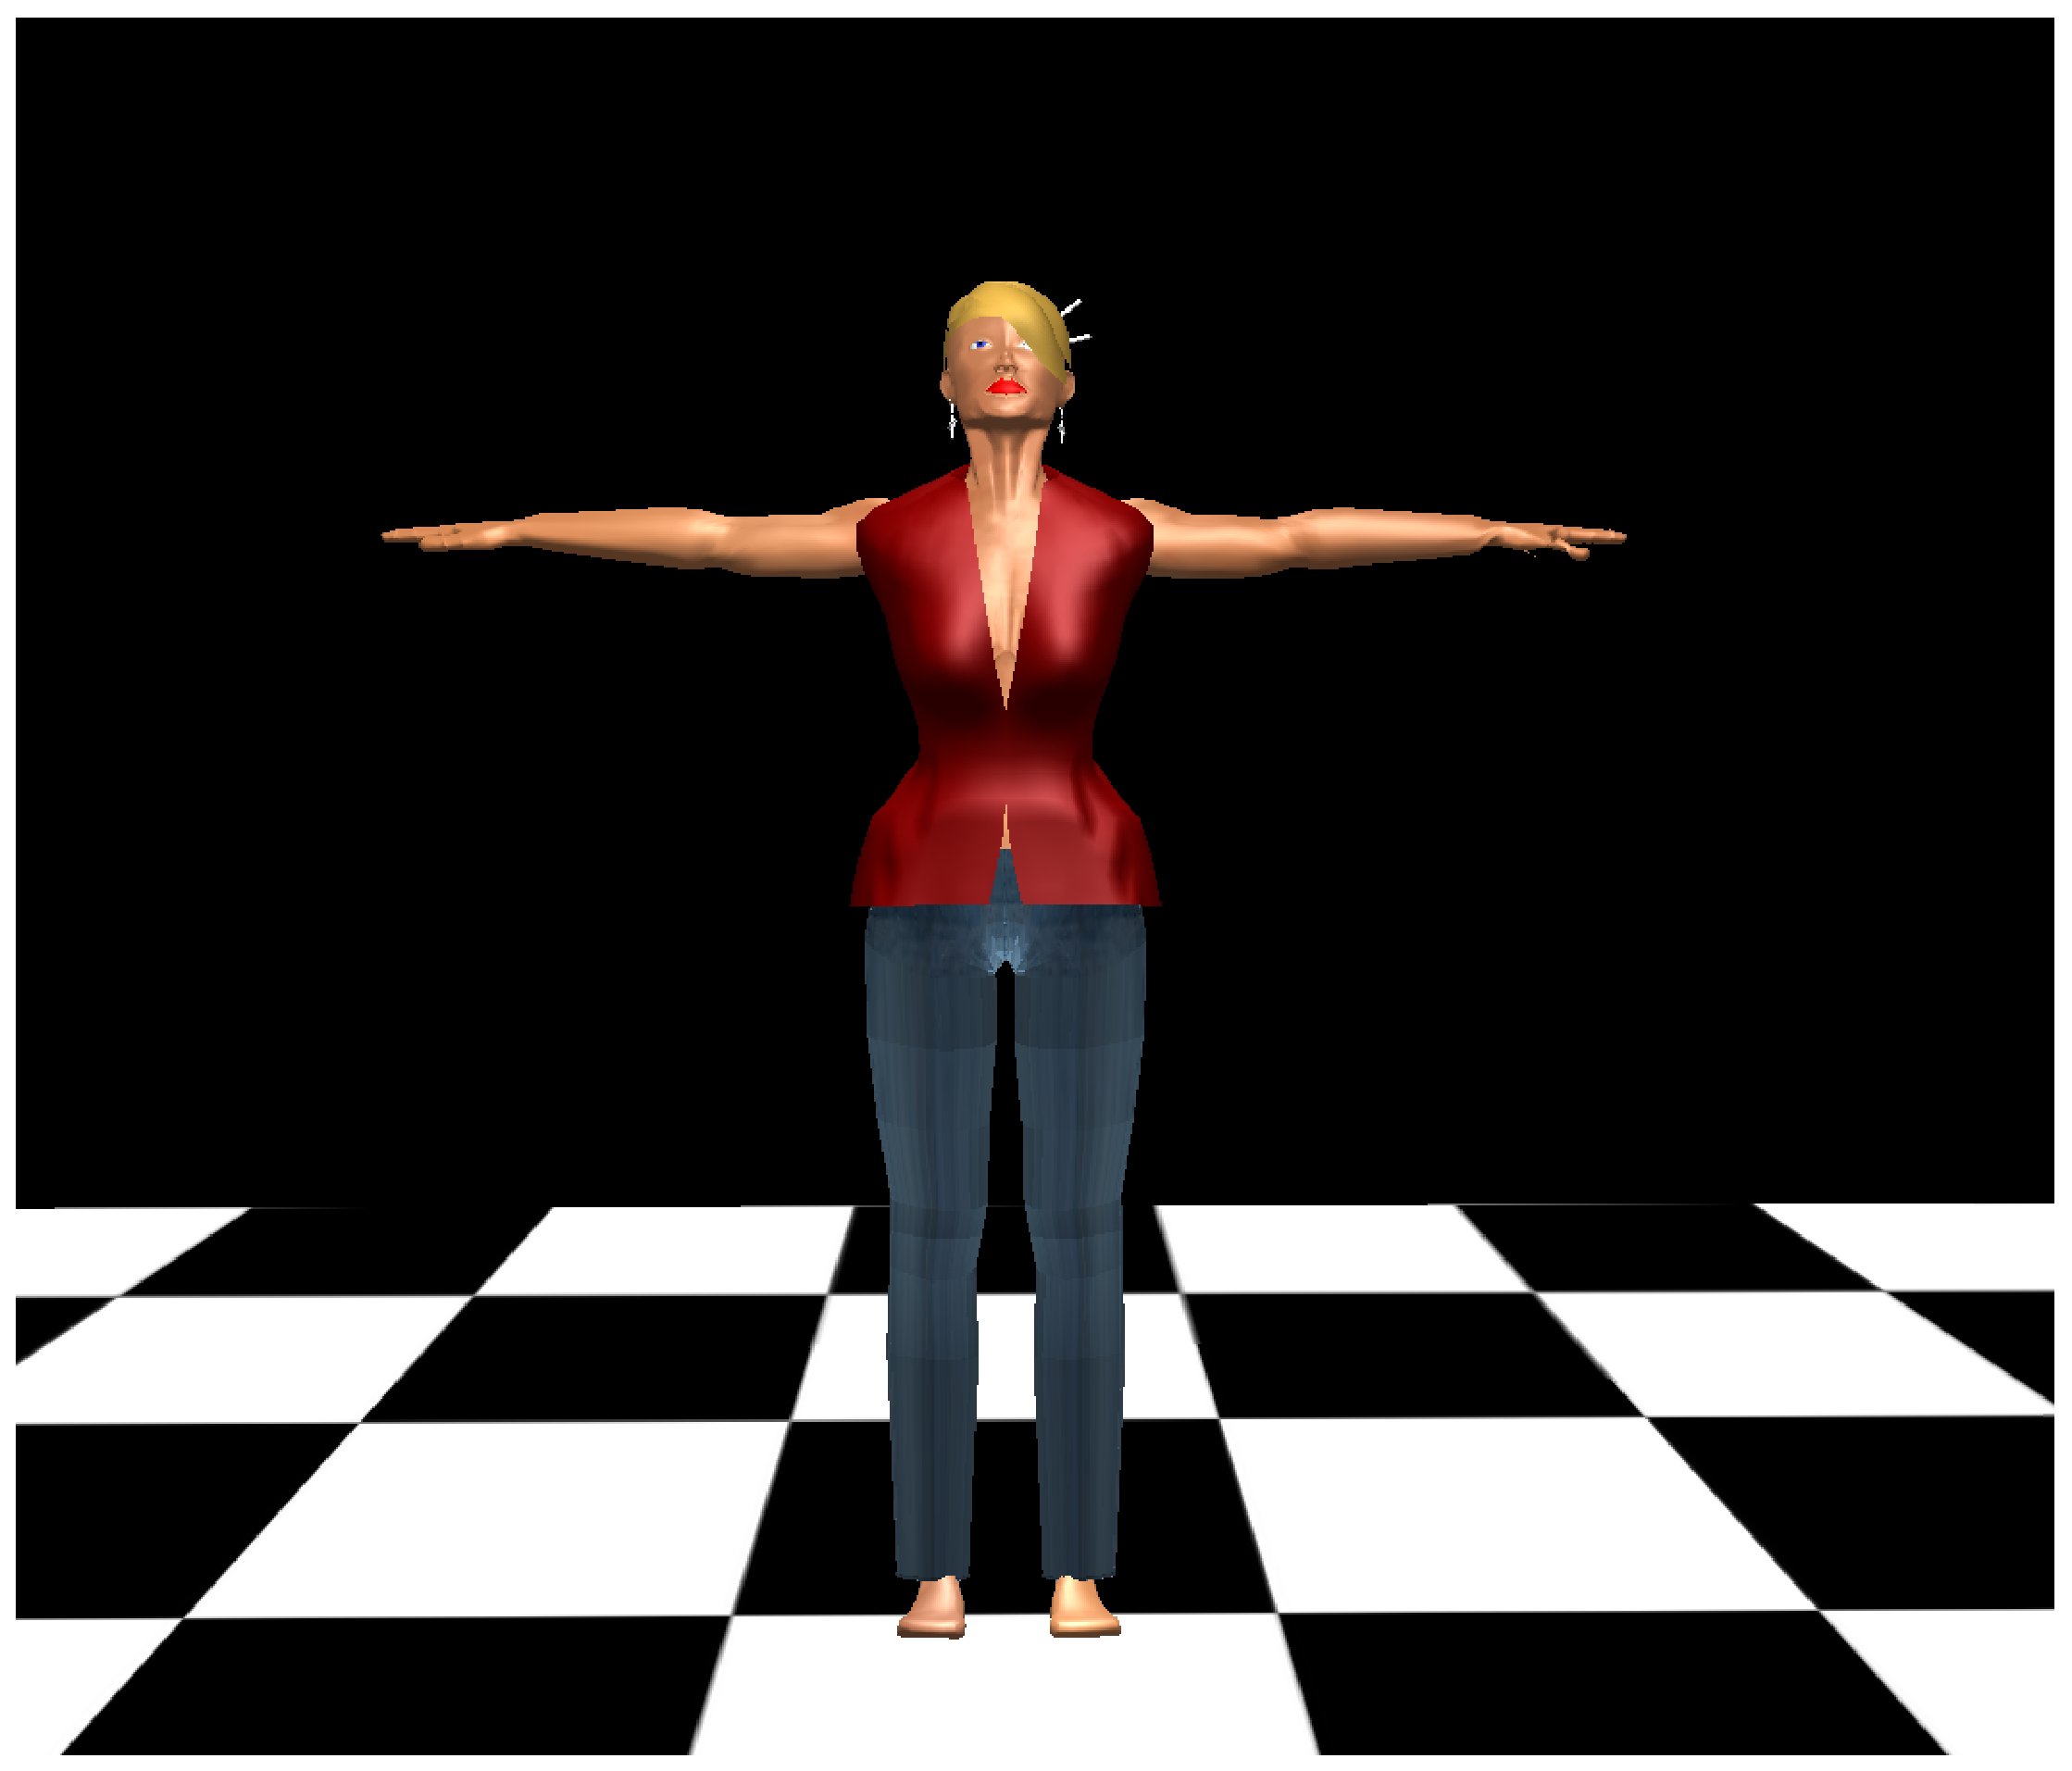
\includegraphics[width=0.333\textwidth]{./figures/jeans.eps}
	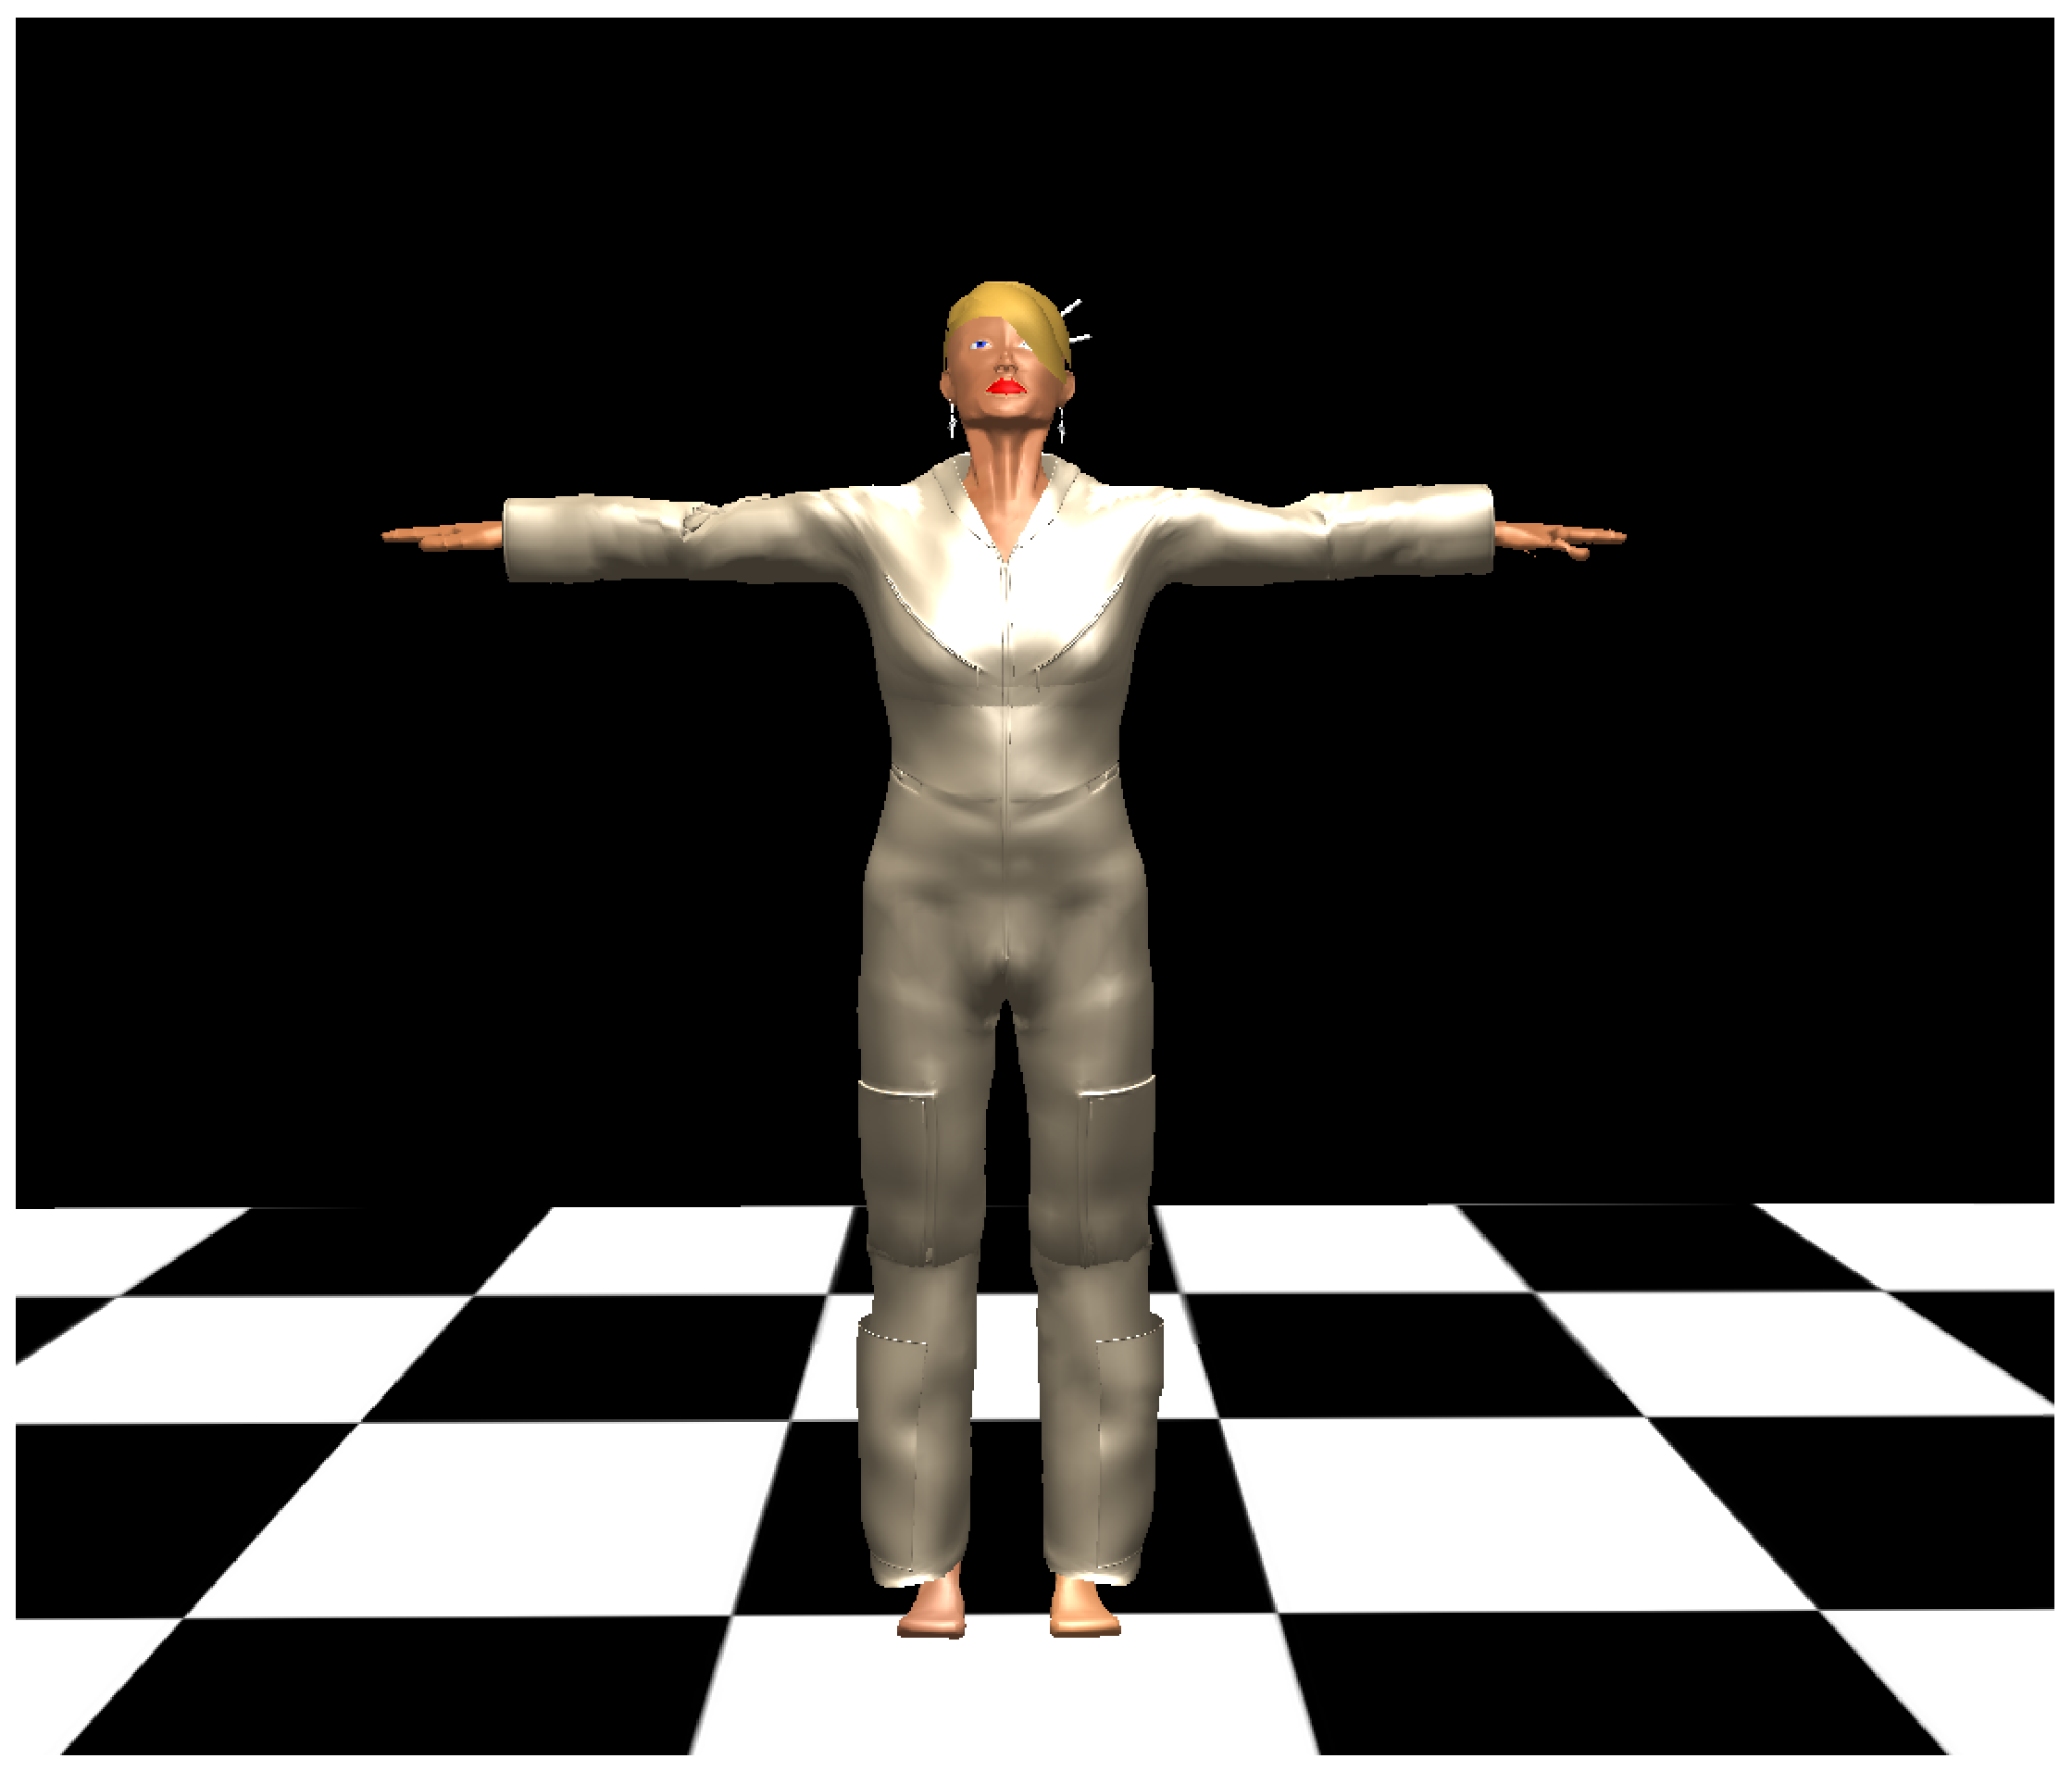
\includegraphics[width=0.333\textwidth]{./figures/flight.eps}
	}
	\centerline{(a)}
	\centerline{\ }
	\centerline{
	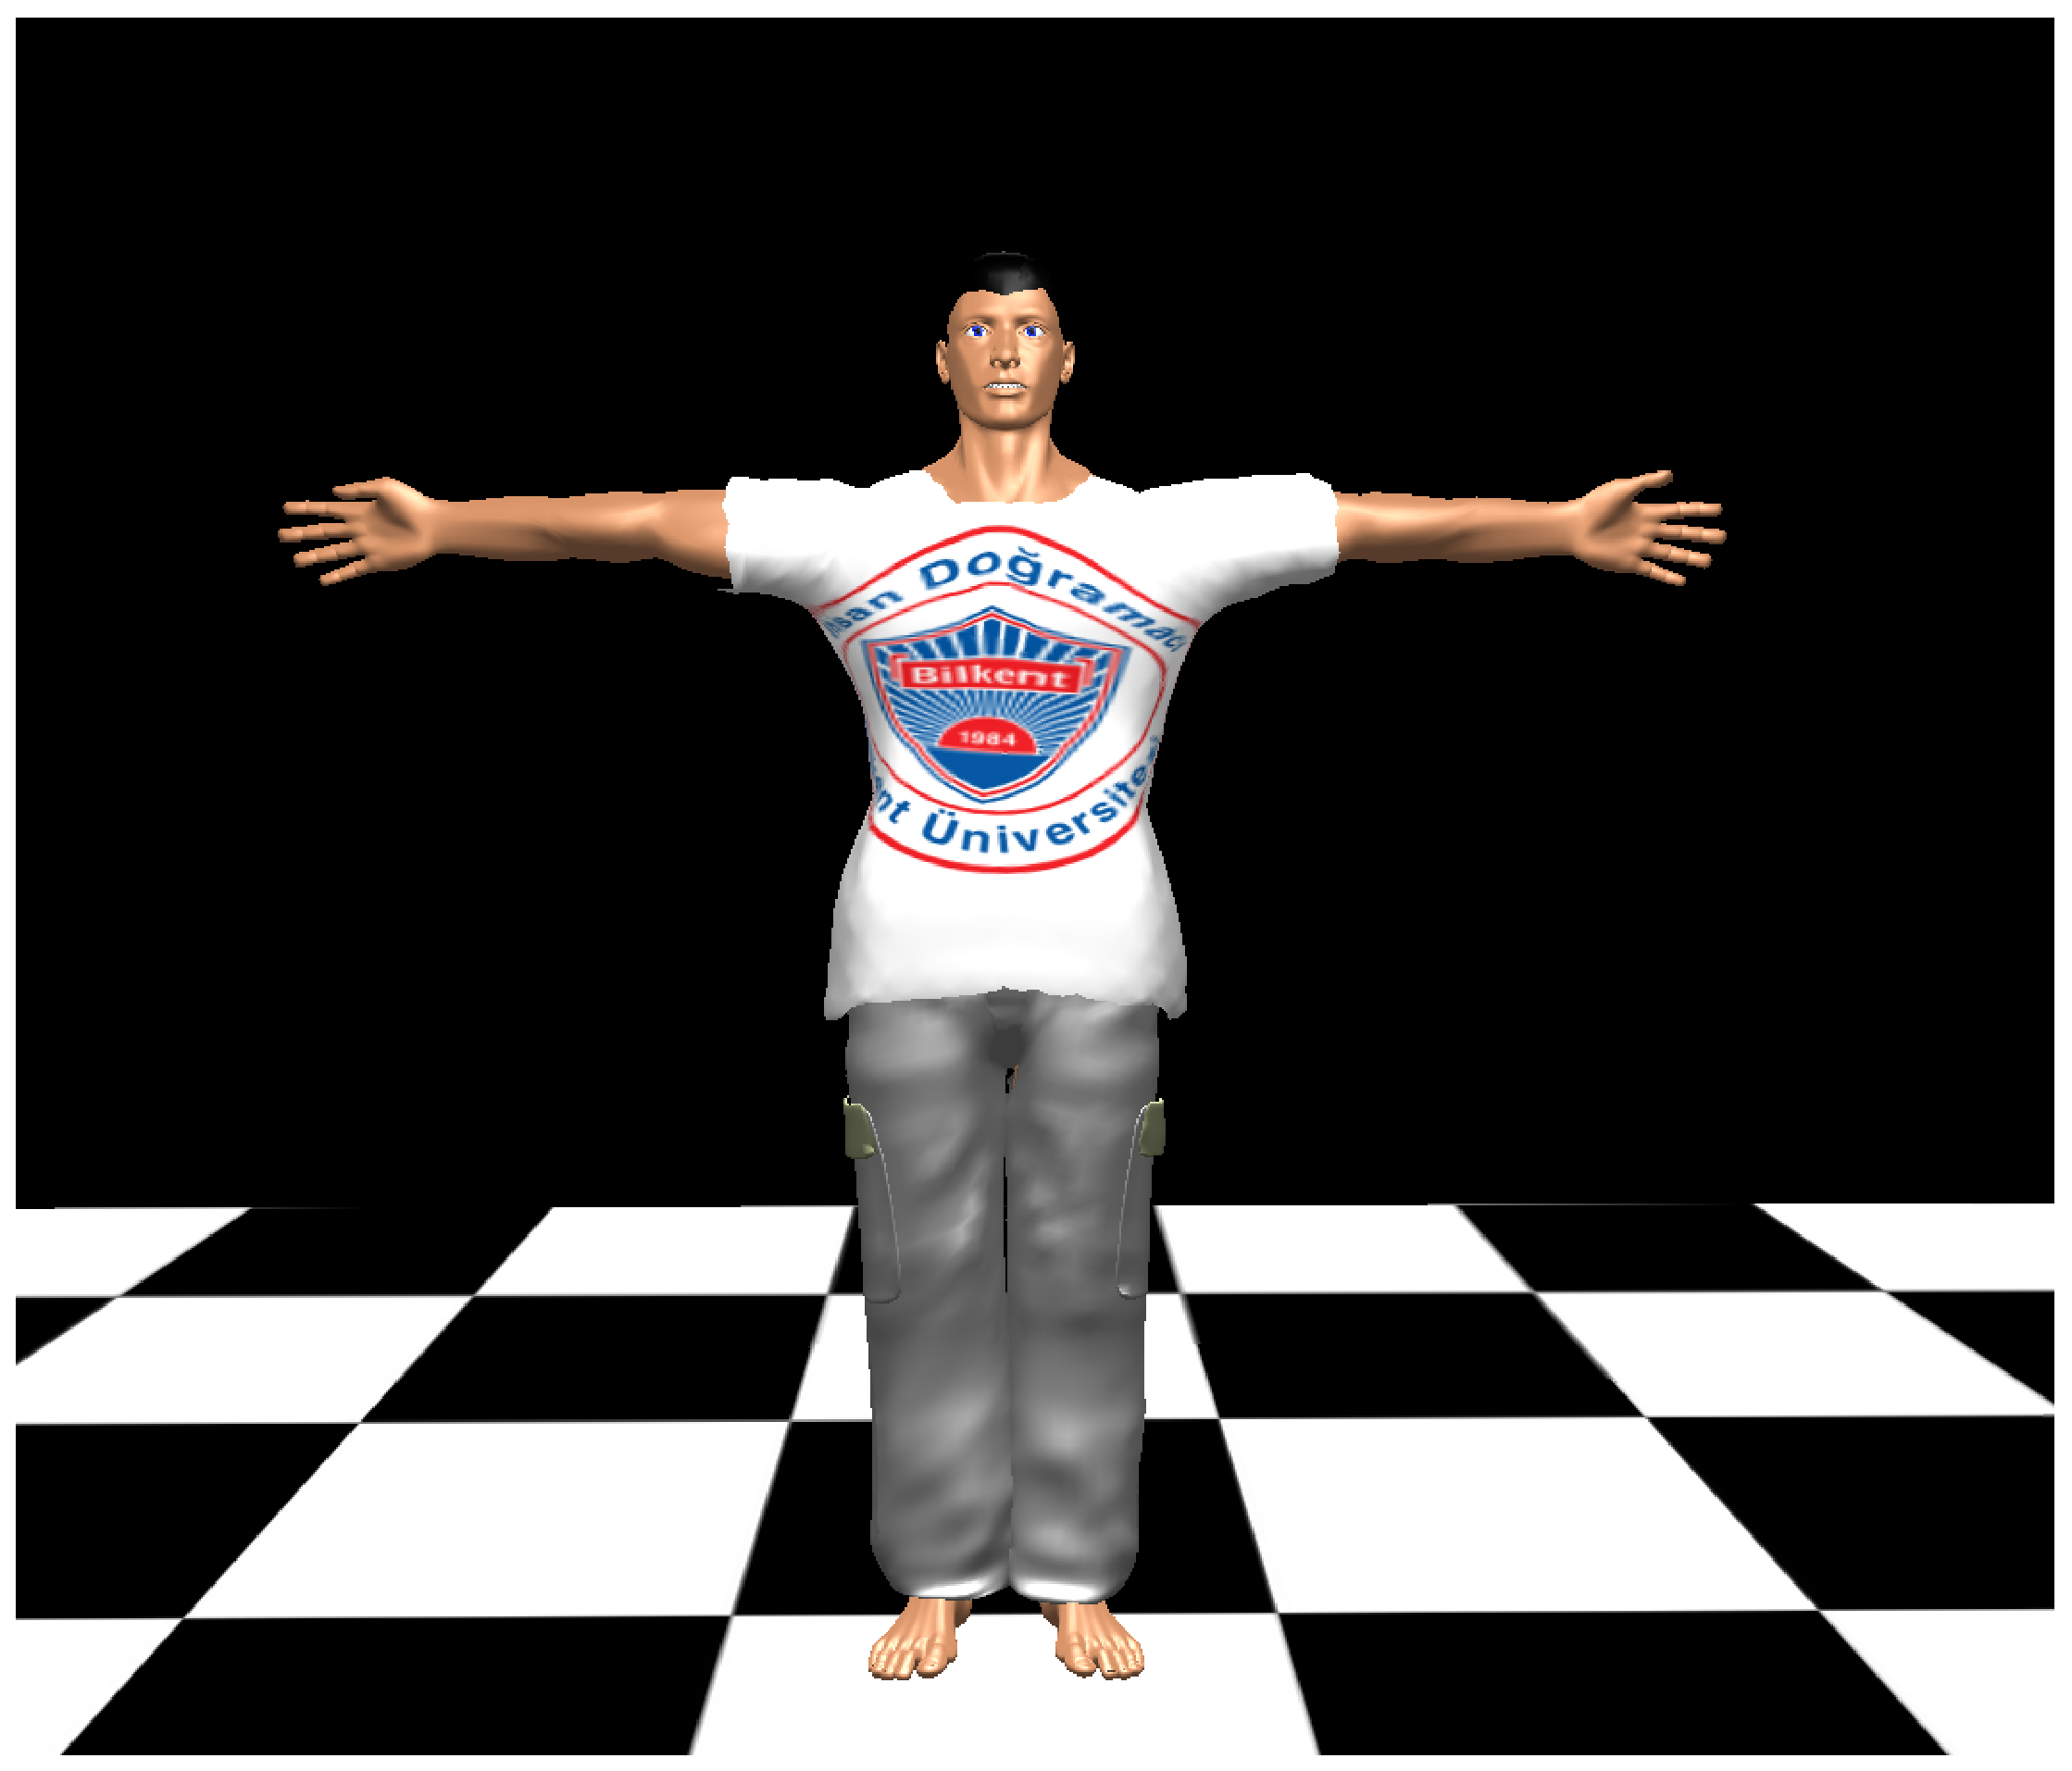
\includegraphics[width=0.333\textwidth]{./figures/shirt.eps}
	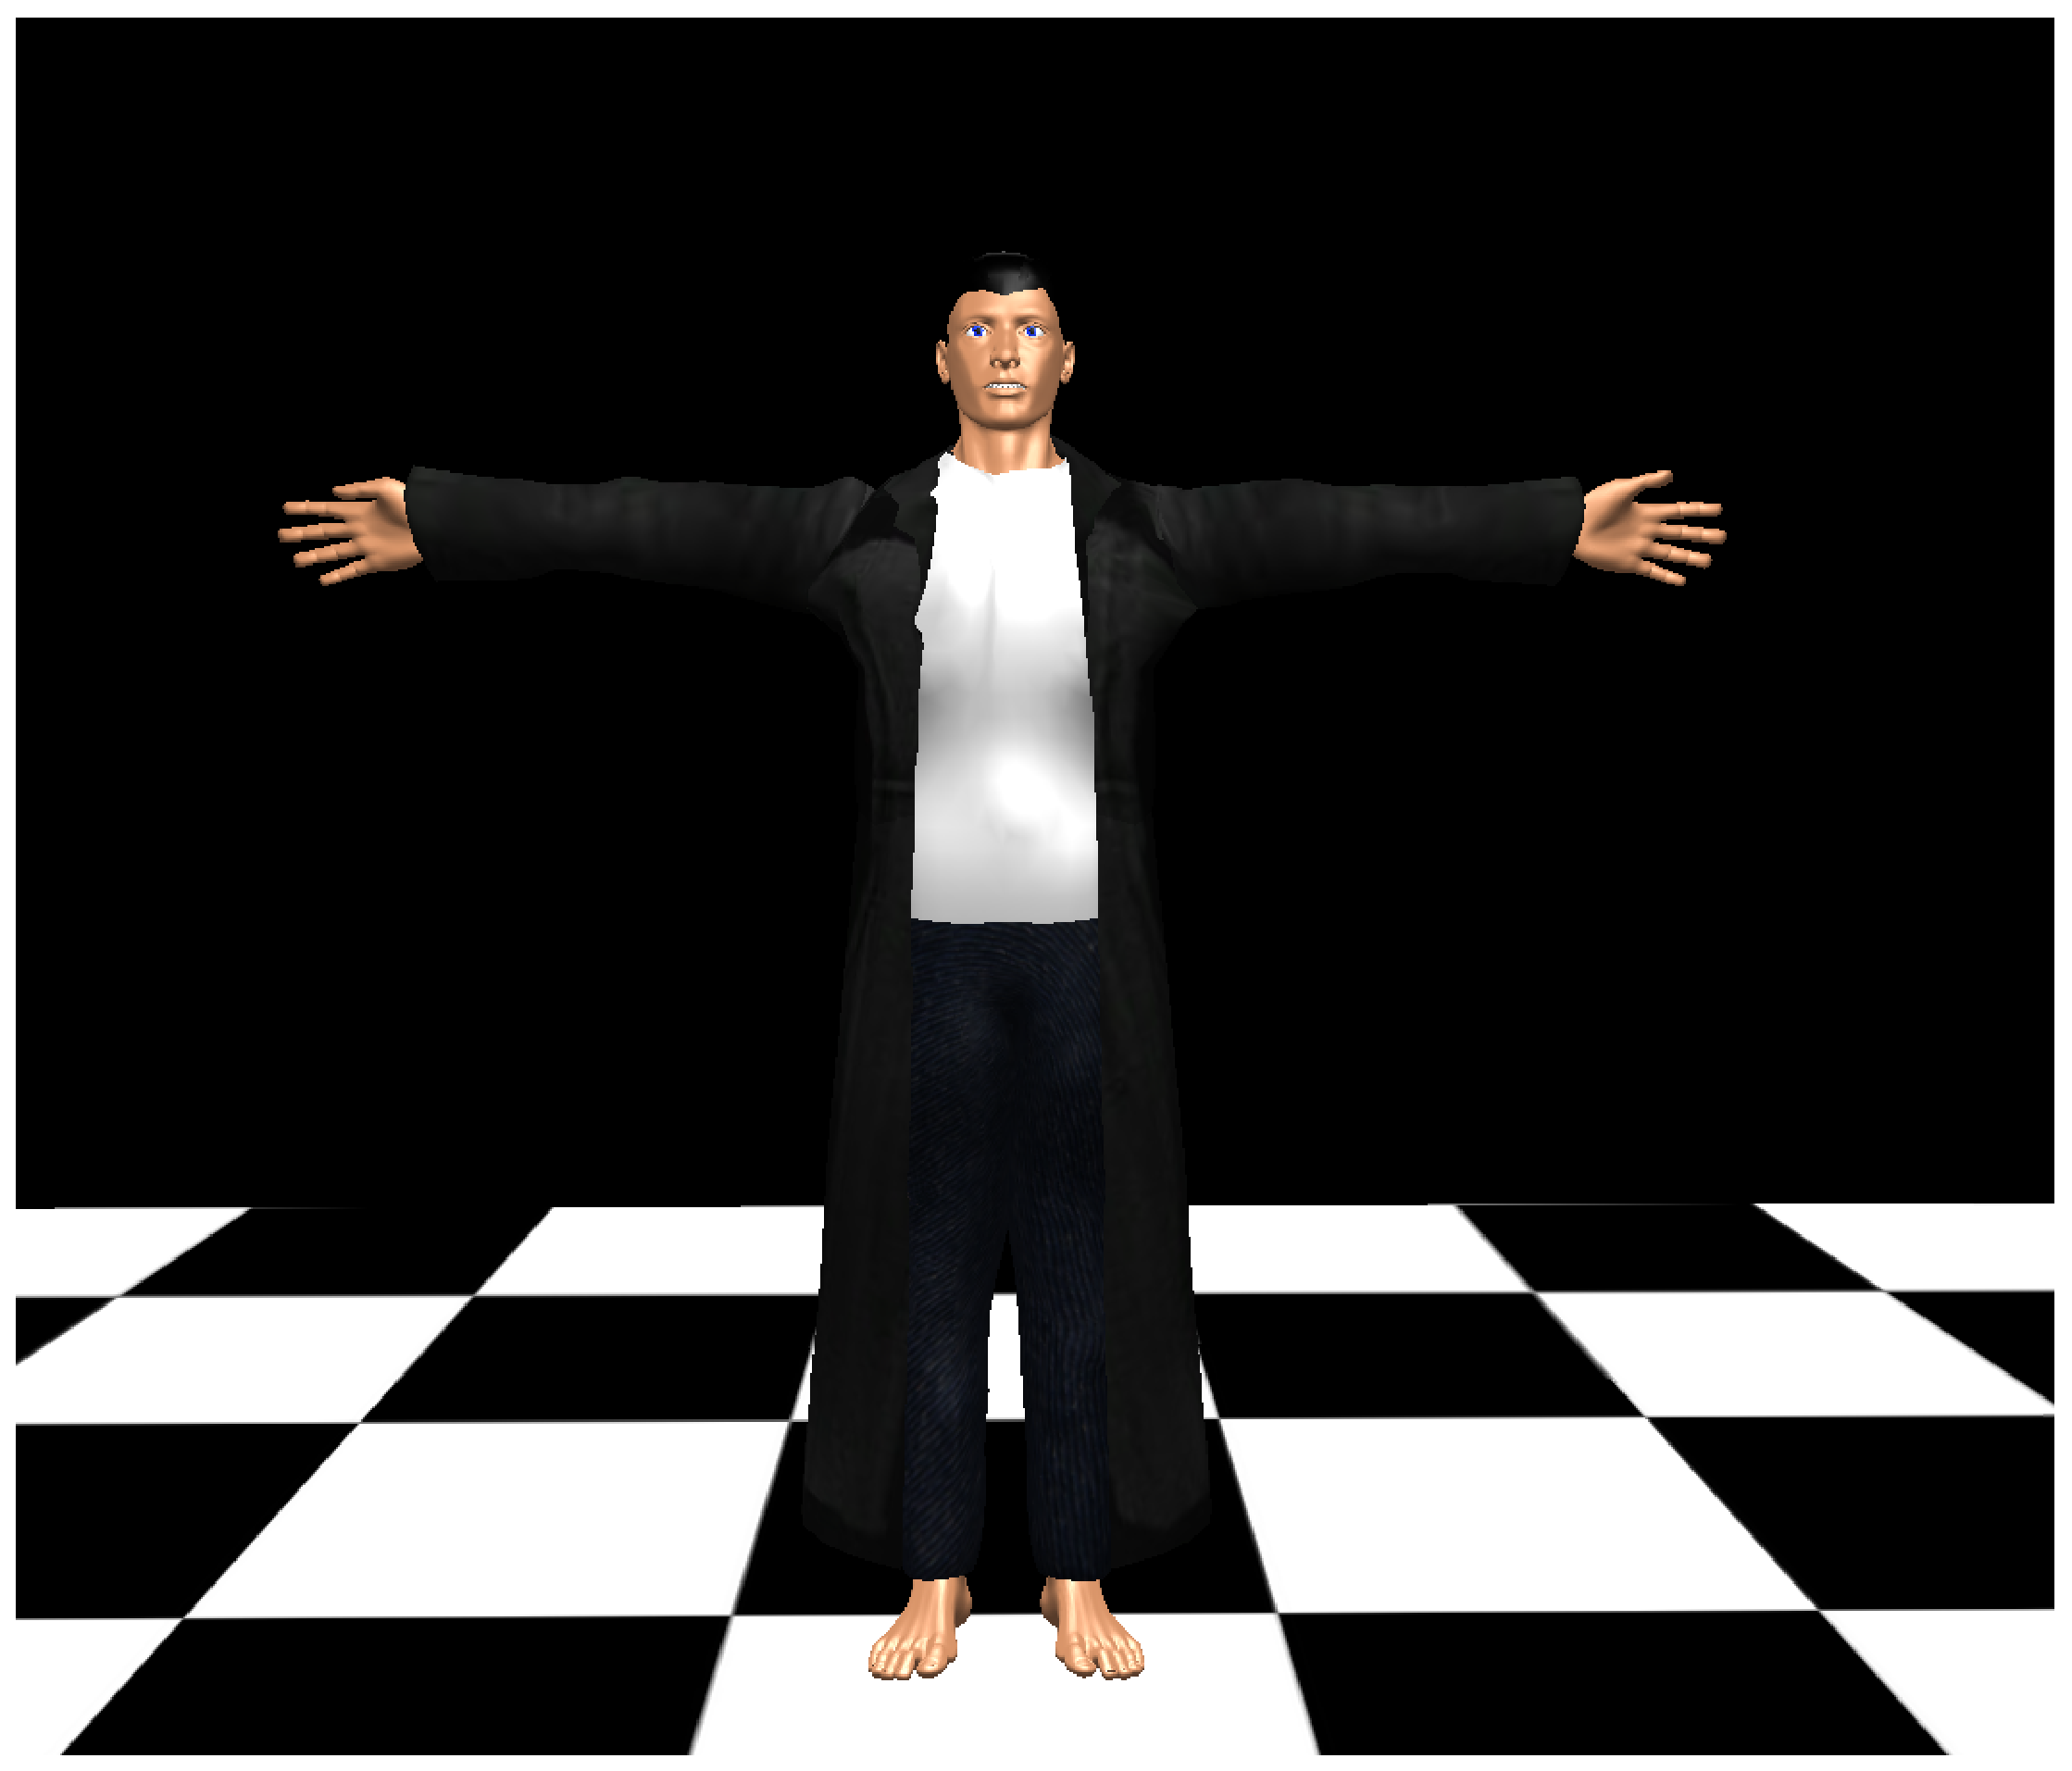
\includegraphics[width=0.333\textwidth]{./figures/duster.eps}
	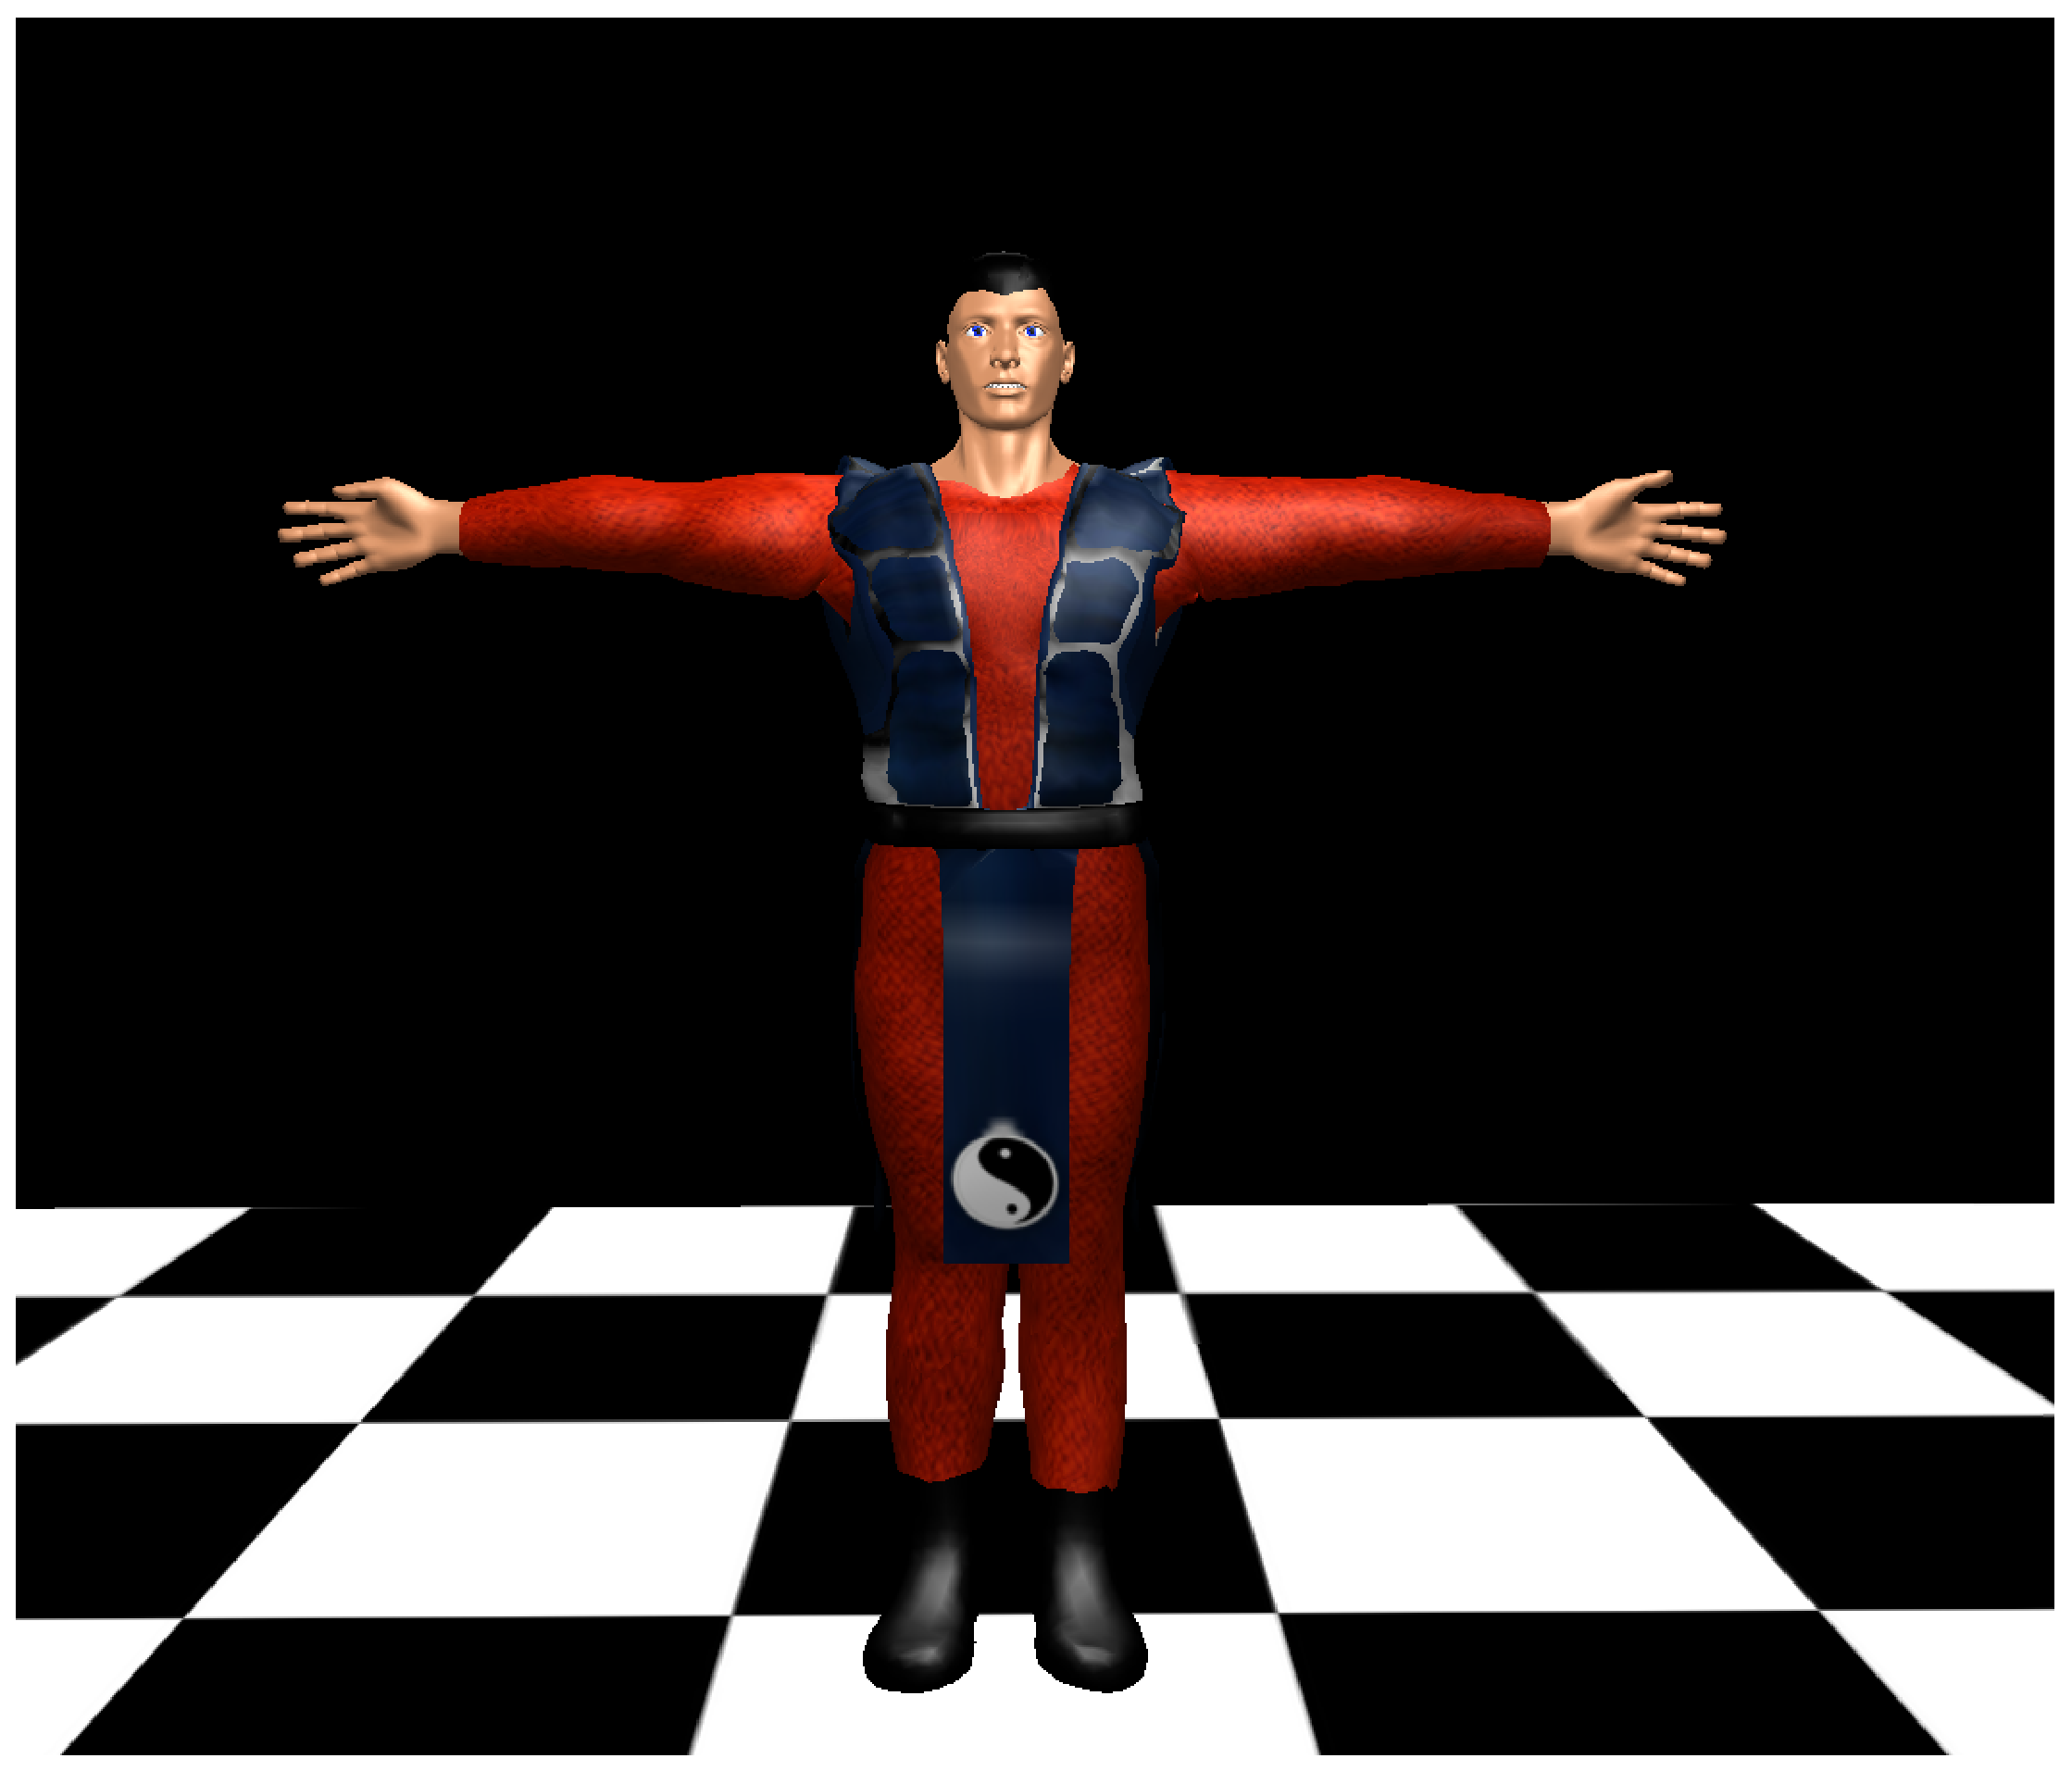
\includegraphics[width=0.333\textwidth]{./figures/martial.eps}
	}
	\centerline{(b)}
	\caption{The designed apparel meshes for the male and female avatars.}
	\label{fig:apparels}
\end{figure}


\clearpage

\section{Conclusion and Future Work}
\label{sec:Conclusions}

We propose a novel virtual fitting room using depth sensor data. The framework yields a realistic fitting experience with customized motion filters, body measurement and physical simulation. The proposed scaling method adjusts the avatar's body size parameters and determines a suitable apparel size, prepares the collision mesh and the physics simulation, within a total preprocessing time of one second. We apply real-time motion filters that prevent unnatural artifacts by smoothing the depth sensor data and estimate the locations of self-occluded body parts. Bone splitting is used to approximate the behavior of double bones in lower arms and legs for realistic animation and rendering of the body parts near the joints.

As a future work, we would like to improve the quality of the measurements by using data from an RGB sensor as well, because it provides additional valuable data. We would also like to increase the number of collision spheres for better collision detection.
 


\begin{thebibliography}{}
\bibitem{Fitnect2012}
Fitnect Interactive Kft. 3D Virtual Fitting Dressing Room / Mirror. Available at \verb+http://www.fitnect.hu/+. Accessed at June 2013.

\bibitem{Styku2013}
Styku, Inc. Virtual Fitting Room and Body Scanning. Available at \verb+http://www.styku.com/+. Accessed at June 2013.

\bibitem{FaceCake2013}
FaceCake Marketing Technologies, Inc. Visual Demonstration System. Available at \verb+http://www.facecake.com/+. Accessed at June 2013.

\bibitem{Protopsaltou2002}
D. Protopsaltou, C. Luible, M. Arevalo-Poizat, and N. Magnenat-Thalmann. A Body and Garment Creation Method for an Internet-based Virtual Fitting Room. \textit{Proceedings of Computer Graphics International (CGI '02)}, pages 105-122, Springer, Berlin, 2002.

\bibitem{Zhang2008}
W. Zhang, T. Matsumoto, J. Liu, M. Chu, and B. Begole. An Intelligent Fitting Room Using Multi-Camera Perception. \textit{Proceedings of the 13th International Conference on Intelligent User Interfaces (IUI '08)}, pages 60-69, ACM, New York, NY, USA, 2008.

\bibitem{Cheung2005}
K.-M. Cheung, S. Baker, and T. Kanade. Shape-From-Silhouette Across Time, Part II: Applications to Human Modeling and Markerless Motion Tracking. \textit{International Journal of Computer Vision}, 63(2):225-245, 2005.

\bibitem{Changa2011}
Y.-J. Changa, S.-F. Chenb, and J.-D. Huang. A Kinect-based System for Physical Rehabilitation: A Pilot Study for Young Adults with Motor Disabilities. \textit{Research in Developmental Disabilities}, 32(6):2566-2570, 2011.

\bibitem{Henry2012}
P. Henry, M. Krainin, E. Herbst, X.F. Ren, and D. Fox. RGB-D Mapping: Using Kinect-style Depth Cameras for Dense 3D Modeling of Indoor Environments. \textit{The International Journal of Robotics Research}, 31:647-663, 2012.

\bibitem{Gallo2012}
L. Gallo, A.P. Placitelli, and M. Ciampi. Controller-free Exploration of Medical Image Data: Experiencing the Kinect. 
\textit{Proceedings of the 24th International Symposium on Computer-Based Medical Systems (CBMS)}, pages 1-6, 2011.

\bibitem{Meng2010}
Y. Meng, P.Y. Mok, and X. Jin. Interactive Virtual Try-on Clothing Design Systems. \textit{Computer-Aided Design}, 42(4): 310-321, 2010.

\bibitem{Giovanni2012}
S. Giovanni, Y.C. Choi, J. Huang, K.E. Tat, and K. Yin. Virtual Try-On Using Kinect and HD Camera. \textit{Proceedings of the 
5th International Conference on Motion in Games (MIG'12), Lecture Notes in Computer Science}, vol. 7660, pages 55-65, Springer, Berlin, 2012.

\bibitem{OpenNI2013}
OpenNI Consortium. OpenNI - The Standard Framework for 3D Sensing. Available at \verb+http://www.openni.org/+. Accessed at June 2013.

\bibitem{Microsoft2013}
Microsoft, Inc. Kinect for Windows. Available at \verb+http://www.microsoft.com/en-us/kinectforwindows/+. Accessed at June 2013.

\bibitem{Hauswiesner2013}
S. Hauswiesner, M. Straka, and G. Reitmayr. Virtual Try-on Through Image-based Rendering. \textit{IEEE Transactions on Visualization
and Computer Graphics}, In press.

\bibitem{Zhou2012}
X. Zhou, B. Shu, S. Zhuo, X. Deng, P. Tan, and S. Lin. Image-based Clothes Animation for Virtual Fitting. \textit{SIGGRAPH Asia Technical Briefs}, Article 33, 4 pages, ACM, New York, NY, USA, 2012.

\bibitem{Khoshelham2012}
K. Khoshelham and S.O. Elberink. Accuracy and Resolution of Kinect Depth Data for Indoor Mapping Applications. \textit{Sensors}, 
12:1437-1454, 2012.

\bibitem{Matyunin2011}
S. Matyunin, D. Vatolin, Y. Berdnikov, and M. Smirnov. Temporal Filtering for Depth Maps Generated by Kinect Depth Camera. 
\textit{Proceedings of the 3DTV Conference: The True Vision - Capture, Transmission and Display of 3D Video (3DTV-CON)}, pages 1-4,
2011.

\bibitem{Cui2013}
Y. Cui Y., W. Chang, T. N\"{o}ll, and D. Stricker. KinectAvatar: Fully Automatic Body Capture Using a Single Kinect. 
\textit{Proceedings of the 11th Asian Conference on Computer Vision (ACCV 2012) Workshops, Lecture Notes in Computer Science}, 
vol. 7729, pages 133-147, Springer, Berlin, 2013.

\bibitem{Cui2010}
Y. Cui, S. Schuon, D. Chan, S. Thrun, and C. Theobalt. 3D Shape Scanning with a Time-of-flight Camera. \textit{Proceedings of IEEE Conference on Computer Vision and Pattern Recognition (CVPR)}, pages 1173-1180, 2010.

\bibitem {Yasseen2013}
Z. Yasseen, A. Nasri, W. Boukaram, P. Volino, and N. Magnenat-Thalmann. Sketch-based Garment Design with Quad Meshes. 
\textit{Computer-Aided Design}, 45(2):562-567, 2013.

\bibitem{Cordier2003}
F. Cordier, H. Seo, and N. Magnenat-Thalmann.
Made-to-measure Technologies for an Online Clothing Store. 
\textit{IEEE Computer Graphics and Applications}, 23(1):38-48, 2003. 

\bibitem{Meng2012}
Y. Meng, C.C.L. Wang, and X. Jin.
Flexible Shape Control for Automatic Resizing of Apparel Products.
\textit{Computer-Aided Design}, 44(1):68-76, 2012. 
    
\bibitem{Wang2003}
C.C.L. Wang, Y. Wang, and M.M.F. Yuen.
Feature Based 3D Garment Design Through 2D Sketches.
\textit{Computer-Aided Design}, 35(7):659-672, 2003. 

\bibitem{Kim2003}
S.M. Kim and T.J. Kang.
Garment Pattern Generation from Body Scan Data.
\textit{Computer-Aided Design}, 35(7):611-618, 2003. 

\bibitem{Kim2013}
D.-E. Kim  and K. LaBat. Consumer Experience in Using 3D Virtual Garment Simulation Technology. 
\textit{Journal of The Textile Institute}, In press.

\bibitem{Kim2011}
T.-Y. Kim. Character Clothing in PhysX 3. \textit{ACM SIGGRAPH Asia Nvidia Tech Talks}, Hong Kong, 2011.

\bibitem{Mullera2007}
M. M\"{u}ller, B. Heidelberger, M. Hennix, and J. Ratcliff. Position Based Dynamics. \textit{Journal of Visual Communication and Image Representation}, 18(2):109-118, 2007.

\bibitem{Tonge2010}
R. Tonge. Collision detection in PhysX, Recent Advances in Real-Time Collision and Proximity Computations for
Games and Simulations. \textit{ACM SIGGRAPH Course Notes}, 2010.

\bibitem{CodeProject2011}
S. Raiten. Kinect -- Getting Started -- Become The Incredible Hulk. Available at \verb+http://www.codeproject.com/Articles/213034/Kinect-+ \verb+Getting-Started-Become-The-Incredible-Hulk+, 2011. Accessed at June 2013.

\bibitem{Willis2012}
B. Willis. Body Proportions in Art. \textit{Wunderland Web Design}, 2013.

\bibitem{Azimi2012}
M. Azimi. Skeletal Joint Smoothing, White Paper, Microsoft Corp. Available at \verb+http://msdn.microsoft.com/en-us/library/jj131429.aspx+, Accessed at June 2013.

\bibitem{Holt1957}
C.C. Holt. Forecasting Trends and Seasonals by Exponentially Weighted Averages. {\textit Carnegie Institute of Technology, Pittsburgh ONR Memorandum}, No. 52, 1957.

\bibitem{Kalekar2004}
P.S. Kalekar. Time Series Forecasting Using Holt-Winters Exponential Smoothing. {\textit Kanwal Rekhi School of Information Technology}
, 2004.

\bibitem {HANIM}
H-Anim. Humanoid Animation Working Group. Available at \verb+http://www.h-anim.org+, Accessed at June 2013.

\bibitem{Kavan2009}
L. Kavan, S. Collins, and C. O'Sullivan. Automatic Linearization of Nonlinear Skinning. {\textit Proceedings of the Symposium on Interactive 3D Graphics and Games (I3D '09)}, pages 49-56, ACM, New York, NY, USA, 2009.

\bibitem{Kovar2002}
Kovar, Lucas, John Schreiner, and Michael Gleicher. "Footskate cleanup for motion capture editing." Proceedings of the 2002 ACM SIGGRAPH/Eurographics symposium on Computer animation. ACM, 2002.

\bibitem{Ikemoto2006}
Ikemoto, Leslie, Okan Arikan, and David Forsyth. "Knowing when to put your foot down." Proceedings of the 2006 symposium on Interactive 3D graphics and games. ACM, 2006.

\bibitem{Mankyu2013}
Sung, Mankyu. "Automatic Fixing of Foot Skating of Human Motions from Depth Sensor." Multimedia and Ubiquitous Engineering. Springer Netherlands, 2013. 405-412.

\bibitem{IKAN2013}
Human Modeling and Simulation Laboratory, University of Pennsylvania, "Inverse Kinematics using Analytical Methods-IKAN" 2013

\bibitem{Tolani2000}
Tolani, Deepak, Ambarish Goswami, and Norman I. Badler. "Real-time inverse kinematics techniques for anthropomorphic limbs." Graphical models 62.5 (2000): 353-388.

\bibitem{Samejima2012}
I. Samejima, K. Maki, S. Kagami, M. Kouchi, and H. Mizoguchi. A Body Dimensions Estimation Method of Subject from a Few Measurement Items Using KINECT. {\textit Proceedings of the IEEE International Conference on Systems, Man, and Cybernetics (SMC)}, 2012.

\end{thebibliography}

\end{document}



